\documentclass[12pt,a4paper,twoside, openright]{book} %oneside
%\documentclass[11pt]{ETHthesis}

% Ein paar brauchbare Pakete, nach Bedarf zu/abschalten mit %

% f�r Deutsch: erlaubt sind D, E, F, I
\usepackage{E}
%ETH-Layout, erst nach der Sprache festlegen
\usepackage{ETHthesis}
%\initETHthesis

% oneside - solo fronte, twoside - fronte retro
% openright - prima pagina dei capitoli su pagina destra, openany - indifferentemente
%
\usepackage{graphicx}                 %Pacchetto per inserire le figure nel Latex
\usepackage{latexsym}
%\usepackage{amsfonts}                 %Pacchetto per inserire i caratteri matematici
\usepackage{mathrsfs}
\usepackage{amsmath}                 
\usepackage{makeidx}                  %Pacchetto per generare l'indice analitico
%\usepackage[latin9]{inputenc}         %Pacchetto per poter inserire direttamente nel testo
                                      %lettere accentate. Se si scrive in inglese
                                      %si pu� commentare
\usepackage[T1]{fontenc}              %Pacchetto che gestisce l'encoding T1



\renewcommand{\rmdefault}{ppl}                                                                                 %             PER CAMBIARE I FONT..SE POI VUOI TI DO LA LISTA :)



\usepackage[english]{babel}   %Pacchetto per la sillabazione delle parole
                                      %in italiano e in inglese

\usepackage{verbatim}                 %Pacchetti per stampare il codice
\usepackage{listings}                 %Pacchetti per stampare il codice
\usepackage{fancyvrb}                 %Pacchetti per stampare il codice
\usepackage{rotating}
\usepackage{epigraph}
\usepackage{multirow}
\usepackage{acronym}
\usepackage{array}
\usepackage{tabularx}
\usepackage{textcomp}

\usepackage[linkcolor=black,colorlinks=true,citecolor=black,filecolor=black,backref=page]{hyperref}
\usepackage{siunitx}
\sisetup{
load-configurations  = {abbreviations,binary},
product-units        = power,
list-units           = single,
list-final-separator = {, and },
range-phrase         = { -- },
separate-uncertainty
}

\setlength{\topmargin}{-10mm}
\setlength{\headheight}{5.mm}
\setlength{\headsep}{+15.mm}
\setlength{\textheight}{220mm}
\setlength{\footskip}{+20.mm}
\setlength{\textwidth}{161mm} %!!!
\setlength{\oddsidemargin}{0mm}
\setlength{\evensidemargin}{0mm}
\setlength{\parindent}{0pt}
\usepackage{cancel}
\usepackage{booktabs}
\usepackage{caption}
\usepackage{subcaption}

% keeps the distance between paragraphs constant
\setlength{\parskip}{1ex plus 0.0ex minus 0.0ex}

%math-mode stuff
\renewcommand{\vec}{\overrightarrow}
\newcommand{\pt}{p_{T}}
\renewcommand{\deg}{^{\circ}}
\newcommand{\half}{\dfrac{1}{2}}
\newcommand{\sqhalf}{\dfrac{1}{\sqrt{2}}}
\renewcommand{\d}{\partial}
\newcommand{\calD}{\mathcal{D}}
\renewcommand{\dag}{^\dagger}

\newcommand{\0}{^{0}}
\newcommand{\+}{^{+}}
\renewcommand{\-}{^{-}}
\newcommand{\inv}{^{-1}}

\newcommand{\To}{\rightarrow}
\newcommand{\D}{\Delta}

\newcommand{\Z}{\mathrm{Z}}
\newcommand{\W}{\mathrm{W}}
\renewcommand{\H}{\mathrm{H}}
\newcommand{\pz}{p_\zeta}

\newcommand{\met}{\cancel{E}_T}
\newcommand{\vecmet}{\vec{\cancel{E}_T}}
\newcommand{\GeV}{\, \mathrm{GeV}}
\newcommand{\AND}{\, \& \,}
\newcommand{\thetahat}{\hat{\boldsymbol\theta}}
\newcommand{\boldtheta}{\boldsymbol\theta}
\newcommand{\muhat}{\hat{\mu}}

%Frequently used particles
\newcommand{\eplus}{$e^{+}$}
\newcommand{\eminus}{$e^{-}$}
\renewcommand{\b}{$b$}
\renewcommand{\t}{$\tau$}
\newcommand{\piz}{$\pi^0$ \space}
\newcommand{\tauh}{$\tau_h$}


%variables and observables
\newcommand{\dEdx}{$dE/dx$}
\newcommand{\sqrts}{$\sqrt{s}$}
\renewcommand{\L}{$\mathcal{L}$}
\renewcommand{\l}{\mathcal{L}}
\newcommand{\LT}{$L_T$}
\newcommand{\Inv}{$^{-1}$}
\newcommand{\sq}{$^{2}$}
\renewcommand{\u}{$\mu$}
\newcommand{\DR}{$\Delta R$\ }
\newcommand{\pT}{$p_T$~}
\newcommand{\MET}{$\cancel{E}_T$\ }
\newcommand{\db}{$\D\beta$\ }
\newcommand{\Eta}{$\eta$~}
\newcommand{\abseta}{$|\eta|$~}

%other stuff
\renewcommand{\~}{$\sim$}
\newcommand{\um}{$\mu$m\ }
\newcommand{\chisq}{$\chi^2$}
\newcommand{\madgraph}{\textsc{MadGraph}}
\newcommand{\pythia}{\textsc{Pythia}}
\newcommand{\CLs}{CL$_s$}



%\newcommand{\uds}{$\Upsilon(2S)$}

\newcommand{\anti}[1]{\overline{#1}}
\newcommand{\fixed}{\frac{\ulcorner \urcorner}{\llcorner \lrcorner}}
\newcommand{\bold}[1]{\textbf{#1}}
\newcommand{\blankpage}{\clearpage\mbox{}\clearpage}
\renewcommand{\rm}[1]{\mathrm{#1}}
\newcommand{\opname}[1]{\operatorname{#1}}
\renewcommand{\slash}[1]{\cancel{#1}}
\renewcommand{\bar}[1]{\overline{#1}}
\newcommand{\ket}[1]{|#1\big{>}}
\newcommand{\spinor}[2]{\left(\begin{array}{c}#1 \\#2\end{array}\right)}
\newcommand{\spinmatrix}[4]{\left(\begin{array}{cc}#1 & #2 \\#3 & #4\end{array}\right)}
\input{src/environments.tex}


\begin{document}

% frontmatter
\frontmatter
    \begin{titlepage}
      \setlength{\baselineskip}{8mm}
      \vspace{1cm}
     \begin{center}
       {\def\\{\linebreak}
        \huge\bf This is not the greatest title in the world, this is just a tribute}
      \end{center}
      \vspace{1cm}
      \begin{center}
        \Large Dissertation  \\%\linebreak
        \vspace{0.4cm}
        \large zur  \\
        \vspace{0.4cm}
        \Large Erlangung der naturwissenschaftlichen Doktorw\"urde \\ %\linebreak
        \Large (Dr. sc. nat.) \\
        \vspace{0.4cm}
        \large vorgelegt der \\
        \vspace{0.4cm} 
        \Large Mathematisch-naturwissenschaftlichen Fakult\"at \\
        \vspace{0.4cm}
        \large der \\
        \vspace{0.4cm}
        \Large Universit\"at Z\"urich \\
      \end{center}
      \vspace{0.2cm}
    \begin{center}
      \large von \\
      \LARGE Mauro Verzetti \\
       \vspace{0.2cm}
       %\acatitlestring \\%\linebreak
        \large aus \\
        \vspace{0.2cm}
        \Large Italien \\
      \end{center}
      \begin{center}
        \large Promotionkomitee \\%\linebreak
        \vspace{0.2cm}
        \Large Prof. Dr. V. Chiochia \\%\linebreak
       \vfill
       \large Z\"urich, 2014       
      \end{center}
      \vspace{1.0cm}
\cleardoublepage
    \end{titlepage}

\blankpage 
\chapter*{Abstract}

Diese Dissertation stellt die Ergebnisse der Suche nach dem Standardmodell-Prozess $pp \To \W\H \To \ell \nu \tau_\ell \tau_h$, in dem das Higgs-Boson in Tau-Leptonen zerf\"allt, wobei eines der Tau-Leptonen hadronisch zerf\"allt, dar. Die Anwesenheit eines zus\"atzlichen Leptons aus dem W-Boson-Zerfall f\"uhrt zu einer starken Reduzierung des Untergrunds in diesem Kanal.

Das Higgs-Boson, welches urspr\"unglich von P. Higgs, F. Englert et al. 1964 vorhergesagt wurde, war lange Zeit das einzig fehlende, vom Standardmodell (SM) vorhergesagte Teilchen und war daher Kern vieler gro\ss{}er Anstrengungen in der experimentellen Teilchenphysik. Suchen nach diesem schwer zu entdeckendem Teilchen am LEP und auch am Tevatron waren erfolglos. Der Large Hadron Collider (LHC) und die beiden Hauptexperimente (ATLAS und CMS) wurden haupts\"achlich gebaut, um Fortschritte in der Suche nach dem Higgs-Boson zu erzielen.

Die Anstrengungen machten sich am 4. Juli 2012 bezahlt, als beide Experimente die Entdeckung einer Resonanz um 125 GeV in den Spektren der $\gamma \gamma$ und der ZZ Endzust\"ande bekannt gaben. Obwohl diese Nachricht enthusiastisch aufgenommen wurde, mussten fermionische Zerf\"alle dieser Resonanz erst noch entdeckt werden. Die Suche nach dem Zerfallsprozess $\rm{H} \To \tau \tau$ war der vielversprechendste Kanal um diesen Zerfall zu entdecken und stand im direkten Wettbewerb mit dem Zerfall $\rm{H} \To b\bar{b}$, der zwar ein gr\"o\ss{}eres Verzweigungsverh\"altnis besitzt, aber daf\"ur auch mit gr\"o\ss{}erem Untergrund zu k\"ampfen hat.

In dieser Arbeit konzentrieren wir uns auf die assoziierte Produktion eines Higgs-Bosons und eines W-Bosons, um m\"oglichst kleine Untergrundprozesse zu haben. Dieser Endzustand ist Teil eines gr\"o\ss{}eren Suchprogramms des CMS-Experiments, welches im ersten Kapitel dieser Arbeit kurz beschrieben wird.

Der Hauptuntergrund in diesem Endzustand setzt sich aus einer Reihe von Prozessen (haupts\"achlich Top-Quark- und W-Boson-Produktion zusammen mit Jets) zusammen, in denen mindestens eines der Leptonen im Endzustand aus der Fehlidentifizierung eines Quark- oder Gluonjets stammt. Um diese Untergrundquelle zu modellieren wird eine datengetriebene Methode entwickelt, die sogenannte k--Nearest Neighbors Classifier verwendet.

In dieser Suche wurde der Produktionswirkungsquerschnitt des Higgs-Bosons mit einer kombinierten Signalst\"arke von $\mu = -2.6\pm1.7$ gemessen, die unterhalb der SM-Erwartung liegt, jedoch mit dieser innerhalb eines Signifikanzniveaus von $2.1\,\sigma$ kompatibel ist.
Das Ergebnis dieser Analyse wurde mit anderen Suchen nach Tau-Lepton-Zerf\"allen des Higgs-Bosons im CMS-Experiment kombiniert und resultierte damit in der ersten Beobachtung dieses Prozesses.
%Die Suche schlie\ss{}t die Existenz eines SM-Higgs-Bosons mit einem Produktionswirkungsquerschnitt gr\o\ss{}er als 2,5-mal der SM-Erwartung aus. Die beobachtete Ausschlussgrenze ist innerhalb von $2\sigma$ konsistent mit der reinen Untergrundhypothese. Dieses Ergebnis wurde mit den anderen Suchen nach dem Higgs-Boson im Zerfall in Tau-Paare am CMS-Experiment kombiniert, welches letztendlich zur Beobachtung dieses Prozesses f\"uhrte.
\cleardoublepage 
\chapter*{Abstract}

This thesis presents the results of the search for the Standard Model process $\W\H \To \ell \tau_\ell \tau_h$, where the Higgs boson decays to tau leptons and one of them decays hadronically. The presence of the additional lepton form the decay of the W boson largely reduces the backgrounds in this channel.

The Higgs boson has been for long time the only missing particle predicted by Standard Model and has been therefore the target of major efforts in the experimental particle physics filed. Searches for this elusive particles have been conducted without any success both at LEP and Tevatron as a side project in their respective physics programme. The LHC and two of its major experiments (ATLAS and CMS) have been built with the main purpose of casting some light in this longstanding mystery. 

These efforts culminated on the 4$^{th}$ of july 2012, when both the experiments announced the observation of a resonance at 125 GeV in the $\gamma \gamma$ and ZZ spectra combined. While this announcement triggered a well deserved enthusiasm, the sign of the fermionic decays of this resonance were still to be observed. The search for the decay process $\rm{H} \To \tau \tau$ has been the most promising channel to first observe the decay of the SM Higgs boson to fermions. 

In this work we focus on the associated production of a Higgs boson and a W boson as a low--background environment to observe such decay. This final state is part of a wider $\rm{H} \To \tau \tau$ search program performed by CMS which is briefly outlined in the first chapter of this work. 

The main source of background in this peculiar final state comes from a wide range of processes (mainly $t\bar{t}$ and W plus jets) in which at least one of the leptons in the final state comes from a mis--identified quark or gluon jet. To model this source of backgrounds a fully data--driven method that exploits a k--Nearest Neighbors classifier is developed.

The final results do not show any presence of the Higgs boson, but rather an under--fluctuation of the backgrounds. Given the results an upper limit on the presence of the Higgs boson is set as a function of the Higgs mass.
\cleardoublepage 
\chapter*{Acknowledgements}

I first of all want to thank my advisor Prof Vincenzo Chiochia, for his trust in my abilities and his mentoring, which is of prime importance in such a large collaboration.

I owe special gratitude towards to Dr. Evan Friis, who sharpened my programming skills as well as my physics ones, and was a real pleasure to work in close contact with him, and to Dr. Hella Snoek for her support and for her wake-up call, leading me to understand that I was able to take matters in my own hands.

I want to thank Prof. Sridhara Dasu for his guidance in the Higgs to tau group, especially in the hard periods before the final approval of the analysis and the Tau Physics Object Group, and in particular its two conveners Dr. Monica Acosta and Dr. Christian Veelken, which acted like a second institution for me and helped me throughout my studies.

A special thank also to my fiancee Jessica and my parents for their help and support in these four years, which included some difficult periods, like every doctoral study, that would have been much harder without the presence of a caring companion and supportive relatives.

I finally want to thank the University Zurich group: Silvia, Carlotta, Barbara, William and Mirena for sharing with me this journey, our secretaries Carmelina, Ruth and Monica because I'm really unable to process bureaucracy, and in general all the friends that I've made during these four years, who helped making my working and private life better.


\cleardoublepage 
\input{0_misc_headers/hitchhiker.tex}
\tableofcontents

% mainmatter
\mainmatter
\chapter[The Higgs boson]{The Standard Model of particle physics and the Higgs boson}

In the current understanding of particle physics, elementary particles are described as excitations of their peculiar fields, a description derived from quantum mechanics, and their interaction are governed by a Lagrangian. In this scheme each fundamental force is associated to a field and its particle(s), which have integer spin value (gauge bosons). 
Conserved physical observables (particle's quantum numbers) are preserved by dedicated gauge symmetries introduced in the Lagrangian. Back in the 1960's, the behavior of the weak force, responsible for the $\beta$ decays and, more generally, for all the decays with long lifetime observed in nature (e.g. the decay of the muon), could not fit in this description. Due to its long lifetime and short interaction distance, the weak force mediator had to be massive, but the direct introduction of a mass term for a bosonic field would have lead to a disruption of the Lagrangian gauge symmetry. 

In this period the work of several physicists, including Peter Higgs and Francois Englert, led to a different formulation of the origin of gauge boson masses, compliant with the requirements of a gauge-invariant Lagrangian. This breakthrough consolidated the model by predicting a new elementary particle: the Higgs boson.

In the first part of this chapter the mathematical formulation of the elementary particles and interactions, the so-called \emph{Standard Model} (SM) of particle physics, is reviewed. In the second part a detailed review of the status of experimental Higgs boson studies is presented.

\section{The Standard Model}
\subsection{Elementary particles}

Elementary particles composing matter are \emph{fermions}, i.e. particles with spin 1/2 which obey the Fermi-Dirac statistics. These particles can be divided into two categories according to their interaction with the strong force (described later): leptons and quarks. The former are neutral with respect to the strong force, while the latter carry a strong charge, the so-called "color". Quarks and leptons are divided into three families (or generations). Each family contains a doublet of either quarks or leptons which carry the same quantum numbers as their homologous in the other families. The only distinctive characteristic between families is the mass of their components.

In addition, for each particle there is a corresponding antiparticle. Each anti-matter particle carries the same mass, spin and lifetime as its counter-parts, but has opposite quantum charges.

\paragraph{Leptons} 

Leptons comprise three charged particles, the electron ($e\-$), the muon ($\mu\-$), and the tau ($\tau\-$), all carrying the same electric charge as the electron: $Q = -e = -1.602 \times 10^{-19}$ C. Each of the charged leptons is associated to a \emph{neutrino}, a particle with neutral charge assumed to be massless in the SM. The recent evidence of neutrino oscillations~\cite{Agafonova:2010dc} proved that neutrinos do have a mass, albeit extremely small ($< 2$~eV~\cite{pdg}). The precise values of the neutrino masses are not yet measured. The existence of a fourth lepton family with neutrinos below 45~GeV has been excluded by the fit of the $\Z$ to invisible production at LEP~\cite{ALEPH:2005ab}. 

\paragraph{Quarks}

Quarks carry fractional electric charge with respect to the charge of the electron. They also carry a quantum number, called \emph{color}, which allows them to interact with the strong force. The peculiar behavior of the strong force \emph{confines} the quarks within aggregates of multiple constituents called \emph{hadrons}, making impossible the observation of ``independent'' (or ``naked'') quarks. Quarks and anti-quarks cluster in groups of two or three particles, forming \emph{mesons} and \emph{baryons}, respectively. The existence of aggregates of four and five (anti-)quarks, called \emph{tetraquarks} and \emph{pentaquarks}, has been long postulated and only recently confirmed by the BELLE \cite{Choi:2007wga} and LHCb collaborations \cite{Aaij:2014jqa}.

Each quark family is composed by a quark with charge +2/3 and one of charge -1/3 also named ``up-type'' and ``down-type'' respectively from the name of the constituents of the first family (which form protons and neutrons). The presence of a fourth generation of leptons and quarks has not been completely excluded and is object of dedicated searches that are beyond the scope of this work.

Table \ref{tab:quark_leptons} summarizes the properties of the quarks and the leptons currently known.

\begin{table}
\caption{Fundamental particles of the SM, listed with their main properties and classification. For each particle a corresponding anti-particle exists, with same mass and opposite electric charge.}
\label{tab:quark_leptons}
\resizebox{0.9\textwidth}{!}{\begin{minipage}{\textwidth}
\begin{center}
\begin{tabular}{ c|c|c c c c}
\hline
 & Generation & Name & Symbol & Charge [$e$] & Mass [MeV] \\
\hline
\multirow{6}{*}{leptons} & \multirow{2}{*}{1} &  electron & $e$ & -1 & 0.511 \\
  &  &  electronic neutrino & $\nu_e$ & 0 & $< 2 \times 10^{-6}$ \\
\cline{2-6}
  & \multirow{2}{*}{2} &  muon & $\mu$ & -1 & 105.7 \\
  &  &  muonic neutrino & $\nu_\mu$ & 0 & $< 0.19$ \\
\cline{2-6}
  & \multirow{2}{*}{3} &  tau & $\tau$ & -1 & $1.78 \times 10^3$ \\
  &  &  tauonic neutrino & $\nu_\tau$ & 0 & $< 18.2$ \\
\hline
\multirow{6}{*}{quarks} & \multirow{2}{*}{1} &  up & $u$ & $+2/3$ & $2.3^{+0.7}_{-0.5}$ \\
  &  &  down & $\nu_e$ & $-1/3$ & $4.8^{+0.5}_{-0.3}$ \\
\cline{2-6}
  & \multirow{2}{*}{2} &  charm & $c$ & $+2/3$ & $(1.275\pm0.025) \times 10^3$ \\
  &  &  strange & $s$ & $-1/3$ & $95\pm5$ \\
\cline{2-6}
  & \multirow{2}{*}{3} &  top & $t$ & $+2/3$ & $(173.07 \pm0.52 \pm0.72) \times 10^3$ \\
  &  &  bottom/beauty & $b$ & $-1/3$ & $(4.18 \pm0.03) \times 10^3$ \\
\hline
\end{tabular}
\end{center}
\end{minipage}
}
\end{table}


\subsection{Elementary forces}

Elementary forces are mediated by bosons, particles with integer spin. The forces considered fundamental in the SM are:

\paragraph{The \emph{strong} interaction}It is responsible for confining the quarks within the hadrons. It also binds protons and neutrons inside the atomic nuclei. The color charge, linked to the strong interaction, can be defined in a three dimensional group. Unitary charges for the strong interaction are therefore named according to the three primary colors: red, green, and blue. Anti-colors can be defined as negative values of the fundamental color charges. The strong interaction is mediated by eight electrically neutral and massless bosons called \emph{gluons}, each carrying a pair of color and anti-color charges. The peculiar characteristic of the strong interaction, which differentiates it from the other fundamental forces, is that its strength grows as  the distance between the interacting particles increases, leading to the confinement of the quarks. A hadron, globally neutral with respect to strong interaction, it is often referred as ``white'' due to optical color analogy.

\paragraph{The \emph{electromagnetic} (EM) interaction}It is responsible for the reactions between electrically charged particles, and is empirically known to have an infinite range. The part of the SM that describes this interaction is called \emph{Quantum Electrodynamics} (QED) and considers the interaction to be mediated by massless neutral particles called \emph{photons}, which are the EM wave quanta.

\paragraph{The \emph{weak} interaction}It is responsible for most of the nuclear decays that can be observed in nature (except the $\alpha$ and $\gamma$ nuclear decays). Its short interaction range and relative long lifetime of particles decaying weakly, such as the muon, imply the mediators to be massive. The weak interaction allows for decays that are forbidden by the strong and EM interactions, such as flavor-changing decays (i.e. between different generations) and parity-violating decays. The weak interaction is mediated by two charged bosons, the $\W^\pm$, of mass $m_\W = 80.4$ GeV and a neutral boson, the $\Z\0$, of mass $m_\Z = 91.2$ GeV.

\paragraph{The \emph{gravitational} interaction}It is responsible of the attraction between bodies. It is expected to be mediated by a spin 2 boson called the \emph{graviton}. No experimental evidence has been found for the existence of such particle, however. The gravitational force is not included in the SM as its strength is so faint its effect on fundamental particles is not measurable with present-day experiments. % and no clear theory has yet managed to couple the quantum field theory framework with the general relativity one.
A summary of the interactions is given in Table \ref{tab:bosons}.

%\begin{savenotes}
\begin{table}
\caption{Fundamental interactions and their main properties.}
\label{tab:bosons}
%\resizebox{0.9\textwidth}{!}{\begin{minipage}{\textwidth}
\begin{center}
\begin{tabular}{ c c c c c c}
\hline
Interaction & Effective coupling & Mediator & Mass [GeV] & Range [fm]\\
\hline
Gravitation & $10^{-39}$ & graviton & 0 & $\inf$ \\
Electromagnetism & $1/137$ & photon & 0 & $\inf$ \\
Weak force & $10^{-5}$ & $\W^\pm,\Z$ & $80.4,\,91.2$ & $10^{-3}$ \\
Strong force & $1$ & gluon & 0 & $<1$\tablefootnote{The range of the nuclear force, not that of the quark-quark force} \\
\hline
\end{tabular}
\end{center}
\end{table}
%\end{savenotes}

\subsection{A gauge theory of particle interactions}

As briefly outlined in the introduction, the interaction between fundamental particles is described by the Lagrangian formalism. The sum of the charges under a specific interaction is seen as a conserved quantity. In order to protect this quantity a dedicated symmetry is introduced in the form of a local \emph{gauge symmetry}. 

In analogy with the Lagrangian formalism in classical mechanics, the conserved quantity is the generator of the system symmetry. A Noether current is also associated to each charge and symmetry of the Lagrangian. The quantization of this symmetry leads to the presence of a vectorial field. 

For each gauge symmetry exists an associated Lie group. Each of the fundamental particles and force mediators correspond to one of the fundamental representations of the Lie group, fully determining the behavior of the final theory.

The behavior of a free fundamental particle of spin $^1/_2$ is described by the Dirac Lagrangian:

\begin{equation}
\l=\bar{\psi}(i\slash{\d}-m)\psi,
\label{eq:dirac_lag}
\end{equation}

where $\slash{\d} = \gamma^\mu \d_\mu$ and $\psi$ is the particle spinor. % and the slash symbol represent the contraction with a $\gamma$ matrix. 

From the Dirac Lagrangian it is possible to derive the Dirac equation:

\begin{equation}
i \d_t\psi = H \psi,
\label{eq:dirac_lag}
\end{equation}

where $H$ is the free Hamiltonian associated to the Lagrangian.
In this framework the electromagnetic interaction can be described by the U(1) Lie group, whose associated symmetry is a phase change of the spinorial field: % associated to the fundamental particles:

\begin{equation}
\psi'(x) = e^{iq\theta}\psi(x),
\end{equation}

where $q$ denotes the electric charge.
A charged particle is represented by a complex field and the spin behavior is handled by the $\psi$ spinor.

The behavior of a free photon, the gauge boson associated to the electromagnetic force, is described by the Lagrangian:

\begin{equation}
\l = -\frac{1}{4}F_{\mu\nu}F^{\mu\nu},
\end{equation}

where

\begin{equation}
 F_{\mu\nu} =\partial_{\mu}A_{\nu}-\partial_{\nu}A_{\mu}
\end{equation}

and $A_{\mu}$ is the field associated to the photon.
The minimal coupling between a spinor and a photon field is described by the interaction Lagrangian:

\begin{equation}
\l = iq \bar{\psi} \slash{A} \psi.
\end{equation}

The full electromagnetic Lagrangian can therefore be written as:

\begin{equation}
\l_{QED} = \bar{\psi}(i\slash{\calD} - m)\psi - \dfrac{1}{4} F_{\mu\nu} F^{\mu\nu},
\end{equation}

where $\slash{\mathcal{D}} = \d_\mu + i q A_\mu$ is the extension of the four-dimensional derivative $\d$ to ensure the covariance of the Lagrangian. This covariant derivative also embeds the interaction term between the fermions and the photon.

The strong interaction is described by the SU(3) group and its associated gauge symmetry, which is generated by the Gell-Mann matrices, $\tau_a$. A fundamental property of such group is that it is not \emph{abelian}, i.e. the generator matrices do not commute. The commutation rules of the SU(3) group, as any other Lie group, are determined by its \emph{structure constants} $[\tau_a, \tau_b] = i C_{abc} \tau^c$. This property leads to small modification of gauge bosons Lagrangian (Eq. \ref{eq:qcd_free}) and of the coupling with the quarks (Eq. \ref{eq:qcd_int}).

\begin{equation}
\l_{gluons} = - \dfrac{1}{4} G^{a}_{\mu\nu}  G_{a}^{\mu\nu}, \, \rm{with} \, G^{a}_{\mu\nu} = \d_\mu G^a_\nu - \d_\nu G^a_\mu + g_s C_{abc} A^b_\mu A^c_\nu
\label{eq:qcd_free}
\end{equation}

where $A^c_\nu$ is the field associated to the gluon.

\begin{equation}
\l_{quarks} = \bar{\psi} \big( i (\slash{\d} + i g_s \slash{G}^a \tau_a) - m \big) \psi = \bar{\psi} ( i \slash{\calD} - m ) \psi.
\label{eq:qcd_int}
\end{equation}

The presence of trilinear and quartic terms in Eq. \ref{eq:qcd_free} describe the self-interaction between gluons, which is allowed already at the first order of perturbative expansion (also referred as \emph{tree level} or \emph{Born approximation}). The field theory describing strong interactions is called \emph{quantum chromodynamics} (QCD).

\subsection{Discrete and continuous symmetries}

In addition to the gauge symmetries described in the previous section, three discrete symmetries are of particular interest in quantum field theory: charge conjugation (C), parity (P), and time reversal (T). The properties of these symmetries are more easily described by their effect on a quantum state $\ket{f(\vec{p}, h)}$ containing a single particle $f$ of momentum $\vec{p}$ and helicity $h = \vec{s} \cdot \vec{p} / p$, i.e. the projection of the spin along the direction of motion.

The charge conjugation operator C inverts the charge of such state transforming it in its anti-particle: $C\ket{f(\vec{p}, h)} = \eta_C\ket{\anti{f}(\vec{p}, h)}$, where $\eta_C$ is a phase factor. The parity operator P inverts the spatial coordinates, it is often referred as the left-right symmetry: $P\ket{f(\vec{p}, h)} = \eta_P\ket{f(-\vec{p}, -h)}$, where $\eta_P$ denotes the parity of the particle. The time inversion operator T inverts time leading to: $T\ket{f(\vec{p}, h)} = \eta_T\ket{f(-\vec{p}, h)}^*$, where $\eta_T$ is a phase factor depending on the spin of the particle.

Both electromagnetic and strong interaction preserve these three symmetries, while the weak force was experimentally found to violate the charge and parity conjugations. Moreover in 1964 the first experimental evidence of CP (charge and parity combined) violation in K meson decays \cite{PhysRevLett.13.138} was reported. The weak force was found to couple only to ``left-handed'' particles, i.e. particles with negative helicity. More recently the same effect has been found in B mesons decays and is still currently a lively field of study. 

Up to now no evidence of CPT violation has been experimentally observed. An hypothetical observation of CPT violation would have very strong consequences in our understanding of the underlying structure of the fundamental interaction, as this symmetry forbids particles and anti-particles to have different mass or lifetime. The CPT conservation is linked to the statistics to which fermions and bosons obey.

\section{The electroweak force}

In the Standard Model Lagrangian presented so far, the weak force has not been discussed yet. The nature of this interaction has been in fact extremely difficult to model in a quantum field theory framework.

The first attempt to describe the weak interaction dates back to 1933 by Fermi, who suggested for the muon decay the following interaction Lagrangian:

\begin{equation}
\l_{Fermi} = \sqhalf G_F \bar{\nu}_\mu \gamma_\alpha (1-\gamma^5) \mu \bar{e} \gamma^\alpha (1-\gamma^5) \nu_e,
\label{eq:l_fermi}
\end{equation}

where $G_F = 1.166 \cdot 10^{-5}$ GeV$^{-2}$. This Lagrangian consists of a single point-like interaction among four fermions and correctly reproduces the muon decay at tree level. Increasing the degree of the perturbative expansion, though, several divergencies arise that cannot be cancelled or renormalized, leading to a violation of unitarity and a breakdown of the theory. It has also been demonstrated that this behavior can be immediately recognized by the dimensionality of the coupling constant.

It was later shown by Glashow in 1961 \cite{Glashow:1961tr}, and Salam and Ward \cite{Salam:1961en} in the same year, that the weak interaction could be described in a quantum field theory with the SU(2) group and its related gauge bosons. 
The four-fermion interaction in Eq. \ref{eq:l_fermi} is divided into two interaction vertices connected by gauge vector bosons, the W$^\pm$ and the $\Z^0$. In order to obtain the same parity violating properties as observed in the experiments, the gauge group had to be extended to SU(2)$\times$U(1), introducing a mixing between the gauge bosons. This theory showed to represent not only the weak interaction, but also the electromagnetic one. 
The new modeling of these fundamental interactions was finally completed by Weinberg in 1967 \cite{Weinberg:1967tq}, who named it \emph{electroweak theory}. 
As the weak interaction couples only to left-handed particles, the gauge group is sometimes noted as SU(2)$_L$, to remind this feature.

Since the generator of the fundamental representation of SU(2) are the Pauli matrices (noted as $\sigma_i$, $i \, \epsilon \, [1,3]$) it is possible to extend the spin formalism to the weak interaction. In this case the quantum number (or charge) carried by the fundamental particles is called \emph{weak isospin}, noted with I. The gauge bosons linked to the generators of the symmetry will be represented as $W^i$. Left-handed fermions are considered to carry total isospin 1/2 and are grouped in doublets of the form:

\begin{equation}
L_f = \left(\begin{array}{c}f_{up} \\f_{down}\end{array}\right).
\end{equation}

Doublets can be divided in ``up-type'' and ``down-type'' fermions, where the former are considered to have the third component of the isospin I$_3 = +1/2$, while the latter have I$_3 = -1/2$. Up-type fermions are the neutrinos and the up, charm and top quarks, while down-type fermions are the charged leptons and the down, strange, and bottom quarks.

The right-handed fermions were experimentally found not to interact weakly and therefore carry no charge. They are represented as singlets under the SU(2) group.

Left- and right-handed components of the fermions can be obtained by using the appropriate projector on the fermionic spinor: $\dfrac{1}{2}(1-\gamma^5)$ and $\dfrac{1}{2}(1+\gamma^5)$, respectively.

It is worth noting that quark flavor eigenstates under the weak interaction are not necessary also mass eigenstates, but rather a superimposition of them, giving raise to a mixing matrix. The mixing matrix has first been suggested by Cabibbo in 1963 \cite{Cabibbo:1963yz} and by Kobayashi and Maskawa in 1973 \cite{Kobayashi:1973fv}.

The additional U(1) symmetry preserves a quantum number called \emph{hypercharge}, Y, and is connected to a gauge boson, noted with $B$. 

In this framework the derivative present in the Dirac Lagrangian, Eq. \ref{eq:dirac_lag}, is replaced by its covariant form:

\begin{equation}
\calD^L_\mu = \d_\mu - ig\dfrac{\sigma_i}{2}W^i_\mu - ig'\dfrac{Y}{2}B_\mu.
\end{equation}

Since the transformations under SU(2) and U(1) are independent, two coupling constants, $g$ and $g'$, are assigned. The Lagrangian therefore becomes:

\begin{equation}
\l = \sum^f i \bar{L_f}\slash{\calD}^LL_f + \bar{f^{up}_R}\slash{\calD}^Rf^{up}_R  + \bar{f^{down}_R}\slash{\calD}^Rf^{down}_R,
\end{equation}

where $f^{up}_R$ and $f^{down}_R$ are the right-handed up and down fermion field spinors, respectively. Since $f^{up}_R$ and $f^{down}_R$ are singlets under SU(2) they are presented separately, but they still transform under U(1). To account for this effect we have defined $\calD^R = \d_\mu - ig'YB_\mu/2$, which is the same as $\calD^L$, but lacks the couplings with the $W$ fields. 

We can now restrict ourselves to the electron family, without losing any generality, and identify in the Lagrangian a charged and a neutral current:

\begin{eqnarray}
\l_{charged} &=& g \bar{L} \slash{W}_1 \dfrac{\sigma_1}{2}L + g \bar{L} \slash{W}_2 \dfrac{\sigma_2}{2}L, \\ 
\l_{neutral} &=& \dfrac{g}{2} W_3^\mu (\bar{\nu}_{e,L}\gamma_\mu\nu_{e,L} - \bar{e}_L\gamma_\mu e_L) +  \nonumber \\
& & + \dfrac{g'}{2} B^\mu \mathbf{\big(} Y(L) ( \bar{\nu}_{e,L}\gamma_\mu\nu_{e,L} + \bar{e}_L\gamma_\mu e_L ) + \nonumber \\
& & + Y(\nu_R) \bar{\nu}_{e,R}\gamma_\mu\nu_{e,R} + Y(\nu_R)  \bar{e}_R\gamma_\mu e_R \mathbf{\big)}
\end{eqnarray}

The charged part of the Lagrangian contains off-diagonal Pauli matrices that mix the neutrino and electron fields. By means of the substitution:

\begin{equation}
W^\pm_\mu = \frac{1}{\sqrt{2}}(W^{1}_{\mu} \mp i W^{2}_{\mu}),
\label{eq:wpm_def}
\end{equation}

it is possible to rewrite the charged part of the Lagrangian as:

\begin{equation}
\l_c = \frac{g}{\sqrt{2}}(\bar{L}\slash{W}^{+} \sigma^{+} L +\bar{L}\slash{W}^{-}\sigma^{-} L),
\end{equation}

where:

\begin{equation}
\sigma^+ = \spinmatrix{0}{1}{0}{0},\,\, \sigma^- = \spinmatrix{0}{0}{1}{0}.
\end{equation}

In the neutral part of the Lagrangian, neither $W^3$ nor $B$ can be directly identified with the photon, since they both interact with the neutrino which has no electric charge. As the two gauge bosons have the same quantum numbers ($Q = 0$ and $J^P = 1^-$), it is possible to create a linear combination of the two fields which represent the electromagnetic photon.

\begin{equation}
\left\{\begin{matrix}
B^{\mu}=A^{\mu}\operatorname{cos}\theta_{W}-Z^{\mu}\operatorname{sin}\theta_{W}\\ 

W^{\mu}_3=A^{\mu}\operatorname{sin}\theta_{W}+Z^{\mu}\cos\theta_{W}\\ 
\end{matrix}\right.
\label{eq:su2_rotation}
\end{equation}

This linear combination can be seen as a rotation of the fields by an angle $\theta_W$, which is referred to as \emph{Weinberg angle} in the literature. 
The neutral part of the Lagrangian therefore becomes:
 
\begin{equation}
\l_{N}=\bar{\Psi}\gamma_{\mu}(g\operatorname{sin}\theta_{W}T_3+ \frac{Y}{2}g'\operatorname{cos}\theta_{W})\Psi A^{\mu}+\bar{\Psi}\gamma_{\mu}(g\operatorname{cos}\theta_{W}T_3- \frac{Y}{2}g'\operatorname{sin}\theta_{W})\Psi Z^{\mu},
\end{equation}

where:

\begin{equation}
\Psi = \begin{pmatrix}
\nu_L\\ 
e_L\\ 
\nu_R\\ 
e_R
\end{pmatrix}, \, \, \, T_3 = \rm{diag}\left(\frac{1}{2},-\frac{1}{2},0,0\right).
\end{equation}

In this Lagrangian the boson $A$ can be identified with the QED photon. Similarly to what happens to the fields, the electric charge can be written as a linear combination of the third component of the weak isospin and the hypercharge. The charge operator can be derived from the coupling of the photon field to the fermions: 

\begin{equation}
Q = T_3 + \dfrac{Y}{2}.
\end{equation}

In the case of the electron family this leads to the relation:

\begin{equation}
g \opname{sin}\theta_W = g' \opname{cos}\theta_W = e,
\end{equation}

which links the coupling constants and the electron charge to the value of $\theta_W$. The sine and cosine of the Weinberg angle can therefore be defined as:

\begin{equation}
\begin{matrix}
\operatorname{sin}\theta_W = \dfrac{e}{g} = \dfrac{g'}{\sqrt{g^2+g'^2}},\\ 
\operatorname{cos}\theta_W = \dfrac{e}{g'} = \dfrac{g}{\sqrt{g^2+g'^2}}.
\end{matrix}
\label{eq:win_angle}
\end{equation}

The identification of the $A$ boson with the photon completely determines the choice of the quantum numbers of the fundamental particles and also defines their coupling to the Z boson. At the time of the formulation of the electroweak theory the Z boson has not yet been observed experimentally.

The interaction between the gauge boson fields is described by the Lagrangian:

\begin{equation}
\l_g = -\dfrac{1}{4}W^a_{\mu\nu}W_a^{\mu\nu} -\dfrac{1}{4}B_{\mu\nu}B^{\mu\nu},
\label{eq:weak_free}
\end{equation}

where $W$ and $B$ represent the \emph{field strength tensor} of the respective field. As in the QCD formalism, the SU(2) generators do not commute with each other, creating additional trilinear and quartic terms in the Lagrangian that allow for interactions between the gauge fields.

The short range experimentally observed in the weak interaction necessitates the presence of massive gauge bosons. The naive introduction of a mass term in the Lagrangian is of the form:

\begin{equation}
\l = -\frac{1}{16\pi}F^{\mu\nu}F_{\mu\nu}+\frac{1}{8\pi}m^2 A^{\nu}A_{\nu}.
\label{eq:weak_free}
\end{equation}

It leads to a violation of the gauge invariance, which allows the theory to be perturbative and renormalizable.

\section{The Higgs mechanism}

\subsection{Spontaneous symmetry breaking}

Let us consider now a field theory comprising N scalar massless fields \\
$\vec{\phi}(x) = (\phi_1(x),\ldots,\phi_N(x))$, and a Lagrangian of the form:

\begin{equation}
\l_\sigma = \half \d_\mu \vec{\phi}(x) \d^\mu \vec{\phi}(x) - V(|\vec{\phi}(x)|).
\label{eq:lin_sigma}
\end{equation}

The Lagrangian exhibits a global invariance under the field rotations $\phi'_i(x) = R_i^j \phi_j(x)$ which can be represented by the O(N) group. 

We now choose a potential of the type:

\begin{equation}
V(|\vec{\phi}(x)|) = - \half \mu^2 |\vec{\phi}(x)|^2 + \dfrac{\lambda}{4} (|\vec{\phi}(x)|^2)^2,
\label{eq:lin_sigma}
\end{equation} 

with both $\lambda$ and $\mu$ positive. It must be noted that with $\mu > 0$ the quadratic term has the wrong sign to be considered a mass for the field, and therefore the potential interpretation is consistent.

The perturbative expansion of the theory has to be performed around the classical vacuum configuration, which is the minimum of the potential. In this case the minimum is independent from the field configuration and is $|\vec{\phi}(x)|^2 = \mu^2 / \lambda \neq 0$, which is degenerate and symmetric with respect to O(N).

We can arbitrarily choose a vacuum configuration and parametrize the fields accordingly:

\begin{equation}
\phi_0^i = (0, \ldots, v), \, v= \dfrac{\mu}{\sqrt{\lambda}}, \, \phi^i(x) = (\pi^k(x), v + \sigma(x)),
\end{equation}

where $\pi^k(x)$ and $\sigma(x)$ are the transformed fields and the index $k$ runs over $N-1$ elements. 

Substituting the new fields into the Lagrangian it is possible to obtain several components:

\begin{eqnarray}
\l_{kin} &=& \half \d_\mu \pi^k \d^\mu \pi_k + \half  \d_\mu \sigma \d^\mu \sigma \nonumber \\
\l_{\sigma \, mass} &=& \half \mu^2 \sigma^2 - \dfrac{6}{4} \lambda v^2 \sigma^2 = - \mu^2 \sigma^2 = -\half (2\mu^2) \sigma^2 \nonumber \\
\l_{\pi \, mass} &=& 0 \nonumber \\
\l_{int} &=& - \dfrac{\lambda}{4} (\pi^k\pi_k)^2 - \dfrac{\lambda}{4} \sigma^4 - \dfrac{\lambda}{2} \sigma^2 \pi^k \pi_k - \sqrt{\lambda} \mu \sigma \pi^k \pi_k - \sqrt{\lambda} \mu \sigma^3 \nonumber \\
\l_{vac} &=& \dfrac{\mu^4}{4\lambda} .
\end{eqnarray}

In this final Lagrangian the initial O(N) symmetry is broken, as it is evident from the different couplings that the $\sigma$ boson has with respect to the $\pi$ bosons. A residual O(N-1) symmetry is still present among the $\pi^k$ fields.
We can assign to the different fragments of the Lagrangian special meanings, related to the couplings:
\begin{itemize}
\item $\l_{kin}$ represents the kinetic term for $N$ scalar bosons, as in the beginning of our model;
\item $\l_{\sigma \, mass}$ arise after the spontaneous breaking of the O(N) symmetry and represents a mass term for the $\sigma$ boson. No mass term is assigned to the $\pi$ fields, though;
\item $\l_{int}$ contains triple and quartic couplings among the fields, in which $\sigma$ gains a special status, breaking the initial O(N) symmetry;
\item $\l_{vac}$ represents the energy of the vacuum, the vacuum expectation value of the $\sigma$ boson. Classically this term can be neglected, as only energy differences are physical observables.
\end{itemize}

This example can be generalized in the \emph{Goldstone theorem}~\cite{1962PhRv..127..965G}, which states that a theory containing $K$ global symmetry generators, out of which $d$ are broken by the choice of the potential and therefore of the vacuum, $K - d$ massless bosons arise, called Goldstone bosons. 

In our case the initial O(N) symmetry has $N(N-1)/2$ generators of the symmetry, while the final O(N-1) one has $(N-1)(N-2)/2$. The $N-1$ broken generators protect the $\pi$ fields from becoming massive.

This mechanism, called spontaneous symmetry breaking, is valid both in quantum field theory and in quantum mechanics, where it has significant impacts in the description of superconductivity~\cite{Nambu:1960tm}.

\subsection{The Higgs mechanism}

The previously described mechanism has been studied in the context of a gauge field theory by several authors, with Higgs and Englert among them, reporting their results in 1964 \cite{Englert:1964et, Higgs:1964ia}. The combination of these studies with the SU(2)$\times$U(1) formalism led to the electroweak theory by Weinberg and Salam in 1967.

If we now take, in the framework of the electroweak theory, a complex doublet under SU(2):

\begin{equation}
\phi = \left(\begin{array}{c}\phi_1 \\\phi_2\end{array}\right)
\end{equation}

and choose a potential of the kind:

\begin{equation}
V(\phi) = - \mu^2 |\phi|^2 + \lambda (|\phi|^2)^2,
\end{equation}

with both $\lambda > 0$ and $\mu > 0$, we find that the minimum of the potential occurs at: 

\begin{equation}
\phi\dag\phi = \dfrac{\mu^2}{2\lambda} \equiv \dfrac{v^2}{2}.
\end{equation}

We can therefore define the vacuum state as:

\begin{equation}
\phi_0 = \dfrac{1}{\sqrt{2}} \left(\begin{array}{c}v_1 \\v_2\end{array}\right),
\end{equation}

where $|v_1|^2 + |v_2|^2 = v^2$.

If we now impose that the vacuum state is neutral, i.e. $Q\phi_0 = 0$:

\begin{equation}
Q\phi_0 = \left(\begin{array}{cc}Q_1 & 0 \\0 & Q_2\end{array}\right)   \dfrac{1}{\sqrt{2}} \left(\begin{array}{c}v_1 \\v_2\end{array}\right) = \dfrac{1}{\sqrt{2}} \left(\begin{array}{cc}\half + \dfrac{Y}{2} & 0 \\0 & -\half + \dfrac{Y}{2}\end{array}\right) \left(\begin{array}{c}v_1 \\v_2\end{array}\right) = \left(\begin{array}{c}0 \\0\end{array}\right).
\end{equation}

This leads to:
\begin{equation}
(1+Y)v_1 = (1-Y)v_2 = 0
\end{equation}

and we obtain two allowed field configurations:

\begin{itemize}
\item $v_1 = 0, \, v_2 = v, \, Y = 1$
\item $v_1 = v, \, v_2 = 0, \, Y = -1$.
\end{itemize}

In the former case $\phi_1$ is positive and $\phi_2$ is neutral, while in the latter $\phi_1$ is neutral and $\phi_2$ has negative electric charge. It can be shown that the two configurations are equivalent. %, as in both cases the charged scalar is made of Goldstone bosons and has no physical meaning alone.

We choose as a convention the first option and we decompose the $\phi_i$ fields in their real and imaginary components:

\begin{equation}
\phi(x) = \spinor{\phi^{(+)}(x)}{\phi^{(0)}(x)} = \sqhalf \spinor{ \pi_1(x) + i \pi_2(x) }{ v + H(x) + i \pi_3(x) },
\end{equation}

where, as in the previous example, the $\pi$ fields are the Goldstone bosons.  To allow a proper renormalization, these fields have to be kept in the Lagrangian, but for our purpose we can apply the unitary gauge conditions to obtain:

\begin{equation}
\phi(x) = \sqhalf \spinor{ 0 }{ v + H(x) },
\end{equation}

where $H$ denotes the Higgs boson field.

After this transformation the potential becomes:

\begin{equation}
V(\phi) = -\dfrac{\mu^4}{4\lambda} + \mu^2H^2 + \lambda v H^3 + 2 \lambda v^2.
\end{equation}

From the potential a mass term for the Higgs boson arises: $m^{2}_H = 2\mu^2 = 2 \lambda v^2$. There are additional triple and quartic Higgs boson self-couplings that appear in the potential description. As previously mentioned, the additional $2 \lambda v^2 = m^{2}_H$ term can be neglected when measuring physical observables. This term, though, gains importance once a coupling with gravity is introduced and it can be linked to the cosmological constant $\Lambda$ of the theory of general relativity.

The importance of the spontaneous symmetry breaking mechanism becomes apparent when we compute the interaction Lagrangian for the $\phi$ field:

\begin{equation}
\l_{int} = (\calD_\mu\phi)\dag\calD^\mu\phi,
\end{equation}

where

\begin{eqnarray}
\calD_\mu \phi &=& (\d_\mu - ig\dfrac{\sigma_i}{2}W^i_\mu - ig'\dfrac{Y}{2}B_\mu) \sqhalf \spinor{0}{v+H(x)} \nonumber \\
&=& \sqhalf \spinor{0}{\d_\mu H(x)} - \dfrac{i}{2\sqrt{2}} (v+H(x)) \spinor{g(W_{1\mu} - i W_{2\mu})}{-g W_{3\mu} + g'B_\mu}.
\end{eqnarray}

Using the relations described in Eq. \ref{eq:win_angle}, \ref{eq:su2_rotation}, and \ref{eq:wpm_def} we can rewrite the spinor as function of the physical weak vector bosons:

\begin{equation}
\spinor{g(W_{1\mu} - i W_{2\mu})}{-g W_{3\mu} + g'B_\mu} = \spinor{\sqrt{2} g W^+_{\mu}}{-\sqrt{g^2+g'^2}Z_\mu}.
\end{equation}

The interaction Lagrangian becomes:

\begin{equation}
\l_{int} = (\calD_\mu\phi)\dag\calD^\mu\phi = \frac{1}{2}\partial_{\mu}H\partial^{\mu}H+(v+H)^2\left[\frac{g^2}{4}W^+_{\mu}W^{\mu-} + \frac{1}{8}(g^2+g'^2) Z^{\mu}Z_{\mu}\right ],
\end{equation}

in which quadratic terms of the $W$ and $Z$ fields appear with the correct sign and are interpreted as a mass term. 

In summary: with the Higgs mechanism it is possible to introduce a mass term for the gauge bosons without breaking the underlying gauge symmetry of the Lagrangian. 

A common representation of this method arises from the computation of the helicity states of the gauge bosons: massless bosons have only two possible helicity states, while massive boson have three. The Goldstone bosons can be viewed as the additional degree of freedom that is absorbed by the weak bosons to become massive.

The mass of the weak bosons is determined by their couplings to the Higgs boson: 

\begin{equation}
M^2_W=\frac{1}{4}g^2v^2, \, \, \, \, M^2_Z=\frac{1}{4}(g^2+g'^2)v^2.
\end{equation}

Additionally, the following relation between the Z and W bosons mases holds:

\begin{equation}
\frac{M_W^2}{M_Z^2}=\frac{g^2}{g^2+g'^2}=\operatorname{cos^2}\theta_W.
\end{equation}

\subsection{Couplings to gauge bosons}

The interaction Lagrangian contains additional terms describing the interaction of the Higgs boson with the weak gauge bosons. No direct coupling with the photon is predicted. The theory includes interaction vertices with two gauge bosons and one or two Higgs bosons. In addition, the vertices do not mix W and Z bosons. The coupling constants of these vertices are proportional to the mass of the gauge bosons that participate in the interaction and can be written as:

\begin{equation}
g_{HVV}=\frac{2m^2_V}{v}, \,\,\,   g_{HHVV}=\frac{2m^2_V}{v^2},
\end{equation}

where V can be either the W or the Z boson, and $v$ is the vacuum expectation value of the Higgs field which can be derived from the Fermi constant by the relation $v = (\sqrt{2}G_F)^{-1/2} \approx 246$ GeV.

\subsection{Couplings to fermions}

The introduction of a mass term for fermions as in the Dirac equation: 

\begin{equation}
\l_{m,Dirac}= -m\bar{\psi}\psi=-m(\bar{\psi}_L\psi_R+\bar{\psi}_R\psi_L),
\end{equation}

would break the SU(2) gauge invariance of the Lagrangian as it directly mixes left- and right-handed components of the fermionic fields, which transform differently under SU(2). To introduce the mass term for the fermions without breaking the gauge invariance it is possible to resort again to the spontaneous symmetry breaking mechanism and the $\phi$ field. A \emph{Yukawa}-type coupling
\footnote{This coupling was initially introduced by Yukawa \cite{Yukawa:1935xg} to describe the interactions between hadrons, postulating a new boson mediator, the \emph{pion}}:

\begin{equation}
\l_{Yuk}=-g_f(L_f \phi d^f_R + d^f_R \phi^{\dag} L_f),
\end{equation}

where $d^f_R$ it's the right-handed singlet, respects the gauge invariance and can produce the desired mass term, which becomes:

\begin{equation}
m_f = \frac{g_f v}{\sqrt{2}}.
\end{equation}

In addition to the masses of the different fermions, a term coupling the fermions with the Higgs boson appears, with a strength proportional to the fermion mass:

\begin{equation}
g_{Hff}=i\frac{m_f}{v}.
\end{equation}

This procedure gives mass to the down-type fermions. 
The up-type fermions attain their masses from the coupling to the charge conjugate Higgs field:

\begin{equation}
\phi_C = i \sigma_2 \phi^{\ast} = \frac{1}{\sqrt{2}}=\begin{pmatrix}
v+H\\ 
0
\end{pmatrix}.
\end{equation}

As mentioned previously, the mass eigenstates are different from the eigenstates of the weak interaction. This difference is accounted for introducing a mixing matrix, the \emph{CKM} matrix. 

\section{The Higgs boson at the LHC}

\subsection{Higgs production and decays}

The Large Hadron Collider (LHC) is the largest and most advanced particle accelerator today. It is located at the Center for the European nuclear research, CERN (Geneva, Switzerland). 
The colliding center-of-mass energy of the two proton beams in the facility has been $\sqrt{s} = 7$ TeV in 2011 and $\sqrt{s} = 8$ TeV in 2012. A more detailed description of the accelerator and the experimental set-up is available in Chapter \ref{sec:chap_2}.

Protons are not elementary ``point-like'' particles, but are made of three valence quarks, two up quarks and a down one, bound by gluons. In addition to the valence quarks, the quantum vacuum and the binding energy among the quarks produce around them a cloud of virtual quarks and gluons that can be probed by a high energy collision process. The exact quark composition of the proton is impossible to compute from theoretical assumptions as the QCD is not perturbative at that energy scale. The momentum carried by each constituent, valence or virtual, is a continuous function that has to be measured experimentally. 

The probability for a quark or a gluon to be observed within a proton, with a certain momentum $p = x \cdot p_{proton}$, with $x \, \epsilon \, [0,1]$, is embedded in the parton distribution functions, measured experimentally. Figure \ref{fig:pdf} shows an example of a parton distribution function of the proton \cite{Pumplin:2002vw}.

\begin{figure}
\centering
\includegraphics[width=0.5\textwidth]{1_Introduction_Th_and_Exp/pics/pdf.jpg}
\caption{Parton distribution function of the proton as a function of the Bjorken variable x, for a $Q^2=10$ GeV$^2$. }
\label{fig:pdf}
\end{figure}

As shown in figure \ref{fig:pdf}, the majority of the partons present in the protons are gluons, especially at low $x$. This effects directly translate in a dominance of the gluon-fusion process in the Higgs boson production at the LHC. The Feynman diagram showing the gluon fusion process can be found in figure \ref{fig:ggf}. The loop inside the gluon fusion process is dominated by the top quark, since it has the largest mass in the standard model, but may receive additional contribution from new physics. 

The second largest contribution to the total Higgs production cross section comes from the vector boson fusion (VBF) process (figure \ref{fig:vbf}) in which two quarks radiate two weak bosons that then interact producing a Higgs boson. The scattered quarks produce two jets in the forward/backward direction that can be used to experimentally tag the events.

The third most significant production mode is the associated production with a vector boson (VH, figure \ref{fig:vh}), also known as \emph{Higgsstralhung} process. The work presented in this thesis is focused on this production mechanism. Even though the production cross section is significantly lower than the previous two processes, the presence of a vector boson reduces greatly the background contamination. %This process is also the leading source of Higgs bosons at lepton colliders.

%Finally, the Higgs production in association with top quarks, $t\bar{t}$H (Figure \ref{fig:tth}), has the smallest cross-section with respect to the previous processes.
The most rare Higgs production process is $t\bar{t}$H, the production in association with top quarks (figure \ref{fig:tth}).

The cross sections of the four production processes depends on the mass of the Higgs boson, a free parameter of the SM, and on the center-of-mass energy of the two colliding beams. Figure \ref{fig:hxs} shows the production cross sections as a function of the Higgs mass at 7 and 8 TeV.

\begin{figure}
        \centering
        \begin{subfigure}[b]{0.3\textwidth}
                \includegraphics[width=\textwidth]{1_Introduction_Th_and_Exp/pics/ggFusion.png}
                \caption{Gluon fusion}
                \label{fig:ggf}
        \end{subfigure}%
        ~ 
        \begin{subfigure}[b]{0.3\textwidth}
                \includegraphics[width=\textwidth]{1_Introduction_Th_and_Exp/pics/BosonFusion.png}
                \caption{Vector boson fusion}
                \label{fig:vbf}
        \end{subfigure}

        \begin{subfigure}[b]{0.3\textwidth}
                \includegraphics[width=\textwidth]{1_Introduction_Th_and_Exp/pics/Higgsstralhung.png}
                \caption{Associated production (Higgsstralhung) with vector boson}
                \label{fig:vh}
        \end{subfigure}
        ~ 
        \begin{subfigure}[b]{0.3\textwidth}
                \includegraphics[width=\textwidth]{1_Introduction_Th_and_Exp/pics/ttFusion.png}
                \caption{$t\bar{t}$H}
                \label{fig:tth}
        \end{subfigure}
        \caption{Tree-level Feynman diagrams for the four Higgs boson production mechanisms relevant at LHC.}\label{fig:hprod}
\end{figure}

\begin{figure}
        \centering
	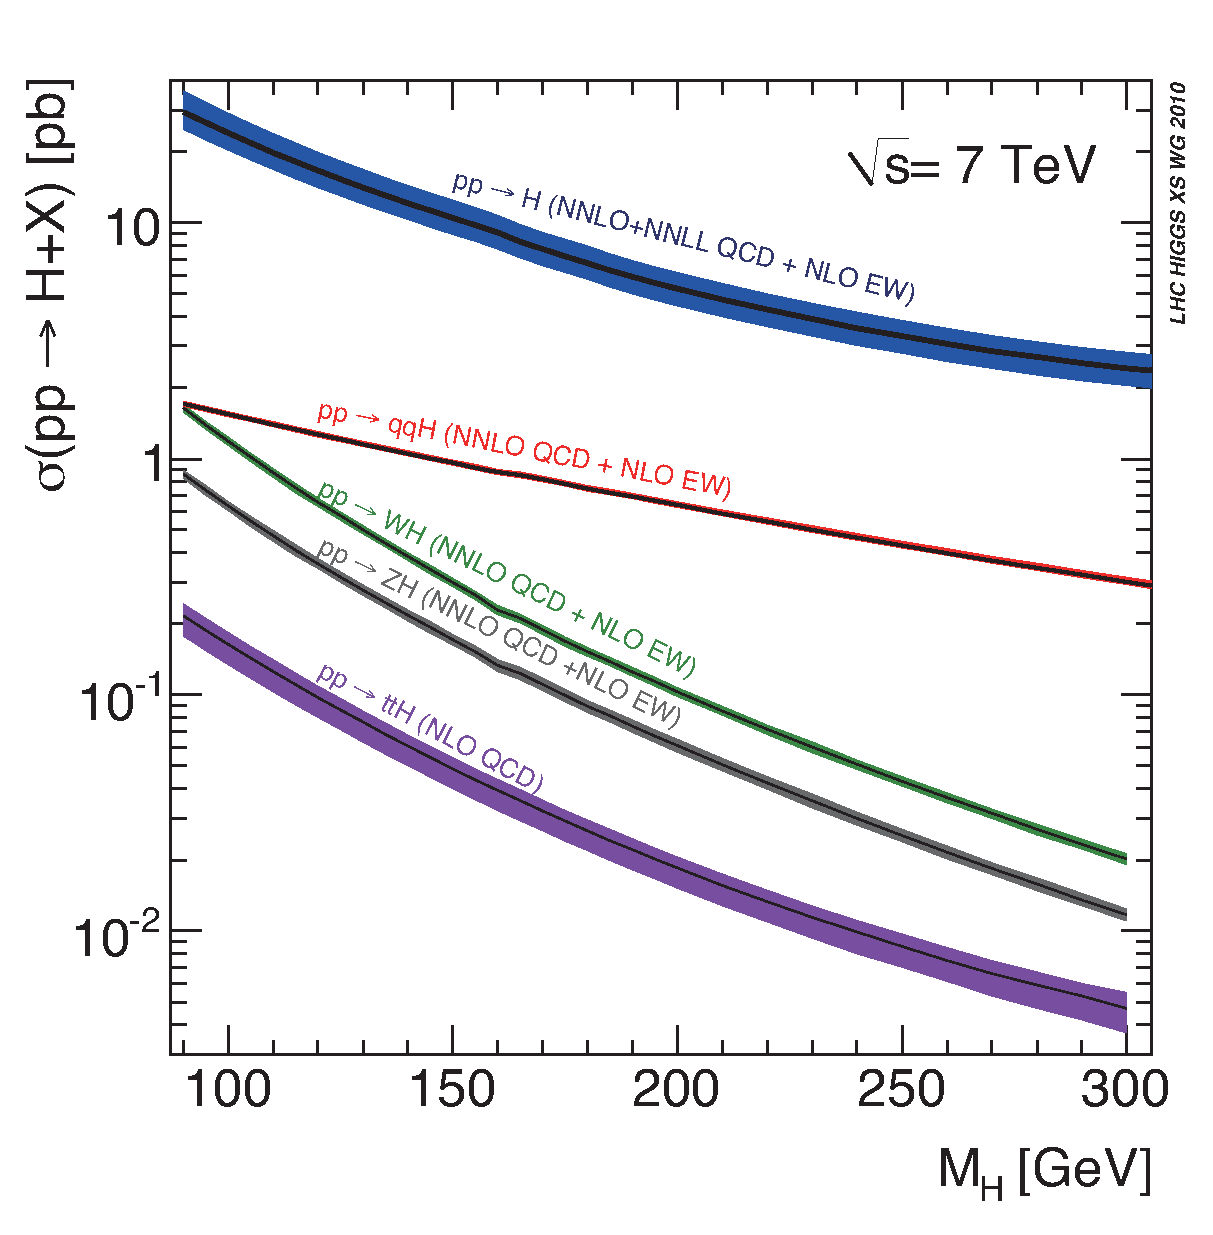
\includegraphics[width=0.48\textwidth]{1_Introduction_Th_and_Exp/pics/Higgs_XS_7TeV_LM.eps}
	\includegraphics[width=0.48\textwidth]{1_Introduction_Th_and_Exp/pics/Higgs_XS_8TeV_LM.pdf}
       \caption{Higgs production cross section at 7 TeV (left) and 8 TeV (right). The bands represent the theoretical uncertainties~\cite{Heinemeyer:2013tqa}.}
       \label{fig:hxs}
\end{figure}


Even though the couplings of the Higgs boson are dictated only by the mass of the fundamental particles, the branching ratio of the Higgs boson to fundamental particles is also dependent on the Higgs mass, as a phase-space factor is added. The dependence of the branching fractions for the main Higgs decay modes as a function of its mass are shown in figure \ref{fig:hbr}. 

\begin{figure}
\centering
\includegraphics[width=0.5\textwidth]{1_Introduction_Th_and_Exp/pics/Higgs_BR_LM.eps}
\caption{Higgs branching ratios for different decay channels as function of the Higgs mass \cite{Heinemeyer:2013tqa}.}
\label{fig:hbr}
\end{figure}

Even though the Higgs boson has no direct coupling to the photon, a seizable branching ratio is given by loop contributions. These loops, as in case of the gluon fusion, could contain contributions from new physics, making this process a viable channel to probe theories beyond the standard model. The branching fraction to down-type fermions, may be sensitive to several beyond the Standard Model (BSM) models, in which these branching fractions are either enhanced or suppressed.

\section{Higgs boson searches}
\label{sec:higgs_res}

On the July 4$^{th}$ 2012, the CMS and ATLAS collaborations reported the observation of a new resonance at the mass of 125 GeV compatible with the SM Higgs boson \cite{Chatrchyan:2013lba}. This observation was based on combining the results of different searches for the Higgs boson in decay channels with gauge bosons, ZZ$^\ast$, WW$^\ast$ and $\gamma\gamma$.

Currently, the significance of the Higgs boson signal exceeds 5$\sigma$ for $\H\To\gamma\gamma$ searches in both CMS and ATLAS \cite{Khachatryan:2014ira, ATLASCONF:2014009}. A similar situation is also present in the ZZ$^\ast$ and WW$^\ast$ channels.

The large amount of signal events in these decay channels has allowed to perform initial studies of the resonance properties. The high invariant mass resolution of $\gamma\gamma$ and ZZ channels has allowed to measure the mass of the boson with high precision: $m_\H = 125.36 \pm 0.37\, \rm{(stat)} \pm 0.18\, \rm{(syst)}$ GeV and $m_\H = 125.03^{+0.26}_{-0.27} \,\rm{(stat)}^{+0.13}_{-0.15}  \,\rm{(syst)} = 125.03^{+0.29}_{-0.31} \, \rm{(tot)}$ GeV for ATLAS \cite{Aad:2014aba} and CMS \cite{CMS:2014ega}, respectively.

The spin and parity ($J^P$) of the resonance has also been studied in the ZZ and WW channels, which are more sensitive to these physical observables. The results, shown in Figure \ref{fig:hjp}, exclude any concurrent hypothesis at more than 99\% confidence level (CL), leaving only $0\+$ as an option \cite{CMS:2014gga}.

\begin{figure}
        \centering
	\includegraphics[width=0.8\textwidth]{1_Introduction_Th_and_Exp/pics/hwwhzz_JP_SummaryPlot.pdf}
       \caption{Summary of different $J^P$ hypotheses tested against the $0\+$ one using ZZ and WW Higgs candidate decays. The orange and blue bands represent the $1\sigma$, $2\sigma$, and $3\sigma$ around the median expected value for the SM Higgs boson hypothesis and the alternative hypothesis, respectively. The black points represent the observed values. }
       \label{fig:hjp}
\end{figure}

The expected SM Higgs boson width for $m_\H \approx 125$ GeV is $\Gamma_\H \approx 4$ MeV, which is below the experimental mass resolution. It has been pointed out that the ratio of on-shell and off-shell Higgs boson production cross section is proportional to the resonance width \cite{Caola:2013yja}; this effect is enhanced in the diboson decay channels by the interference term with the non resonant production. By simultaneously fitting the two contributions it has been possible to measure with better precision the 95\% CL upper limit on the width obtaining $\Gamma_{obs} / \Gamma_\H < 5.3$ for CMS \cite{Khachatryan:2014iha} and $\Gamma_{obs} / \Gamma_\H < 5.7$ for ATLAS \cite{ATLASCONF:2014042}. This method has mild model assumptions, as it neglects the contribution of new physics in the backgrounds and in the gluon-fusion loop. 

The search for Higgs boson decays to bottom quark pairs is the only feasible search to down-type quarks at hadronic colliders, as the coupling to the other two quarks are largely suppressed by their mass while the hadronic background increases dramatically. The large background contamination from heavy-flavor QCD production mandates to search for $\H\To b\bar{b}$ in the experimentally clean production processes such as the associated production with a vector boson, the VBF production, or the $tt$H associated production.
 %restricts the searches to all production processes but the gluon fusion, allowing for the richer final state to be used to remove most of the backgrounds.

The combination of the CDF and D0 results \cite{Aaltonen:2012qt} show a $3.1\sigma$ evidence of the $\rm{H} \To b \bar{b}$ decay mode. The CMS experiment reported a $2.1\sigma$ excess in the VH, $\rm{H} \To b \bar{b}$ production \cite{Chatrchyan:2013zna}, compatible with the SM predictions. The equivalent analysis for ATLAS does not show any excess \cite{TheATLAScollaboration:2013lia}, but is also less sensitive.

The branching fraction of the Higgs boson to muon pairs is predicted to be very low, therefore any excess might be a strong indication of new physics. Both ATLAS \cite{Aad:2014xva} and CMS \cite{CMS:2013aga} have performed a search for  $\rm{H} \To \mu \bar{\mu}$ decays, exploiting the extremely good dimuon mass resolution, without finding any significant excess. The analyses set an independent upper limit on the branching ratio of approximately 7 times the SM expectation.

The SM Higgs coupling to top quarks can only be observed through the $t\bar{t}$H associated production, since the Higgs boson mass forbids the decay of the Higgs into top quark pairs. The search for $t\bar{t}$H \cite{ATLASCONF:2014043,CMS:2014ega} is performed in many Higgs final states. Both ATLAS and CMS exploit the $b\bar{b}$ and $\gamma\gamma$ final states; additionally CMS searches for this production mode also in multi-lepton final states, targeting the $\tau\tau$, ZZ, and WW Higgs decay modes.

The combination of these $tt$H searches leads in CMS to a $3.5\sigma$ excess with respect to the background-only hypothesis \cite{CMS:2014ega}. The combined \emph{signal strength} ($\mu$), i.e. the ratio $\mu = (\sigma \times BR)_{obs} / (\sigma \times BR)_{SM}$, is measured to be $\mu = 2.76^{+1.05}_{-0.92}$, which is two standard deviations away from the SM expectation ($\mu = 1$). The excess in this combination is driven by the same-sign dimuon analysis, which searches for $\H\To \W\W$. The results from ATLAS are consistent with the background-only hypothesis \cite{ATLASCONF:2014043}.

The $\H \to \tau \tau$ decay mode is searched by CMS in gluon fusion, VBF and associated production \cite{H_tautau}. Events are selected in real time by dedicated triggers and according to the isolation of the final state leptons. Events are separated into categories tailored around specific production mechanisms (VBF, VH, gluon fusion) and, in the gluon fusion case, according to the boost of the hadronic tau and Higgs candidates. The invariant mass spectrum of the Higgs final states is smeared due to the presence of neutrinos in the tau lepton decay. To recover this effect, a dedicated likelihood integration method, called SVFit~\cite{Bianchini:2014vza}, calculates the di-tau invariant mass taking as input the momenta of the visible Higgs products plus the information on the reconstructed missing transverse energy (\MET). The mass resolution achieved by SVFit varies between 10\% and 20\%, depending on the final state and the category.

Most of the backgrounds present in the direct production (VBF and gluon fusion) categories are modeled using simulated events with dedicated sideband regions to cross-check the simulation and apply correction factors where needed. The main background for these categories is given by $\Z \To \tau\tau$ events which are modeled with the embedding techniques~\cite{CMS_AN_2011-020}: real $\Z \To \mu \mu$ events are selected from collision data and the two muons are replaced with simulated tau decays.

The search for the Higgs boson in the associated production process is performed in final states including both a Z and a W boson. These searches exploit the presence of the additional leptons in the final state to suppress the backgrounds. The remaining backgrounds are estimated with MC simulation or with the misidentification rate method. Part of the work presented in this thesis has been included in the final result published by the collaboration, but additional effort has been put into estimating the uncertainties in one of the major sources of backgrounds. 

A combined fit to all the channels and categories of the CMS $\rm{H} \To \tau\tau$ analysis reveals a $3.2\,\sigma$ deviation from the background-only hypothesis and a combined $\mu = 0.78 \pm 0.27$. %, well compatible between channels, as shown in Figure \ref{fig:htt_mu}. 
The best-fit mass, $m_\H = 122 \pm 7$ GeV, is compatible with the Higgs mass measured in the ZZ and $\gamma\gamma$ decay channels. The equivalent ATLAS analysis \cite{ATLASCONF:2013108}, which lacks the associated production search, observes a $4.1\,\sigma$ deviation from the background-only hypothesis and measures $\mu = 1.4^{+0.5}_{-0.4}$, which is slightly in excess, but still compatible, with respect to the SM value.

The CMS $\H \To b\bar{b}$ and $\H \To \tau \tau$ searches have been combined leading to a $3.8\,\sigma$ evidence of Higgs coupling to down-type fermions \cite{Chatrchyan:2014vua}.

The result of the single and combined signal strengths for both ATLAS \cite{ATLASCONF:2014009} and CMS \cite{CMS:2014ega} is presented in Figure \ref{fig:combination}.
The outcome of the various searches have been combined by the single experiments in a simultaneous fit in order to determine the couplings of the Higgs boson to the different types of particles. 

\begin{figure}
        \centering
	\includegraphics[width=0.39\textwidth]{1_Introduction_Th_and_Exp/pics/fig_01.pdf}
	\includegraphics[width=0.54\textwidth]{1_Introduction_Th_and_Exp/pics/sqr_mlz_ccc_mH125.pdf}
       \caption{Overview of the different Higgs boson searches performed by ATLAS (left) and CMS (right) with the respective signal strength measured by each channel. The combined result is $\mu = 1.30^{+0.18}_{-0.17}$ for ATLAS and $\mu = 1.00 \pm 0.13$ for CMS.}
       \label{fig:combination}
\end{figure}

Another way to interpret the results is to compute the couplings of the Higgs boson to gauge bosons ($k_V$) and to fermions ($k_F$) and to plot the one-sigma contour regions allowed by each measurement. This interpretation assumes the absence of new physics in loop processes to infer the two couplings from the measurements (e.g. assumes that the gluon fusion is almost completely mediated by a top loop). This interpretation of the results is available in Figure \ref{fig:kvf} for both the experiments.

\begin{figure}
        \centering
	\includegraphics[width=0.53\textwidth]{1_Introduction_Th_and_Exp/pics/fig_05b.pdf}
	\includegraphics[width=0.41\textwidth]{1_Introduction_Th_and_Exp/pics/cVcF_all_channels_2quadrant.pdf}
       \caption{Allowed regions in the $k_V \times k_F$ space as measured by the different Higgs boson searches at ATLAS (left) and CMS (right). The colored contours represent the one standard deviation confidence intervals measured by the different searches and by their combinations. The best fit value of the couplings is marked by the symbol $\times$ (left) and by the black cross (right). The Standard Model point is located at (1, 1) and marked as a black cross on the left and as a yellow diamond on the right. }
       \label{fig:kvf}
\end{figure}

All the results reported so far by both ATLAS and CMS are compatible with the interpretation of the new resonance being a purely SM Higgs boson, but the accuracy of the measurements still allows room for new physics processes.

%In the following part of this work a more detailed description of the $\W\H \To \ell \ell \tau$ analysis will be shown. This 



\chapter{The Large Hadron Collider and the CMS experiment}

This work is based on data collected by the Compact Muon Solenoid (CMS) experiment, 
one of the four main experiments together studying the collisions 
provided by the Large Hadron Collider (LHC). A detailed description of the LHC and of the CMS 
experiment can be found in \cite{Evans:2006tq} and \cite{Chatrchyan:2008aa} respectively.
In this chapter we summarize the main features that are relevant for this work.

\section{The Large Hadron Collider}

The LHC and its experiments were built to explore the high-energy frontier of particle physics and to address fundamental questions of this field such as the existance of a Higgs boson \cite{Englert:1964et,Higgs:1964ia,Higgs:1964pj,Guralnik:1964eu,Higgs:1966ev,Kibble:1967sv}, of extended symmetries \cite{Martin:1997ns}, extra dimensions \cite{Antoniadis:1999bq} or new elementary particles \cite{Beltran:2010ww,Randall:1999vf}. All these phenomena don't have a well-defined energy range predicted by theory even though are expected to manifest at the TeV scale. A proton-proton collider was considered to be the most suitable machine for such a task, allowing higher energies with current technologies and probing wider energy ranges at the same time exploiting the compositeness of the colliding particles.

The LHC is housed in the 27 km long underground tunnel where the Large Electron Positron collider (LEP) has been operating until its decommissioning in 2000. The tunnel is located under both French and Swiss territory, in proximity of the CERN research facility. Before being accelerated in the LHC protons are produced from hydrogen ionization and then accelerated through a chain of smaller machines, some of them dating back to the late 1950's. A schematic view of the CERN accelerators and their connection is shown in Figure \ref{fig:cern_accelerators}. From the last element of this chain, the Super Proton Syncrotron (SPS), protons are injected in the LHC with an energy of 450 GeV in two separate beam pipes, one containing protons running clockwise, the other with protons running in the opposite direction. Protons are bent in their trajectory by 1\,232 superconducting dipole magnets and focused by  superconducting quadrupole magnets, while 16 superconducting radio-frequency (RF) stations 
%provide the thrust to 
accelerate the two beams up to 7 TeV in steps of 0.5 MeV each turn. In order to maintain superconducting properties the magnet coils and the cavities are cooled to 1.9 K by a complex cryogenic system using superfluid helium as refrigerator. RF cavities can be used for accelerating the protons only if the beam is not continuous but structured in bunches. By design the LHC is built to contain 2808 bunches of $10^{11}$ protons each, giving a bunch time separation of 25 ns.
%Due to space constraints both the beam pipes are encased in the same dipole and the proper magnetic field direction is achieved with a particular magnet design.  

\begin{figure}
\begin{center}
\includegraphics[angle=-0,width=0.8\textwidth]{2_LHC_and_CMS/pics/LHC.pdf}
\caption{Schematic view of the CERN accelerators and their connection
\label{fig:cern_accelerators}
}
\end{center}
\end{figure}

The LHC started its operation on 10 September 2008 and after only 9 days of operation a severe \emph{quenching} of about 100 dipole magnets, causing the release of around two tones of helium, forced the machine to stop and to address some design figures. The main cause of the accident was found to be in some of the electrical connections between magnets. In 2009 the machine became again operational with a reduced beam energy, allowing for less current to flow in the dipole magnets. The year 2010, after a careful ramp-up of the beam energies, saw the start of the LHC research program with collisions at a center-of-mass energy $\sqrt{s} = 7$ TeV, half of the designed one. During 2010 and 2011 the machine commissioning continued along with data taking improving the instantaneous luminosity and allowing for an increase of the beam energy to 4 TeV that took place in 2012. The LHC design specifications and achieved ones are summarized in table \ref{tab:lhc_figures}.

\begin{table}[h!]
   \centering
  \caption{Relevant LHC machine parameters. The design values are compared to the ones reached during the 2013 operations.}
\begin{tabular}{c|ccccc}
\hline
Parameter & Design value&  Best value achieved \\ 
\hline
Beam energy   & 7 TeV & 4 TeV \\ 
Number of protons per bunch & 1.15$\times$10$^{11}$ & 1.5$\times$10$^{11}$ \\
Number of bunches & 2808 & 1368 \\
Crossing angle & 300~\si{\micro\metre} & 290~\si{\micro\metre} \\
Beam size & 17~\si{\micro\metre} & 20~\si{\micro\metre} \\
Emittance & 3.75 ~\si{\micro\metre} & 2.4~\si{\micro\metre}  \\
Peak luminosity & $10^{34}$~cm$^{-2}$s$^{-1}$ & 7.5$\times$10$^{33}$~cm$^{-2}$s$^{-1}$ \\
\hline
\end{tabular}
  \label{tab:lhc_figures}                
\end{table}


The instantaneous luminosity,$\operatorname{\mathcal{L}}(t)$, is the number of particles per unit area per unit time available for collisions. For any given physics process the average number events is given by:

\begin{equation} 
	N_{ev} = \sigma\int\operatorname{\mathcal{L}}(t)\mathrm{d}t
	\label{eq:n_events}
\end{equation} 

where $\sigma$ is the cross-section for such process. While the cross section depends on the scattering process, the instantaneous luminosity is entirely derived from accelerator figures:

\begin{equation} 
	\operatorname{{\cal L}}(t) = \frac{N_p^2 n_b f_{rev} \gamma }{4 \pi \epsilon_{n} \beta^*} F
	\label{eq:lumi}
\end{equation} 

where $N_p$ and $n_b$ are the number of protons per bunch and the total number of bunches respectively, $f_{rev}$ is the rotation frequency, $\epsilon_{n}$ and $\beta^*$ describe the beam focusing at the interaction point, $\gamma$ is a relativistic factor and $F$ accounts for the crossing angle between the two beams. Although the number of bunches has always been less than half the design value during all the running period, the peak instantaneous luminosity has been only 30\% lower than the design one. This result was achieved by increasing the number of protons in each bunch and increasing the focusing of the beams, at the price of increasing the average number of proton collisions per bunch crossing, the so-called \emph{pileup}. This effect is displayed in figure \ref{fig:lhc_pileup} where the peak number of simultaneous interactions per bunch crossing recorded by the CMS detector is shown as a function of time.

\begin{figure}
\begin{center}
\includegraphics[angle=-0,width=\textwidth]{2_LHC_and_CMS/pics/peak_pu_pp.pdf}
\caption{Peak Interactions per Crossing versus time for p-p collisions (includes special runs), each point represents a Fill. This is shown for 2010 (green), 2011 (red) and 2012 (blue) data-taking.
\label{fig:lhc_pileup}
}
\end{center}
\end{figure}

The integrated luminosity is usually quoted as \L. During its operations LHC delivered 44.2~pb\Inv in 2010, 6.1~fb\Inv in 2011 and 23.3~fb\Inv at 8~TeV in 2012; Figure \ref{fig:int_lumi} shows the progress of the accelerator in terms of integrated luminosity.

\begin{figure}
\begin{center}
\includegraphics[angle=-0,width=0.8\textwidth]{2_LHC_and_CMS/pics/int_lumi.pdf}
\caption{Cumulative luminosity versus day delivered to CMS during stable beams and for p-p collisions. This is shown for 2010 (green), 2011 (red) and 2012 (blue) data-taking.
\label{fig:int_lumi}
}
\end{center}
\end{figure}


\section{The CMS detector}

The CMS detector is located in the LHC tunnel at point 5, near the French town of Cessy, between the Jura mountains and the Geneva lake.
 
The CMS experiment, together with ATLAS, is one of the two multi-purpose detectors operating at the LHC. Its primary task is to probe particle physics at the TeV scale looking for new phenomena and for the Higgs boson, the only missing piece to the SM puzzle. The experiment is also well suited to perform precision measurements of standard model processes and flavor physics studies. A heavy-ion program is carried on as well to probe QCD at very high energies and matter densities, trying to reproduce an environment similar to the conditions of the universe few instants after the Big Bang.

To carry out such ambitious research program the detector was designed to meet some baseline requirements:
\begin{itemize}
\item Good muon identification and momentum resolution over a wide range of momenta and angles with di-muon mass resolution of ~1\% at 100~GeV.
\item Ability to identify the muon charge without any ambiguity for muons momenta below 1~TeV
\item Good charged-particle momentum resolution, high tracking efficiency and resolution. This two figures are especially important for objects like \b-jets and tau leptons, where isolated charged hadrons and displaced vertices play a fundamental role. A high tracking resolution also plays a key role in assigning the tracks to the production vertex mitigating the effect of pileup.
\item Good electromagnetic energy resolution, with a di-photon invariant mass resolution of \~1\% at 100~GeV and wide geometric coverage with efficient photon and lepton isolation in high pileup conditions.
\item Hermetic hadronic calorimeter with fine transverse segmentation for good jet mass and missing transverse energy ($E_T^{miss}$) resolution. 
\end{itemize}

The total proton-proton cross section at 14~TeV is expected to be roughly 100~mb leading to an average of 20 pileup interactions with LHC design values. This value has been widely overcome during the 2012 data taking. The number of \emph{pileup} events together with the short 25~ns bunch spacing pose stringent requirements on the resolution, granularity and latency of the different subdetectors. The ability to resolve overlapping vertices and assign their respective track is of primary importance. A fast trigger system is also required to reduce the event rate from the design collision rate of 40~MHz to 300Hz which can be permanently stored.

In order to meet all these requirements CMS has been built with a 4~T NbTi superconducting solenoid magnet with an inner diameter of 6 m. Inside the magnet a large silicon tracker, the largest of its kind, is housed to track charged particles with the required resolution. Around the tracker, but still within the solenoid field, a lead-tungstanate electromagnetic calorimeter (ECAL) and a brass-scintillating sampling hadron calorimeter (HCAL) are installed. Inside the 1.5~m thick iron return yoke of the magnet four muon stations are installed. They consist of several layers of drift tubes or cathode strip chambers complemented by resistive plate chambers. A schematic view of a transverse CMS slice is presented in figure \ref{fig:cmsdet}

\begin{figure}
\begin{center}
\includegraphics[angle=-0,width=0.8\textwidth]{2_LHC_and_CMS/pics/CMS_Slice_HD.png}
\caption{transverse slice of the CMS barrel section showing the trajectory for different particles with and the signal deposed in each subdetector.
\label{fig:cmsdet}
}
\end{center}
\end{figure}


\paragraph{The coordinate system}
chosen for CMS sets the $y$ axis vertical pointing upwards and the $x$ axis horizontal pointing towards the center of LHC, therefore the $z$ axis is placed along the beam line pointing in the direction of the beam running anti-clockwise or towards the Jura. An additional set of polar coordinates is used to describe the $xy$ plane in the form of radius $r$ and angle $\phi$, while the angle $\theta$ is measured with respect to the positive $z$ axis direction. Usually the polar angle $\theta$ is replaced by the \emph{pseudorapidity}, defined as $\eta=-\ln \tan(\theta/2)$, is Lorentz invariant for boosts along the $z$ axis and therefore comes very handy when describing processes whose longitudinal boost is unknown. The three-dimensional angular distance is also replaced by its Lorentz-invariant $\D R=\sqrt{\D\phi^2+\D\eta^2}$, where $\D\eta$ and $\D\phi$ are the $\eta$ and $\phi$ coordinate differences of two points.

\subsection{Inner Tracker}
\label{sec:inner_tracker}

The inner tracker provides the essential spatial informations needed to reconstruct charged tracks as well as primary and secondary vertices. A schematic view of the inner tracker is shown in figure \ref{fig:tracker}. To cope with the very high track density and to provide the best spatial resolution, the innermost part of the tracker is based on silicon pixel technology. The pixel detector, displayed in figure \ref{fig:pixel}, is composed of three cylindrical layers at radii of 4.4, 7.3 and 10.2 cm complemented by four disks  in the forward/backward region. The total active area of the pixel detector is roughly of 1 m\sq~and its angular acceptance covers $|\eta| \leq 2.5$, providing three bi-dimensional measurements over the full acceptance. The pixel cell size is 100 $\times$ 150 \u m\sq. High hit resolution is achieved thanks to the sharing of the ionization charge between neighboring pixels due to the solenoidal magnetic field. To enhance this effect in the forward wheels the sensors are placed in a turbine shape. The analogue read-out and charge sharing allow for a 9-33 \u m resolution \cite{trackingpaper}. 

The pixel detector can be extracted from the rest of the tracker to allow easy access for maintenance without interfering with the rest of the detector. This feature is particularly important due to the high radiation dose that the first layers of the pixel detector sustain, requiring additional maintenance.

\begin{figure}
\begin{center}
\includegraphics[angle=-0,width=0.8\textwidth]{2_LHC_and_CMS/pics/trkxsec.pdf}
\caption{Longitunal cross section of the CMS tracker with pseudo rapidity coverage. 
\label{fig:tracker}
}
\end{center}
\end{figure}

\begin{figure}
\begin{center}
\includegraphics[angle=-0,width=0.8\textwidth]{2_LHC_and_CMS/pics/pixelfull.pdf}
\caption{Three dimensional sketch of the CMS pixel detector, barrel modules in blue and endcap wheels in orange.
\label{fig:pixel}
}
\end{center}
\end{figure}

The outer layers of the tracker are made of silicon strip detectors and further divided into four sections: Tracker inner and outer barrel (TIB and TOB), tracker inner disks (TID) and tracker endcaps (TEC), as illustrated in figure \ref{fig:tracker}. TIB and TID are located at radii between 20 and 55 cm from the beam line. They consist of four barrel layers and three disks at each end. The sensors are made of 320 \u m thick silicon with a strip pitch that varies from 80 \u m in the innermost barrel layer to 140 \u m in the outermost disks. The combination of TIB and TID delivers up to four transverse measurements. The TIB-TID sections are surrounded by the TOB, which fills the remaining space up to a radius of 116 cm from the beam line. It consists of six barrel layers of 500 \u m thick sensors with a strip pitch of 183 \u m for the first four layers and 122 \u m for the remaining two. The TEC is located in the end-cap region, for radii larger than 20 cm and $|z| > 118$ cm. It consists of nine disks composed by up to seven concentric rings of strip sensors. The thickness and the strip pitch of the sensor vary depending on the distance from the beam line. 

Intrinsically strip sensors only provide one dimensional spatial information ($\phi$). To measure a second coordinate ($r$ for disks, $z$ for barrel), an additional set of sensors is mounted back-to-back with a stereo angle of 100 mrad on the first two layers of TIB, TID and TOB and on layers 1, 2 and 5 of TEC. The strip tracker layout ensures about 9 hits in its acceptance with at least four of them being two-dimensional.

%temperatura?

\subsection{Electromagnetic Calorimeter}

The CMS electromagnetic calorimeter (ECAL) is located around the inner tracker. It is divided into ECAL Barrel (EB) covering the pseudo rapidity range $|\eta| < 1.479$ and ECAL Endcaps (EE) which cover $1.479 < |\eta| < 3$. 
The calorimeter consist of 68\,524 scintillating lead tungstanate (PbWO$_4$) crystals readout by photomultipliers. 

The choice of lead tungstanate was driven by its high density yielding a short radiation length (0.89 cm) and small Moliere radius (2.2 cm) together with the radiation hardness and fast response, with 80\% of the light yield emitted within 25~ns. To keep the calorimeter as hermetic as possible the crystals have truncated pyramidal shape with one of the longitudinal faces left unpolished to moderate the non uniform light collection across the crystal length that this peculiar shape causes. Each crystal covers about $0.0174 \times 0.0174$ in $\eta-\phi$ plane and is oriented pointing towards the nominal interaction point with a slight misalignment to mitigate the effect of the crystal surface on photon detection. Each crystal is read-out by either a pair of avalanche photodiodes (APD) in the barrel or by vacuum phototriodes in the endcap. Both the devices can operate in high magnetic fields with little or no efficiency degradation and showed good radiation resistance.

A pre-shower detector is installed in front of the ECAL endcap, with the purpose of discriminating between real photons and in-flight \piz decays and to enhance the angular resolution of both electrons and photons. The pre-shower detector consists of a double-layer lead-silicon calorimeter, with the lead initiating the shower and the silicon strip detector placed after each radiator measuring the deposited energy and shower profile with high granularity.

\subsection{Hadronic Calorimeter}

The hadronic calorimeter (HCAL) serves two purposes: it measures the energy of charged and neutral hadrons from the p-p interaction while stopping them, thus allowing only muons to pass through and avoiding large quantities of energy being deposited inside the superconducting magnet. As most of the other subdetectors HCAL is divided in a barrel section (HB), covering the acceptance region with $|\eta| < 1.3$, and an endcap section (HE) covering $1.3 < |\eta| < 3$. Both parts are located inside the superconducting solenoid. HCAL is a sampling calorimeter with brass passive plates, in which the hadronic shower begins and develops, interspaced with active plastic scintillator measuring the shower profile and the energy deposited. 

The scintillator is segmented both in $\eta$ and $\phi$ to provide the necessary granularity. Each scintillating tile is connected to the readout by a wavelength-shifting fiber that runs in a groove machined in the tile itself. Such fiber is thermally spliced to a clear fiber carrying the emitted light to a hybrid photodiode (HPD). The HPDs consist of a photocathode kept at high voltage. Electrons emitted by the photocathode are accelerated in the short distance (\~3 mm) that separates the cathode from a silicon pixelated anode which amplifies the signal. These devices were chosen due to their high dynamic range, their high gain ($O(2000)$) and the possibility to work in a magnetic field.

The effective thickness of the calorimeter in terms of interaction length, $\lambda_I$, spans in the barrel from a minimum of 5.82 $\lambda_I$ at $\eta=0$ to a maximum of 10.6 $\lambda_I$ at $|\eta| = 1.3$. The ECAL crystals add about 1.1 additional interaction lengths. The total thickness of the endcap calorimeters, including in the ECAL crystals, is about 10 $\lambda_I$.

Due to the limited stopping power of HB, especially in the central rapidity region, an additional hadronic calorimeter is placed outside the solenoid magnet (hadron outer or HO) with the function of \emph{tail catcher}. The HO consists of one scintillating station (two for the most central region) exploiting the solenoid itself ( and the first return yoke in case of the second station) as absorber. This additional detector extends the total thickness of the HB to a minimum of $11 \lambda_I$.

\subsection{Muon System}

Muon detection and trigger are of prime importance in CMS as many new physics processes may manifest through decay chains involving muons. Among those, the decay of a Higgs boson into $\Z\Z^*\To4\mu$ stands out as one of CMS's flagship analyses and one of those leading to the discovery of the Higgs boson announced on July 4$^{th}$, 2012 \cite{Chatrchyan:2013lba}. For this reason a redundant system of three different kinds of detectors is used to track muons in CMS. 

The muon system, whose scheme is shown in figure \ref{fig:mudet}, is housed in gaps between the return yoke of the solenoid magnet in the outermost region of the experiment. It consists of a Drift Tube (DT) tracking system in the barrel and multi-wire proportional chambers in the end-cap. In addition, a set of Resistive Plate Chambers (RPC) is located both in the barrel and in the endcap regions, providing a better time resolution  at the cost of coarser spatial resolution. 

\begin{figure}
\begin{center}
\includegraphics[angle=-0,width=0.8\textwidth]{2_LHC_and_CMS/pics/mudet.pdf}
\caption{Longitudinal cross-section of the CMS detector showing the location of the muon system.
\label{fig:mudet}
}
\end{center}
\end{figure}

\subsubsection*{Drift Tubes}

Drift tubes identify and track muons in the barrel region ($|\eta| < 1.2$) where the rate is below 1 Hz/cm\sq ~and residual magnetic field less than 1 T allowing the usage of this technology. Four stations are located at increasing distance from the beam line. The first three stations are equipped with two \emph{super-layers} (SL) providing a measurement of $\phi$ and one SL measuring the $z$ coordinate, as can be seen in figure \ref{fig:dt_module}, representing one DT module. In the last two stations the SL measuring the $z$ coordinate is missing. 

\begin{figure}
\begin{center}
\includegraphics[angle=-0,width=0.8\textwidth]{2_LHC_and_CMS/pics/cms_dt.png}
\caption{Cross-section view of a DT module.
\label{fig:dt_module}
}
\end{center}
\end{figure}


Each SL is made of four stacked layers of tubes staggered by half a cell. This configurations eliminates blind spots and allow for an easy measurement of the muon crossing time by averaging the drift times. Each tube has a rectangular cross-section of $13\times42$ mm\sq ~and is filled with a gas mixture of 85\% Ar and 25\% CO$_2$, leading to a maximum drift time of 380 ns. Each SL has a spatial resolution of about 200 \u m and a time jitter below 5 ns.

\subsubsection*{Cathode Strip Chambers}

The front wheels of the solenoid return yoke are instrumented with multi-wire proportional chambers. Each module has trapezoidal shape and cover either $10\deg$ or $20\deg$ in $\phi$ forming a full disk perpendicular to the beam axis ($r-\phi$ plane). Each of these chambers has the cathode segmented radially in strips (hence the name Cathode Strip Chamber, CSC) of constant $\Delta\phi$ and wires running perpendicular to the strips with spacing of 3.2 mm. 

This design allows to cope with the much higher rate with respect to the barrel and with non uniform and non null magnetic field. 

This detector provides at least three measured points in its acceptance ($1.2 < |\eta| < 2.4$) with a design resolution of approximately 2 mm at trigger level and around 200 \u m after offline reconstruction.

\subsubsection*{Resistive Plate Chambers}

Dual-gap RPC's provide a redundant set of spatial measurements particularly important for trigger purposes, given their response time much shorter than 25~ns. The layout chosen by the CMS collaboration consist of six RPC stations in the barrel and three in the endcaps. RPC stations are placed in proximity (before or after) each CSC or DT station. The first two DT station have two RPC, one before \emph{and} one after, in order to provide at least four position measurements even for low-$p_T$ muons which might not reach the outer stations. Each chamber is operated in avalanche mode and consist of two gaps sharing a segmented pick-up read-out in between, allowing to operate at lower voltages (and therefore lower noise) for the same gain. 

\subsection{Trigger}

As previously said, during the operations LHC delivered an interaction every 50 ns leading to a 20 MHz frequency, half of the design one.
This frequency is well above the storage capabilities of the most modern technologies that allow to accommodate few hundreds of events per second. The inclusive p-p cross-section is hugely dominated by low-$x$ QCD processes that are of no or little interest for this experiment. This leads to the obvious necessity of a fast-logic to isolate events of some interest for the experiment's physics program while rejecting the others. This event selection of logic, usually referred as \emph{trigger}, is divided in the CMS experiment in two stages: the \emph{level one} (L1) trigger and the \emph{high level trigger} (HLT). 

The L1 trigger decision is based on a coarse reconstruction of the event performed by custom electronics largely mounted directly on the detector. The maximum processing time (called \emph{latency}) is 3.2 \u s. During this time the event is stored on the detector electronics in pipelined memories. Due to timing constraints only inputs from the calorimeters and from the muon system are processed. In this trigger process, the calorimeter segmentation is reduced into the so-called \emph{trigger-towers}. Calorimeters provide to the decision logic a set of important physics variables like the missing transverse energy ($E_T^{miss}$), the scalar sum of the transverse hadronic activity ($H_T$), the number of jets above different energy thresholds and the locations of towers compatible with a \emph{minimal ionizing particle} (MIP) and its isolation. Electron and photon identification is also performed looking at the jet hadronic over electromagnetic energy ratio ($H/E$) and cluster shape, performed with the aid of a look-up table. Muon information is mainly provided by DT and CSC subdetectors complemented by the sheer time resolution of RPC for bunch crossing assignment as well as ghost-tracks removal. Muons trajectories are roughly reconstructed by the detector dedicated electronics and then sent to an additional module that merges the information coming from the different stations and subdetectors to assess the transverse momentum  and charge. These informations are complemented by those coming from the calorimeters providing isolation values.

The final decision is taken by modules located outside the detector. These modules exploit FPGA's to achieve fast response while allowing for modification of the algorithms to cope with the evolution the instantaneous luminosity or new physics demands. The maximum output frequency for L1 is 1 kHz.

Once the L1 trigger decision is made the full event is read out from the detectors buffers and sent to the online \emph{Data Quality Monitoring} (DQM) and to the HLT farm, consisting of over a thousand commercial processors working in parallel. During the HLT decision, a simplified version of the CMS offline event reconstruction is performed. Time consuming tasks such as tracking are performed only around the objects that caused the L1 trigger to fire and more complex algorithms like \b-tagging and \t~identification are performed with a simplified version. During this trigger stage, decisions are taken on the basis of more complex algorithms and a more refined reconstruction, which allows to reduce the event rate to roughly 300Hz, within the storage and processing capabilities of the CERN facilities. Being completely software-based, the HLT is far more flexible and fast evolving than the L1 trigger, allowing to cope with the fast changing machine conditions during 2010 and 2011 runs and achieving a level of refinement beyond the most optimistic forecasts made at the start-up.

Once the event is accepted by the HLT too, it is transferred to the CERN computing center for storage and reconstruction.

\section{Data storage and processing}

Events recorded from the detector are stored in \emph{RAW} format, a data format that contains all the digitalized output of the single subdetectors and L1 and HLT information. In order to be useful for physics analysis the trajectory and the nature of the particles originated in the event must be inferred from the hits stored in the RAW event. This process is usually called event reconstruction and is the topic of the following chapter. The CMS detector produces about 15 TB of data for each day of operation.

The reconstruction of collected and simulated data is too CPU and storage demanding to be delegated to a single facility. In order to evenly spread this effort through different computing facilities in various parts of the world, a new computing model has been created. The \emph{world wide computing grid} \cite{Malecki:2005gn} allows for fast transfer and de-localized computing throughout the world, allowing to cope with the huge demands that the LHC experiments need to smoothly operate. 

In some sense the grid can be seen as an extension of the batch queue system where the user submits jobs to a single machine, whereas, in this case, he submits them to clusters of machines, that then take care of submitting those jobs in their peculiar batch queue implementation. Computing facilities are organized in a hierarchical structure called tiers, starting from the facility that receives the data from the detector, called Tier0, scaling to smaller and smaller facilities up to Tier3's which provide limited computing and storage for local groups. In this system secure access to the resources is ensured by a system of certificates spawning children proxies of limited lifetime.

%displayed
%presented
%illustrated
\chapter{Event reconstruction in CMS}

During physics collisions at LHC particle traversing the different layers of sub-detectors deposit some energy in them that gets amplified and recorded by the detectors themselves. Most of the detector measure the particle position as well as the energy deposited in them. Each event therefore results in a series of dots in the different layers of the tracking detectors and in large energy clusters in the calorimeter. The reconstruction algorithm takes care of ``connecting the dots'' and return the most complete and accurate description of the event as it originated from the collision. In this game CPU time also plays an important role, as the algorithms used by the reconstruction cannot be excessively resource demanding and be the bottleneck of physics analyses. In this chapter we will briefly describe the techniques used to reconstruct the events recorded by the CMS detector starting from the most basic objects and then moving forward most complex ones finally describing the \emph{Particle Flow} algorithm that aims to give a global description of the event.

\section{Track reconstruction}

The signals recorded by the innermost sub-detector, the inner tracker \ref{sec:inner_tracker}, are used to reconstruct the trajectory of all the charged particles originating from the proton collisions as well as the location (vertex) where these interactions occurred inside the beam pipe. An accurate and detailed description of the tracking algorithm may be found here \cite{cms_trk_11_01}.

The innermost part of the tracker, made of pixel detectors, records the hit position together with the charge deposited in the detector and the cluster shape. Due to the lorentz drift the charge of a traversing ionizing particle is in fact shared between neighboring pixels, improving the position resolution on the hit. The outer part of the tracker, made of strip detectors, records only the $\phi$ coordinate of the impact except for few layers where an additional layer of strips rotated with a 100 grad stereo angle provides an additional coordinate at the price of creating possible ghost hits.

Due to huge number of hits recorded in each event, reconstructing the track from the hits on the detectors is a hard challenge. The strategy adopted by the CMS collaboration consist of running a simple \emph{combinatoric track finding} (CTF) with very stringent requirements on the tracks to be found, thus finding the easiest tracks. These requirements are loosened in several iteration, after which the hits used to build the tracks are removed from the pool of available hits. This procedure, called \emph{iterative tracking}, allows to keep a very high tracking efficiency with low fake rate and limited resource usage. 

At the beginning of each iteration the tracks are seeded from triplets or doublets of hits in the tracker. In case of doublets an additional constraint of the beam-spot is used to reduce the fake rate. Only 2D hits are used in this stage to build track seeds. A first evaluations of the main track parameters (\pT and 3D impact parameter) is also performed at the seeding step, track seeds not respecting the minimal requirements for that iteration are discarded.

Track seeds are then propagated in and outwards the seeding layers in search for compatible hits to assign to the track. The analytical propagator used at this stage assumes uniform magnetic field in between the two detector layers and neglects multiple scattering effects. New candidate hits are added to the track candidate and its parameters are updated by a \emph{Kalman Filter} \cite{Fruhwirth:1987fm}. Only the track candidates satisfying a certain quality of the fit (evaluated with the $\chi^2$) are retained. This process, known as \emph{track finding}, is repeated until to the innermost and outermost layer of the tracker is reached by the track propagation. During this process the Kalman Filter retains only the latest and most accurate evaluation of the track candidate parameters and the addition of a new hit does not require re-evaluating the full trajectory from scratch, saving a large amount of computing time. Track candidates emerging from this process are cross-cleaned agains each other, merging those candidates sharing the majority of the hits. Mutually-exclusive hits (hits belonging to the same detector layer) are arbitrated according to the goodness of the $\chi^2$ of the track fit.

Track candidates found during the track finding step are then fitted by the means of Kalman filter and smoother, this choice turns out to be as accurate as a standard fit, but is more computing effective. Trajectory parameters are evaluated both starting from the innermost hit in the tracker and from the outermost one and then averaged, avoiding any bias due to the recursive nature of the Kalman Filters. During this process the more refined Runge-Kutta propagator is used to take into account un-uniformities of the magnetic field and the effect of material. Track candidates are finally selected according to the quality of the fit. Hits belonging to the tracks produces by this last step are removed from the collection of hits available for building tracks and a new iteration with different seeding conditions and track requirements begins. 

A total of six iterations is performed on each event, the first ones are aimed to reconstruct most of the tracks originating from the main vertex, while the following ones focus on reconstructing tracks coming from displaced decays of long living particle and from vertices in peripheral areas of the interaction region.

The solution adopted for the track reconstruction allows for a tracking efficiency higher than 90\% over a wide region of the \pT spectrum.

\paragraph{Muons} can be considered a special case of the tracking algorithm given the dedicated muon tracking system located outside the solenoidal magnet. This additional lever arm allows to keep a very good momentum resolution above 200 GeV, where the tracker resolution begins to degrade. In CMS muon candidates can be seeded both from the tracker or form the muon chambers. In the former case every track above few GeV is considered a potential muon and a tentative match with hits in the muon stations is performed. If the match succeeds, the track is refitted and it aquires the status of \emph{tracker muon}. In the latter approach, a track segment reconstructed in the muon chambers is propagated inside the tracker to match with a track. As with the previous method, a positive match causes the full trajectory to be refitted and the object is considered a \emph{global muon}. Tracker muon reconstruction is obviously more efficient than the other for low \pT muon since they may not leave enough hits in the muon chambers to preform a full track reconstruction, but they also suffer of a much larger fake rate. The two muon collections are then merged into a single one, removing double candidates.

\section{Vertex reconstruction}

Vertices are reconstructed in CMS through a \emph{Deterministic Annealing} (DA) \cite{IEEE_DetAnnealing} clustering algorithm. Tracks used during the vertices reconstruction are preselected according to their transverse impact parameter from the beam spot, the number of hits on the tracker and the $\chi^2$ of the track fit, to ensure that only good tracks coming from the proton collisions are used in the latter stages. No requirement on the \pT of the track is imposed to allow the reconstruction of minimum bias events with high efficiency.

Once the tracks are selected any further computation is based on the $z$ coordinate of the points of closest approach of the tracks with respect to the beamspot ($z_i^T$) and its uncertainty ($\sigma_i^Z$). In the DA framework the vertices positions are evaluated by minimizing a modified version of the $\chi^2$ with an additional term artificially inflating $\sigma_i^Z$ of each track. This parameter is called ``temperature'' since it exactly behaves like the physics observable in statistical mechanics, with the  $\chi^2$ acting as free energy.

Starting from one single located centrally, the temperature is iteratively lowered and the free energy term minimized for each iteration. As the temperature lowers, some tracks will start being incompatible with the single vertex available and a better minima will be found by splitting the tracks in two sub-sets belonging to two different vertices. This splitting is done ``softly'' as each track can be assigned to multiple vertices with a weight between 0 and 1. With the lowering of the temperature such weights will tend to assume values closer and closer to the end-points.

The annealing process is continued down to a minimal temperature, which is a compromise in vertex resolution and the risk of splitting true vertices. After this threshold no more splitting are allowed, but the temperature is still iteratively reduced and posseble outliers in the vertex fits are removed. After the final temperature ($T=1$) is reached, tracks are assigned to the belonging vertices if their weight to such vertex is greater than 0.5 as spurious weights may still be different from zero. 

Each set if tracks assigned to a vertex is then fitted with the \emph{adaptive vertex filter} algorithm \cite{CMS_NOTE_2007-008}, cons isting of an iterative weighted Kalman Filter, to evaluate the vertex position with the best possible precision.

Such refined technique allows to achieve a vertex reconstruction efficiency between 98\% for cluster  of two or three tracks and 100\% for the rest, with a negligible fake rate of about 1\%. The vertex resolution is found to be of the order of roughly 200 \um both in the transverse and longitudinal plane for clusters of few tracks, rapidly decreasing to an asymptotic value of about 20 \um as more tracks are used to compute the vertex position.

\section{Electron and Photon reconstruction}

Both electron and photon are reconstructed starting from ECAL clusters, which are seeded from local maxima in the energy deposition. A cluster size of $5\times5$ crystals contains on average 95\% of the energy of an unconverted photon. The material in front of the calorimeter, increasing the chafes of a photon conversion, and the magnetic field, bending the charged conversion products in the $r-\phi$ plane, reduce considerably this value for the average of the photons and spread the energy deposits in wider strip in $\phi$. Similar arguments can be made for electrons and positrons, that leave a trace of \emph{bremsstrahlung} photons as they approach the surface of the calorimeter. In order to recover this energy the $5\times5$ clusters are grouped together in \emph{superclusters} (SC) stretching in the $\phi$ coordinate, a more detailed description of the clustering algorithm can be found in \cite{CMS:2006tdr1}.

The bremsstrahlung process and its intrinsic non-gaussian energy emission makes the Kalman filter approach used by the tracking unsitable and is substituted for the dedicated tracking by the Gaussian Sum Filter (GSF) \cite{gsf} with handles the energy loss properly. The usage of the GSF and its larger propagation uncertainties makes a tracker-only approach unfeasible both for CPU consumption and for low track purity. In order to reduce the amount of fake tracks the seeding step starts from the ECAL superclusters that are propagated inside the tracker under both charge assumption to find two compatible hits in the pixel detector. After the seeding the tracking process continues as described in the previous section with the GSF substituting the KF. This modified version of the tracking algorithm is also used to correctly identify photon conversions in the tracker itself, looking for highly displaced vertices compatible with a null invariant mass and matching a broad supercluster in the electromagnetic calorimeter.

Several input variables are used to discriminate between fake and real electrons, addressing the supercluster shape and its energy and location with respect to the reconstructed track parameters along with the presence of energy deposits in the hadronic calorimeter. All these variables are combined to perform an identification. Several working points, both with cut-based and MVA-based approach are available.

Photon identification is based on substantially the same supercluster quantities as the electron identification and the lack of tracks matched to the ECAL deposit.  

\section{Particle Flow}


Particles originating from the proton-proton collisions and traversing the CMS detector are expected to yield a signal in multiple sub detectors. This redundancy is exploited by the \emph{Particle Flow} (PF) algorithm to improve the over-all description of the event. This method also allows for cross-cleaning spurious deposit and achieve a global description of the event.

Building blocks for the PF algorithm are the track collections from the different methods (CTF, GSF, and muon) and calorimeter deposits. Local maxima in the calorimeter deposits serve as seed for ``topological clusters'' that are grown by iteratively adding adjacent cells with an energy deposit above a customizable threshold. After the clustering stage the algorithm liks the different blocks according to their position in the $\eta-\phi$ plane. Tracks are considered linked to calorimeter clusters if the track trajectory propagated to the average shower depth into the calorimeter falls within the cluster boundaries, slightly extend ended to account for uncertainties. Calorimeter clusters are considered to be linked if the center of the cluster of the calorimeter with best granularity falls within the boundaries of the other cluster, the hierarchy is the following: pre-shower, ECAL, HCAL. After the linking step is completed the algorithm starts building the final objects, starting from muons. Each global muon with a combined momentum measurement compatible with the tracker only one gives rise to a \emph{PF muon}. The corresponding track is removed from the collection of tracks and an estimate of the energy deposit in the calorimeters is also removed from linked clusters. Electrons are the second kind of objects to be built with the procedure explained in the previous section of this chapter. Tangents from the electron trajectory in correspondence of the tracker layers are propagated to the ECAL in search for bremsstrahlung photons. If the electron candidates passes the reconstruction a \emph{PF Electron} is created and the track and all the ECAL deposits linked to it are removed. A tighter selection is performed on remaining tracks, requiring that the tracker \pT resolution is smaller than the calorimetric energy resolution. This requirement is found to reject about 0.2\% of tracks in hadronic jets, 90\% of which being fake tracks. Nonetheless this requirement was found to be a issue for hadronic tau reconstruction for high \pT taus and a custom modification was introduced. The algorithm finally exploits the redundancy in the transverse momentum measurement performed by the tracker and by the calorimeter to build \emph{PF charged hadrons, photons and neutral hadrons}. Photons and neutral hadrons are in fact produced out of the calorimetric energy in the clusters once the energy of the incoming tracks is subtracted. PF works under the assumption that all the hadrons (charged and neutral) traversing the detector are pions. In the rare case that a calorimetric cluster has a total energy that is incompatible and lower than the sum of the linked tracks a dedicated procedure aimed at recovering mis-reconstructed muons is performed, recovering muon identification efficiency at no expense in the fake rate. Finally, to each PF object is assigned a PDG identification number and a mass according what the algorithm has inferred.

\subsection{Muon Identification}

A muon identification is necessary in order to suppress the hadronic punch-through and the decay in flight of pions, this work uses the tight working point of the muon identification provided by the Particle Flow algorithm.
To pass the PFTight identification working point a muon candidate must fulfill the following requirements:

\begin{itemize}
\item It must be reconstructed as global and PF muon
\item The normalized $\chi^2$ of its global track fit must be less than 10
\item There must be a least one muon chaber hit included in the global fit
\item At least two muon stations must be matched to the candidate
\item Its tracker track must have a transverse inpact parameter $\mathrm{d}_{xy} < 2$ mm and a longitudinal distance $\mathrm{d}_{xy} < 5$ mm
\item It must have at least one hit in the pixel detector and more than 5 hits in the whole tracker
\end{itemize}

\subsection{Isolation}

A large fraction of the leptons produced in a proton-proton collision come from the decay of mesons inside jets. In order to separate the ones truly coming from the decay of a heavy resonance is important to quantify the \emph{isolation} of the lepton, i.e. the amount of hadronic activity surrounding the lepton trajectory in a cone of defined \DR. The isolation can be divided into its charged and neutral components. 

While the effect of pileup can be easily removed from the charged isolation by requiring that this value is computed accounting only for tracks coming from the selected primary vertex, the same cannot be said for the neutral one. In fact calorimeters don't have enough resolution to assign to each cluster the belonging vertex. The contribution to the neutral isolation form pileup is estimated by computing the charged isolation from pileup and correcting it for a factor 2:1 to account for the amount of neutral energy with respect to charged one. This estimate is called \emph{$\Delta\beta = I^{pileup}_{charged}/2$}. To limit the effect of statistical fluctuations in the charged to neutral ratio on event-by-event basis the $\Delta\beta$ correction is capped to the neutral isolation value. The \emph{relative isolation}, i.e. the isolation divided by the \pT of the object, can be therefore written as.

\begin{equation}
I_{rel} = \dfrac{I_{abs}{\pt}  \dfrac{\sum{p_{T charged}} + \operatorname{max}(\sum{E_{T neutral}} - \Delta\beta, 0)}{p_T}
\label{eq:db_rel_iso}
\end{equation}

\subsection{Jet clustering and missing transverse energy}

Particle flow object are clustered using the \emph{Anti-kT} \cite{Cacciari:2008gp} algorithm. The Anti-kT belongs to the family of sequential recombination algorithms together with the Cambridge-Aachen and kT algorithm. All these algorithms to operate need a definition of distance between two objects (in this case PF ones) and a distance from the beam. In the Anti-kT, the distance between two objects is defined as:

\begin{equation}
d_{ij} = \operatorname{min}(\dfrac{1}{p_{Ti}^2},\dfrac{1}{p_{Tj}^2})\dfrac{\Delta R_{ij}^2}{r^2}
\end{equation}

where $r$ is a constant parameter defining the size of the jet cone.
The distance of an object from  the beam is defined as:

\begin{equation}
d_{iB} = \dfrac{1}{p_{Ti}^2}
\end{equation}

The algorithm starts with a high-\pT object used as seed and then it clusters around all the object until the minimum distance between the candidate jet and the closest object is greater than $d_{iB}$. One can show that this algorithm is infra-red safe, meaning that the jet shape and energy don't depend strongly on the soft energy clustered around hard probes. The Anti-kT algorithms gives rise to almost-conical jets of size $r$ in angular aperture, special cases are overlapping jets and jets with multiple hard probes within the angular acceptance.

Jets used in this work have been reconstructed with the Anti-kT algorithm with a radius of 0.5 and their energies have been corrected to account for non-linear response of calorimeters and other instrumental effects \cite{Chatrchyan:2011ds}.

Pileup interactions deposit a considerable amount of energy in the detector, this energy can easily overlap among different vertices and be misinterpreted by the Anti-kT algorithm as one hard jet. The CMS experiments exploits a combination of tracking and jet shape variables to discriminate between pileup jets and jets coming from the hard scattering. The information provided by these variables is interpreted by \emph{boosted decision tree} \cite{CMS-PAS-JME-13-005} trained on simulated $\Z\To\mu\mu$. The training is divided in four different $|\eta|$ categories that reflect the resolution of tracking information and granularity of the calorimeters.

\paragraph{Missing transverse energy}

Most of the particles produced in a p-p collision leave a signal in at least one sub-detector except neutrinos and other hypothetical weakly interacting neutral stable particles. Even though these particle leave no trace in the detector their presence can still be inferred in the transverse momentum imbalance of detected particle. This observable is called \emph{missing transverse energy} (\MET) and the one used in this work is computed as the negative vectorial sum of all the PF objects reconstructed \cite{CMS-PAS-JME-13-003}. 

\begin{equation}
\vec{\cancel{E}_T} = -\sum \vec{p_{T}}
\end{equation}

The magnitude of this \MET is found to be underestimated for various reasons including thresholds in the clustering of deposited energy and non-linearities in the response of the calorimeters. This bias is significantly reduced when the correction to jet energies is introduced to the formula \cite{Chatrchyan:2011ds}, obtaining the ``type 1''-corrected \MET.

\begin{equation}
\vec{\cancel{E}_T^{corr}} = \vec{\cancel{E}_T } - \sum_\mathrm{jets} (\vec{p}_\mathrm{T,jet}^\mathrm{corr}-\vec{p}_\mathrm{T,jet}),
\label{eq:Type1MET}
\end{equation}

Additional corrections, named ``type 0'' and ``$\phi$'', correct for biases induced by pileup and by asymmetries in the $\phi$ direction.

\section{Tau reconstruction and identification}

Hadronic taus are one of the highest level objects reconstructed in the CMS detector and the last in the reconstruction chain. The reconstruction and identification algorithm exploits all the capabilities of the detector and of the Particle Flow algorithm to achieve a reconstruction efficiency close to 60\% with a sub-percent fake rate. The tau reconstruction algorithm used in CMS is called \emph{Hadron Plus Strip} (HPS) \cite{CMS-PAS-TAU-11-001}. 

\subsection{Reconstruction}

Tau reconstruction is seeded from PF jets clustered with Anti-kT algorithm and radius of 0.5. In order to recover most of the photon conversions, PF electromagnetic objects (electrons and photons) with deposited energy above 0.5 GeV are clustered in topological ``strips'' $0.05 \times 0.20$ wide in $\eta$ and $\phi$ respectively. Strips satisfying a minimum transverse energy of 2.5 GeV are combined with the charged hadrons to form the tau candidate. Charged hadrons involved in the tau reconstruction are required to satisfy the following requirements:

\begin{itemize}
\item $\pt > 0.5$ GeV
\item track $\chisq < 100$
\item track transverse distance of closest approach to the PV $d_0 < 0.03$ cm
\item track longitudinal distance of closest approach to the PV $d_z < 0.4$ cm
\item At least three hits in the tracker
\end{itemize}

The algorithm proceeds to build all possible combinations of hadrons and strips matching one of the four decay modes accounted for:

\begin{enumerate}
\item \emph{single hadron}: corresponding to one single hadron and no strips
\item \emph{hadron plus one strip}: the invariant mass of the pair has to fall within the window of the $\rho$ meson, $0.4 < M_{\tau} < 1.3 \cdot \sqrt{\pt \mathrm{[GeV]} / 200}$ GeV. The upper boundary of this window is limited at 1.3 (2.1) GeV for candidates with $\pt < 200 \, (> 800)$. This shifting window size compensates for resolution effects at high \pT.
\item \emph{hadron plus two strips}: the invariant mass of the triplet has to fall within the window of the $\rho$ meson, $0.4 < M_{\tau} < 1.2 \cdot \sqrt{\pt \mathrm{[GeV]} / 200}$ GeV. The upper boundary of this window is limited at 1.2 (2.0) GeV for candidates with $\pt < 200 \, (> 800)$.
\item \emph{three hadrons}: the invarian mass of the triplet must fall within the window of the $a_1$ meson, $0.8 < M_{\tau} < 1.5$ GeV. The tracks are required to be compatible with originating from the same vertex and to sum to unit charge
\end{enumerate}

In addition the previous requirements, tau constituents are required to be contained in a cone of size 0.1, $3 / \pt \mathrm{[GeV]}$ or 0.05 for tau candidate \pT less than 30 GeV, between 30 and 60 GeV and above 60 GeV respectively. If more than a candidate can be formed within the same Jet only the highest \pT one kept.

\subsection{Identification}

Hadronic tau decays reconstructed with the HPS algorithm are then identified according to their isolation inside the seeding jet. Only charged hadrons with \pT above 1 GeV and photons with $E_T$ above 1.5 GeV are considered when computing the isolation. To mitigate the effect of pileup the neutral isolation is corrected with the $\D\beta$ method computed in a \DR cone of 0.8 around the tau candidate. This mismatch in the isolation and \db cone leads to a conversion factor of 0.4576 that is empirically found to make efficiency insensitive to pileup.

Three working points are provided: loose, medium and tight corresponding to isolation thresholds of 2.0, 1.0 and 0.8 GeV respectively.

An MVA-based discrimination exploiting tau kinematic variables and isolation as well as transverse inpact parameter is also provided, but is not used in this work.

\subsection{Light lepton rejection}

The PF charged hadron collection may contain a significant amount of electrons and muons which parameters don't satisfy the conditions to be labeled otherwise. In addition to this, light leptons coming from the decay of W and Z vector bosons are isolated. The combination of this two effects causes a relatively large $e\To\tauh$ and $\mu\To\tauh$ fake rates, especially in the single hadron (muon and electrons) and in the hadron plus one strip (electrons only) decay modes. To mitigate this effect dedicated discriminators to reject electron or muon compatible taus have been commissioned.

\paragraph{Electron rejection} is performed with the aid of \emph{boosted decision trees} (BDT) MVA method. Tau candidates are classified into different categories depending on:

\begin{itemize}
\item The decay mode in which the tau candidate is reconstructed. Hadron plus one and two strips are grouped together and the three hadrons decay mode always passes the electron rejection discriminator.
\item Whether the hadron is associated to a track reconstructed by the GSF algorithm
\item Whether a GSF electron candidate is reconstructed in the same direction of the tau candidate with a \DR tolerance of 0.3
\item Whether the tau candidate is reconstructed in the ECAL barrel ($|\eta| < 1.479$) or endcap ($|\eta| > 1.479$)
\end{itemize}

All the possible combinations of the previous cases are considered, leading to a total of 16 mutually exclusive categories. Each category is trained separately on a mixture of \emph{Monte Carlo} (MC) simulated events containing both signal and background processes: $\Z/\gamma^*\To\tau\tau$, $\Z/\gamma^*\To ee$, $\W\To \tau\nu$, $\W\To e\nu$, $t\anti{t}$, $H\To\tau\tau$, $\Z'\To\tau\tau$, $\Z'\To ee$, $\W'\To \tau\nu$, $\W'\To e\nu$. Events are considered as ``signal'' or ``background'' if the tau candidate is matched to a generator-level hadronic tau decay or electron within a cone of $\D R < 0.3$ respectively. 

Training variables can be divided into four groups and are used in the training depending on the category whenever possible.

\bold{Hadronic tau variables} (available for all the categories):
\begin{itemize}
\item \pT and \Eta of the tau candidate
\item Ratio of ECAL over the sum ECAL and HCAL energy deposited by the tau constituents
\item Ratio of ECAL and HCAL energy deposited by the tau constituents over the tau candidate \pT
\item Mass of the \tauh
\item $\D\eta$ between the tau and the closest ECAL crack
\item $\D\phi$ between the tau and the closest ECAL crack (used only for candidates in the ECAL barrel)
\end{itemize}

\bold{strip variables} (available only for taus reconstructed in hadron plus one or two strips decay mode):
\begin{itemize}
\item $\sqrt{\pt^{\gamma} \cdot (\Delta\eta)^{2}}$ and $\sqrt{\pt^{\gamma} \cdot (\Delta\phi)^{2}}$, 
  the \pT--weighted RMS of distances in $\eta$ and $\phi$ between all photons included in any Strip to the charged hadron.
\item Fraction of $\tau_{h}$ energy carried by photons.
\end{itemize}

\bold{GSF track variables} (available only when the charged hadron is associated to a GSF track):
\begin{itemize}
\item PF electron MVA output for the PF charged hadron.
\item Normalized \chisq of the GSF track. 
\item $(N_{hits}^{GSF} - N_{hits}^{KF})/(N_{hits}^{GSF} + N_{hits}^{KF})$, where $N_{hits}^{GSF}$ and $N_{hits}^{KF}$ are the number of tracker hits associated to the GSF and KF tracks respectively
\item $\ln (\pt)$ of the GSF track.
\item $\eta$ of the GSF track.
\end{itemize}

\bold{GSF electron variables} (only available when a GSF electron is found near the candidate):
\begin{itemize}
\item The ratio between the total ECAL energy and the electron momentum measured at the IP.
\item $\sum E_{\gamma}/(P_{in}-P_{out})$, the ratio between the Bremsstrahlung photon energy as measured by the ECAL and by the track.
\item $F_{brem}=(P_{in}-P_{out})/P_{in}$, the ratio between the Bremsstrahlung photon energy as measured by the track and the electron momentum measured at the IP.
\item $N_{hits}^{GSF}$, the numbers of hits in the tracker associated to the GSF track.
\item Normalized \chisq of the electron GSF track.
\item $\ln (\pt)$ of the electron GSF track.
\item $\eta$ of the electron GSF track.
\item $\sigma_{\pt}/\pt$, the \pT resolution of the electron GSF track.
\end{itemize}

Four working points are defined, \emph{Loose}, \emph{Medium}, \emph{Tight} and \emph{Very Tight} with decreasing fake rate. For each working point a set of different thresholds for each category is obtained by a recursive optimization. Starting from the tightest possible value (threshold set at 1 for each category), the algorithm progressively lowers the requirement in the category that allows for the highest gain in efficiency over fake-rate. The procedure is repeated until the desired fake rate is obtained.

\paragraph{Muon rejection} uses a cut-based approach, looking for muon signals in the surroundings of the tau. Two working points are provided:

\begin{itemize}
\item \bold{Loose}: tau candidates are rejected if track segments in at least two muon stations are found within a \DR distance of 0.5 or if the sum of ECAL and HCAL energy deposits associated to the leading charged hadron are less than 20\% its estimated momentum.
\item \bold{Tight}: in addition to the loose working point selection no hist in the two outermost muon stations have to be found in a cone of $\D R = 0.5$ from the tau direction.
\end{itemize}

\subsection{Performance}


\chapter[$pp\rightarrow\W\rm{H}$]{Search for the Higgs boson in tau decays in the process $pp\rightarrow\W\rm{H}$}%Search for a Standard Model Higgs boson in association with a W}

As described in Chapter 1, the Higgs boson is produced at the LHC via three main processes: the gluon fusion (GF), the vector boson fusion (VBF) and the associated production (AP). Even though the associated production has a production cross section one order of magnitude smaller than the dominant gluon fusion, the presence of an additional high-\pT lepton enhances the signal over background ratio. 
%Moreover, the associated production is a promising channel to measure the tau Yukawa coupling once enough integrated luminosity will be collected. \bold{ TODO: I STILL HAVE TO EXPLAIN WHY}

In this chapter we describe the search for the associated production of a W and a Higgs boson, where the W boson decays into a light lepton (electron or muon, generically denoted as $\ell$ from now on) and a neutrino, and the Higgs boson decays into a tau pair, with one tau decaying leptonically. Three final states are considered: $\mu\mu\tau_h$, $e\mu\tau_h$ and $ee\tau_h$. 

\section{Event Selection}

Events are selected in real time by the double lepton triggers, requiring either two muons, two electrons or a muon and a electron. The changing running conditions and increasing instantaneous luminosity required a tuning of the trigger object requirements in order to meet the constraints in bandwidth. Trigger paths, i.e. the ensemble of the selections for a certain type of trigger, having a excessive acceptance rate have been suppressed by randomly sampling them (a procedure called \emph{prescale}).

The unprescaled triggers with the lowest \pT thresholds available for each running period have been chosen. This choice results in \pT thresholds ranging from 7 up to 17 GeV and from 7 to 8 GeV for the leading and sub--leading muons in the double muon trigger. The \pT thresholds in muon plus electron and double electrons have been kept constant at 17 GeV for the leading object and 8 GeV for the sub--leading one, but electrons underwent a progressively tighter selection according to their isolation value. Further description of the electrons and muons objects computed at trigger level can be found in \cite{Chatrchyan:2012xi,CMS-PAS-EGM-10-004}.

During offline analysis, leptons are selected according two criteria called ``loose'' and ``tight''. The distinction between loose and tight leptons is used to model the irreducible background as will be described in the following sections. 

\begin{itemize}
\item Loose muons are required to:
\begin{itemize}
\item be reconstructed as global or tracker muons;
\item have $\pt > 10$ GeV, $|\eta| < 2.4$, $|d_Z| < 0.2$ cm;
\item include at least one hit in the pixel detector, to discriminate against in--flight decays;
\item the jet closest to the muon should not pass the loose $b$-tagging discriminator, to reject $t\anti{t}$ events
\end{itemize}

\item Loose electrons are required to:
\begin{itemize}
\item have $\pt > 10$ GeV, $|\eta| < 2.5$, $|d_Z| < 0.2$ cm;
\item have no missing tracker hits; 
\item have ``tight'' charge agreement, i.e. the charge measured by the CTF, the GSF and the pixel-only algorithm should agree. This requirement reduces the electron charge mis-identification;
\item the jet closest to the electron should not pass the loose $b$-tagging discriminator, to reject $t\anti{t}$ events
\end{itemize}

\item Loose taus are required to:
\begin{itemize}
\item have $\pt > 20$ GeV, $|\eta| < 2.3$, $|d_Z| < 0.2$ cm;
\item pass the ``decay-mode finding'' discriminator \ref{sec:tau_id}; 
\item not overlap with any electron passing loose MVA identification and with $Iso_{rel} < 0.3$ with \db correction in a cone of radius $\Delta R < 0.4$.
\end{itemize}

\end{itemize}

Offline event selection is different for the three channels and is detailed in the following sections:

\subsubsection{$\mu\mu\tau_h$}
\begin{itemize}
\item The event must pass one of the triggers quoted in Table \ref{tab:triggers};
\item Both the muons must be matched to the corresponding trigger candidates;
\item The leading muon must have $\pt > 20$ GeV, to be compliant with the online thresholds;
\item Both muons must pass the PF Tight identification working point;
\item The leading muon $\Delta \beta$-corrected relative PF isolation in a cone of $\Delta R < 0.4$ has to be less than 0.15 (0.1) for candidates with $|\eta| < 1.479$ ($|\eta| > 1.479$);
\item The sub-leading muon $\Delta \beta$-corrected relative PF isolation in a cone of $\Delta R < 0.4$ has to be less than 0.2 (0.15) for candidates with $|\eta| < 1.479$ ($|\eta| > 1.479$);
\item The hadronic tau candidate is required to pass the loose isolation working point to suppress the backgrounds with jets misidentified as $\tau_h$, the loose electron rejection working point and the tight muon rejection working point to suppress the background process $\Z\To\mu\mu+\rm{jet}$ where a muon is misidentified as the hadronic tau and the jet as a muon.;
\end{itemize}

\subsubsection{$e\mu\tau_h$}
\begin{itemize}
\item The event must pass one of the triggers quoted in Table \ref{tab:triggers};
\item Both the electron and the muon must be matched to the corresponding trigger candidates;
\item The muon is required to have $\pt > 20$ GeV if the trigger accepting the event has a 17 GeV threshold on the muon candidate;
\item The electron is required to have $\pt > 20$ GeV if the trigger accepting the event has a 17 GeV threshold on the electron candidate;
\item The electron is required to pass the ``loose'' MVA identification working point;
\item The electron $\Delta \beta$-corrected relative PF isolation in a cone of $\Delta R < 0.4$ has to be less than 0.15 (0.1) for candidates with $|\eta| < 1.479$ ($|\eta| > 1.479$);
\item The muon $\Delta \beta$-corrected relative PF isolation in a cone of $\Delta R < 0.4$ has to be less than 0.15 (0.1) for candidates with $|\eta| < 1.479$ ($|\eta| > 1.479$);
\item To suppress $\Z\To e^\pm e^\mp+\rm{jet}$ background with an electron misidentified as the hadronic tau and a jet as the muon, events with $|M_{e\tau} - M_\Z| < 20\GeV$, where $M_{e\tau}$ is the invariant mass of the electron and the hadronic tau and $M_\Z = 91.2$ GeV, i.e. the mass of the Z boson, are required to contain a tau passing the medium electron rejection working point, otherwise the tau is required to pass the loose one;
\item To suppress $\Z\To\mu^\pm \mu^\mp+\rm{jet}$ background with a muon misidentified as the hadronic tau and a jet as the electron, events with $|M_{\mu\tau} - M_\Z| < 20\GeV$, where $M_{\mu\tau}$ is the invariant mass of the electron and the hadronic tau, are required to contain a tau passing the tight muon rejection working point, otherwise the tau is required to pass the loose one;
\end{itemize}

\subsubsection{$ee\tau_h$}
\begin{itemize}
\item The event must pass one of the triggers quoted in Table \ref{tab:triggers} 
\item Both the electrons must be matched to the corresponding trigger candidates;
\item The leading electron must have $\pt > 20$ GeV, to be compliant with the online thresholds, and pass the tight MVA electron identification working point;
\item The leading electron $\Delta \beta$-corrected relative PF in a cone of $\Delta R < 0.4$ isolation has to be less than 0.15 (0.1) for candidates with $|\eta| < 1.479$ ($|\eta| > 1.479$);
\item The sub-leading electron must pass the loose MVA electron identification working point and its $\Delta \beta$-corrected relative PF isolation in a cone of $\Delta R < 0.4$ has to be less than 0.2 (0.15) for candidates with $|\eta| < 1.479$ ($|\eta| > 1.479$);
\item The hadronic tau is required to pass the loose isolation working point, the loose electron rejection working point and the tight muon rejection working point;
\item To suppress $\Z\To e^\pm e^\mp+\rm{jet}$ background with an electron misidentified as the hadronic tau and a jet as electron, events with $|M_{e_{1,2}\tau} - M_\Z| < 10\GeV$, where $M_{e_{1,2}\tau}$ is the invariant mass of the hadronic tau and either electron, are required to contain a tau passing the tight electron rejection working point.                                                                         
\item In events with $10\GeV < |M_{e_{1,2}\tau} - M_Z| < 20\GeV$ the tau is required to pass the medium electron rejection working point.                                                               
\item This channel suffers from an additional source of background coming from DY events with one of the electrons being measured with the wrong charge. A detailed                                      
description of the studies conducted to model this background is presented in the following section of the note. In order to suppress this source of noise events with $|M_{ee} - M_\Z| < 10$ are rejected.                                                                                                                                                                 
\end{itemize}

In all the channels the three leptons are required to be separated by a \DR distance of at least 0.4, to avoid contaminations in the isolation cones.

In addition to the selections listed above, the light leptons in the events are required to have same charge. This requisite greatly suppresses the background contamination from $\Z/\gamma \to \ell^\pm \ell^\mp + \rm{jet}$ with a jet misidentified as hadronic tau and $t\anti{t}$ processes.

To reduce the contamination from ZZ and $t\anti{t}$ backgrounds, events with additional isolated electrons, muons, hadronic taus or $b$--tagged jets are rejected. None of these vetoes but the $b$--jet one
have a significant impact on the final result of the analysis. The b-jet veto was found to degrade the final expected limit by about 4\%, but is nevertheless included to avoid any overlap of the
signal region with searches in the $t\anti{t}H$ channel \cite{CMS-PAS-HIG-13-019}.

Offline event selection has been optimized for each single channel maximizing the expected significance of a 125 GeV SM Higgs boson signal. To perform this maximization, the full background estimation procedure, detailed in the following sections, has been used with a simpler systematics set-up. Electron identification and lepton isolation has been optimized simultaneously, while $\Z\To\ell\ell+\rm{jet}$ background rejection has been optimized separately. Electron charge mis-identification rejection has also been optimized in a separate procedure, considering only the $ee\tau_h$ channel.

\section{Background estimation}
%Problem description
%\subsection{Reducible and irreducible backgrounds}

The main background processes can be divided into two categories: reducible (or fake) and irreducible background. The former category includes all those processes in which at least one of the final state leptons is mis-identified. The main process contributing to this category is the associated production of W and jets, where two jest are mis-reconstructed and identified as a light lepton and an hadronic tau. Further relevant contributions from multi-jet, $t\anti{t}$ and Z+Jets are also present. The Z+Jets contamination in particular needs a more detailed discussion. As the two light leptons are required to the have same charge, only two configurations are possible: in the former one of the leptons from the Z decay is identified as an hadronic tau while a jet passes the light lepton selections; in the latter one of the leptons is reconstructed with the wrong charge. This effect is only relevant for electrons and is discussed in Section \ref{sec:charge_misid}. The irreducible background is composed only by the dominant WZ production, which has the same signature as the process under study, and the ZZ one, when one of the light leptons is not be reconstructed.

\subsection{Irreducible backgrounds}

The irreducible backgrounds are described using simulated events. The hard scattering process amplitudes are generated by \madgraph\ \cite{MG4}, a leading order (LO) matrix element generator. The decay of long--living particles originating from the parton scattering and the hadronization process of quarks and gluons is handled by the \pythia\ \cite{pythia} MC generator. \pythia\ also adds additional jets to simulate the presence of the underlying event. This process, as well as the hadronization, is performed with the aid of empirical parton fragmentation functions. The tau decay, which was found to be incorrectly simulated by \pythia, is simulated by \textsc{Tauola} \cite{tauola}, a dedicated library. 

The presence of pileup in MC events is simulated by adding real \emph{minimum bias} events to the generated ``hard'' process. The distribution of pileup events in the simulated sample is different, and generally over--conservative, with respect to real running conditions. 
This mis-match was created on purpose to ensure good coverage of the pileup distribution even for running periods posterior to the MC creation.
% as a precaution against unexpected rise in the machine instantaneous luminosity, as most of the times the MC samples have been produced during data-taking periods. 
Simulated events are therefore weighted according to the number of pileup events in the MC and the distribution of pileup events in data. This procedure, called \emph{pileup reweighting}, removes the differences induced by the mis-match in the pileup distribution. The distribution of pileup events in real data is inferred by the luminosity monitors.

Residual differences concerning the trigger selection, lepton identification and isolation are accounted for with dedicated analyses yielding a set of data to MC correction factors and corresponding uncertainty. When differing from unity, these scale factors are applied to simulated samples in the form of an event weight.
Finally, events yields are scaled according to the NLO theoretical cross-section prediction~\cite{MCFM}. 

Measured and simulated kinematic distributions are compared in dedicated control regions with $\Z\To\mu\mu,e\mu,ee$ decays, shown in Figure \ref{fig:(dis)agreement}. %This comparison is shown in Section XX.

\begin{figure}
\centering
\includegraphics[width=0.49\textwidth]{4_Analisys/pics/8TeV/plots/zmm/mass_rebin_log.pdf}
\includegraphics[width=0.49\textwidth]{4_Analisys/pics/8TeV/plots/em/mass_rebin_log-fakes.pdf}\\
\includegraphics[width=0.49\textwidth]{4_Analisys/pics/8TeV/plots/zee/mass_wfakes_log.pdf}
\caption{Data to MC agreement on 8 TeV data in dedicated $\Z\To\mu\mu$ (top left), $\Z\To \tau\tau \To e\mu$ (top right), and $\Z\To ee$ bottom. The background contributions labeled ``Fakes'' are computed as the reducible background in the main analysis and described in the following section. }
\label{fig:(dis)agreement}
\end{figure}

\subsection{Reducible backgrounds}

The reducible background includes a wide range of processes with quark or gluon jets misidentified as leptons. In these conditions a data-driven background estimation technique is preferred to simulation. Due to these constraints in this work we model the reducible backgrounds with the ``misidentification rate'' (or ``fake rate'') method.

This method consists in defining ``loose'' and ``tight'' selections for the lepton that can be faked by the jets, with the tight selection being the same as the final analysis selection used in this work.
The misidentification probability for a quark or gluon jet satisfying the loose lepton selections to pass the corresponding tight selection can be parametrized by a function $f(\vec{x})$ of a set of kinematic variables, $\vec{x}$, characterizing the event. This probability is measured in a dedicated control region as close as possible, but still disjunct, from the signal region. The misidentification probability is then applied as weight to the events passing all the signal region selections but the tight lepton requirements. These weighted distributions form the background estimation.

We study two possible background estimations: one using the $\rm{jet} \To \ell$ misidentification probability and the other using the $\rm{jet} \To \tau_h$ one. The former method is more inclusive as it accounts for all the sources of reducible backgrounds while the latter ignores those in which an isolated light lepton is mistakenly identified as an hadronic tau candidate. For these processes (i.e. Z+jets, WW, and part of $t\anti{t}$) the latter method relies on MC simulation. 

\subsection{Fake lepton method}
\label{sec:fakemethod}
\subsubsection{Control region definition}
The lepton misidentification probability is measured in a $W$+jets enriched control region.
This region differs from the signal one by requiring the transverse invariant mass of the leading $\ell-\met$ system to be greater than 55 GeV,
and that there are no more than two identified electron or muon candidates in the event. Events containing a well identified hadronic tau are also vetoed removing any overlap with the signal region. In order to mimic the presence of an hadronic tau the event is required to contain an additional jet with \pT above $20$ GeV.

Events falling in the control regions described above are used to train a k-Nearest Neighbor classifier (kNN)~\cite{TMVA}, which allows the parametrization of the misidentification probability in multiple dimensions. All the events entering the control region are used for training purposes.
Each parameter (dimension) is inversely scaled by its variance over the training sample, so that the (scaled) parameters are approximately normally distributed.
Those passing the selection are marked as signal, those failing as background.
To find the misidentification probability at a particular test point in the parameter space, the classifier works searches the $k$ nearest objects to the test point in the training sample.
The predicted efficiency is then the number of signal events in the $k$ neighbors, divided by $k$.
The input variable used for the training are the lepton \pT, the \pT of the jet associated to the lepton, and the number of jets with $\pt > 20$ GeV in the event. 
The first two variables, especially the jet \pT, are found to be strongly correlated to the probability for a jet to be mis-identified as lepton. In particular, the difference of these two variables is linked to the isolation value of the lepton. In the training of the muon misidentification probabilities the logarithm of the jet \pT is used instead of \pT to reduce the steep dependence of the probability with respect to this variable, allowing a larger number of neighbors to be used.
The number of jets was found to improve the description of the background shape. This variable is particularly effective in separating the different processes underlying the reducible background (W, multi-jet, and $t\anti{t}$). Another peculiarity of this variable is that is bound to be $\geq 1$ in the training sample, while it can be zero in the main analysis. The difference is resolved by adding the number of hadronic taus in the event to the number of jets, resulting in a variable with the same range as the training variable.

The contribution of genuine isolated leptons from WZ and ZZ events in the control region is removed using simulated MC events and training dedicated kNN classifiers on them.
The output of the diboson kNN's is then scaled by:

\begin{equation}
\frac{N_{training}^{MC}}{N_{training}^{data}}\frac{\mathcal{L}^{data}}{\mathcal{L}_{eff}^{MC}}
\end{equation}

where $N_{training}^{i}$ is the number of events used for training of data or MC and $\mathcal{L}^{i}$ the recorded or equivalent lminosity. The output of the diboson kNN is finally subtracted to the output of the kNN trained on data.\footnote{Another equivalent option would have been to directly inject the simulated events in the training sample with negative weight proportional to the luminosity difference, but this method has been found to yield inconsistent results, most likely due to a wrong implementation in the TMVA framework.}

\subsubsection{kNN optimization and systematic uncertainties}
\label{sec:kNN_uncertainties}

The only adjustable parameter in the kNN training is the number of neighbors used to extract the probability. The optimal neighbors number is function of both the dependency of the probability to the different observables (more or less steeply varying) and of the statistics of the training sample. A large number of neighbors yields a very accurate results, at the price of a reduced ability to describe abrupt changes in the probability function.

It is therefore important to define a procedure to infer the optimal number of neighbors for each sample and the working point used in the final analysis. This evaluation is performed with a bootstrapping technique.
Each training sample is initially split in two uneven sub--samples, one containing 90\% of the events and the other the remaining 10\%. In order to remove any bias due to the run period (different pileup conditions) the lesser dataset is evenly sampled from the full dataset. This procedure is repeated ten times to obtain a set of mutually exclusive pairs of ``large'' and ``small'' samples. Subsequently, a training of the kNN classifier is performed on each large sample and applied to the small one. This procedure ensure a total decoupling between testing and training samples. The small size difference between the large sample and the full dataset also ensures that the results inferred from the major dataset are still statistically valid for the full one. The outcome of the ten training and testing cycles is then combined. 

The full process is repeated scanning a wide range of possible neighbors values. A strong limiting factor for this method is the significant computing resource usage, as the computing complexity of training and testing of the classifier is proportional to the number of neighbors used. The choice of the tested points and their maximum value are a direct consequence of this limitation: as the number of neighbors increases, the scan becomes more coarse.

For each tested neighbor working point, the shape of important physics observables is computed from the weighted sum of all the events in the small samples and from the passing events. The two shapes are compared using as figure of merit the $\chi^2$ between the two shapes. The physical observable used for the $\chi^2$ minimization is the scalar sum of the \pT of the two leptons and the jet, similar to the $L_T$ variable used further on in the analysis. Other variables were also considered and found to yield compatible results. 

The minimum of the scan is taken as reference value of number of neighbors to be used for training in the analysis. A parabolic fit around the minimum is performed to estimate the one sigma confidence interval as the value for which the parabolic fit is $fcn(i) = \chi^2_{min} + 1$. This confidence interval reflects both the statistical uncertainties on the training sample and the related uncertainty on the choice of the parameters. For each channel and each lepton, three classifiers are trained with the corresponding central values and one sigma boundaries.

A summary of the chosen minima and confidence interval boundaries is available in table \ref{tab:kNN_minima}. A graphic representation of a sample scan is shown in Fig. \ref{fig:kNN_minima_sample}. The misidentification rate observed in the training sample is displayed in Fig. \ref{fig:fake_rate_sample} overlaid with the output of the respective kNN classifier.


\begin{table}


\centering
\begin{tabular}{|c|c|c|c|c|}
\hline
channel & lepton & $-1\,\sigma$ & central value & $1\,\sigma$ \\
\hline
\multicolumn{5}{|c|}{7 TeV} \\
\hline
\multirow{2}{*}{ $\mu\mu\tau_h$ }& leading muon & 15 & 20 & 60\\
& sub-leading muon & 11 & 20 & 49\\
\hline
\multirow{2}{*}{ $e\mu\tau_h$ }& muon & 7 & 20 & 30\\
& electron & 634 & 1000 & 1807\\
\hline
\multirow{2}{*}{ $ee\tau_h$ }& leading electron & 35 & 200 & 686\\
& sub-leading electron & 381 & 1200 & 1723\\
\hline
\multicolumn{5}{|c|}{8 TeV} \\
\hline
\multirow{2}{*}{ $\mu\mu\tau_h$ }& leading muon & 28 & 40 & 73\\
& sub-leading muon & 30 & 40 & 63\\
\hline
\multirow{2}{*}{ $e\mu\tau_h$ }& muon & 16 & 20 & 30\\
& electron & 664 & 1400 & 2136\\
\hline
\multirow{2}{*}{ $ee\tau_h$ }& leading electron & 218 & 400 & 552\\
& sub-leading electron & 605 & 1000 & 2201\\
\hline
\end{tabular}

\caption{Minimization points for each kNN scan and relative uncertainties as obtained from a parabolic fit}
\label{tab:kNN_minima}
\end{table}

\begin{figure}
\includegraphics[width=0.5\textwidth]{4_Analisys/pics/8TeV/ProfileNeighbors/MM/h2taucuts020/LT_chi2.pdf}
\includegraphics[width=0.5\textwidth]{4_Analisys/pics/8TeV/ProfileNeighbors/MM/h2taucuts020_LT.pdf} \\
\caption{\chisq scan of different neighbors value (left) and corresponding minima fit (right) for sub-leading muons in the $\mu\mu\tau_h$ channel. The variable used for the scan is the scalar sum of the \pT of the two leptons and the jet}
\label{fig:kNN_minima_sample}
\end{figure}

\begin{figure}
\centering
\includegraphics[width=0.49\textwidth]{4_Analisys/pics/8TeV/plots/fakerates/m_mmt_subleading_kNN_muonJetPt.pdf}
\includegraphics[width=0.49\textwidth]{4_Analisys/pics/8TeV/plots/fakerates/m_mmt_subleading_kNN_muonPt.pdf}\\
\includegraphics[width=0.49\textwidth]{4_Analisys/pics/8TeV/plots/fakerates/m_mmt_subleading_kNN_numJets20.pdf}
\caption{Measured misidentification for sub-leading muons in the $\mu\mu\tau_h$ dedicated training sample. The blue band represents the output of the kNN estimation and its related uncertainty.}
\label{fig:fake_rate_sample}
\end{figure}


\subsubsection{Background shape extraction}
The contribution to the signal region from backgrounds containing a given fake object is estimated using a ``anti-isolated'' sideband in which the loose, but \emph{not} the tight, 
selection requirement is satisfied for that object. Events can therefore be divided into three categories:

\begin{enumerate}
\item Events in which the first lepton fails the tight requirements are weighted by $w_1(\vec{x}) = f_1(\vec{x})/(1-f_1(\vec{x}))$
\item Events in which the second lepton fails the tight requirements are weighted by $w_2(\vec{x}) = f_2(\vec{x})/(1-f_2(\vec{x}))$
\item Events in which the both lepton fail the tight requirements are weighted by $w_1(\vec{x}) \cdot w_2(\vec{x})$
\end{enumerate}

Each weighted category represents the contribution in the signal region of the background components with jets being identified as one or both the light leptons. As the events where jets are mis-reconstructed as both leptons are included in both the category 1 and 2, it is necessary to remove the double-counting by subtracting the weighted events of category three, obtaining:

\begin{equation}
N_{bkg} = N_1 + N_2 - N_3
\end{equation}

where $N_{bkg}$ is the number of background events and $N_i$ is the scaled number events in category $i$.

%Sys uncertainty
Uncertainties on the kNN training, evaluated as described above, are propagated to the background estimation by computing event weights with classifiers trained with the central value and the two one--sigma boundaries. The differences between them are taken as systematic uncertainty.

%Empty bins
In rare cases, especially in the tail of the kinematic distributions, statistical fluctuations cause the number of weighted events in category three to exceed the sum of the other two categories, and therefore the expected yield in that bin becomes negative. In these cases the yield for that bin is set to the value of category three only, relying on the much larger statistics present in that sideband.


%

\subsection{Validation of the fake lepton method}

The reducible background estimation is validated in two ``fake tau'' control regions which are dominated by fake $\tau_h$ candidates.
This exercises all mechanisms of the reducible background estimation, since the $\tau_h$ candidate never participates in the misidentification rate method.
The light-lepton same-charge requirement is maintained, but the isolation requirement of the $\tau_h$ candidate is inverted and in one of the regions the charge of the tau is required to be the same as the leptons.
This regions are dominated by W+jets and $t\anti{t}$ backgrounds.
Comparison between measured and simulated kinematic distributions in these control regions is shown for the $\mu\mu\tau_h$, $e\mu\tau_h$ and $ee\tau_h$ channels in Figs.~\ref{fig:LLT_mmt_f3_control_7TeV}--\ref{fig:LLT_eet_f3_control_8TeV} respectively.
Reasonable agreement is observed between the measured and predicted backgrounds.

\begin{figure}
\begin{center}
  \includegraphics[width=0.49\textwidth]{4_Analisys/pics/7TeV/plots/mmt/f3/Full/final-f3-subMass-Full.pdf}
  \includegraphics[width=0.49\textwidth]{4_Analisys/pics/7TeV/plots/mmt/f3/final-LT.pdf}\\
  \includegraphics[width=0.49\textwidth]{4_Analisys/pics/7TeV/plots/mmt/f3/Full/final-f3-m1Pt-Full.pdf}
  \includegraphics[width=0.49\textwidth]{4_Analisys/pics/7TeV/plots/mmt/f3/Full/final-f3-m2Pt-Full.pdf}\\
  \includegraphics[width=0.49\textwidth]{4_Analisys/pics/7TeV/plots/mmt/f3/Full/final-f3-tPt-Full.pdf}
  \caption{Comparison of measured and predicted backgrounds in the $\mu\mu\tau_h$ ``fake tau'' control region for 7 TeV data.
  From top left to bottom: mass of the sub-leading muon and the tau system, scalar sum of the leptons \pT ($L_T$), \pT of the leading and sub-leading muon, and \pT of the hadronic tau.
  The non-prompt background estimate is computed in the same manner as that in the signal region.
  The shaded band represents the background uncertainty.
  }
  \label{fig:LLT_mmt_f3_control_7TeV}
\end{center}
\end{figure}

\begin{figure}
\begin{center}
  \includegraphics[width=0.49\textwidth]{4_Analisys/pics/8TeV/plots/mmt/f3/Full/final-f3-subMass-Full.pdf}
  \includegraphics[width=0.49\textwidth]{4_Analisys/pics/8TeV/plots/mmt/f3/final-LT.pdf}\\
  \includegraphics[width=0.49\textwidth]{4_Analisys/pics/8TeV/plots/mmt/f3/Full/final-f3-m1Pt-Full.pdf}
  \includegraphics[width=0.49\textwidth]{4_Analisys/pics/8TeV/plots/mmt/f3/Full/final-f3-m2Pt-Full.pdf}\\
  \includegraphics[width=0.49\textwidth]{4_Analisys/pics/8TeV/plots/mmt/f3/Full/final-f3-tPt-Full.pdf}
  \caption{Comparison of measured and predicted backgrounds in the $\mu\mu\tau_h$ ``fake tau'' control region for 8 TeV data.
  From top left to bottom: mass of the sub-leading muon and the tau system, scalar sum of the leptons \pT ($L_T$), \pT of the leading and sub-leading muon, and \pT of the hadronic tau.
  The non-prompt background estimate is computed in the same manner as that in the signal region.
  The shaded band represents the background uncertainty.
  }
  \label{fig:LLT_mmt_f3_control_8TeV}
\end{center}
\end{figure}

\begin{figure}
\begin{center}
  \includegraphics[width=0.49\textwidth]{4_Analisys/pics/7TeV/plots/emt/f3/Full/final-f3-subMass-Full.pdf}
  \includegraphics[width=0.49\textwidth]{4_Analisys/pics/7TeV/plots/emt/f3/final-f3-LT.pdf}\\
  \includegraphics[width=0.49\textwidth]{4_Analisys/pics/7TeV/plots/emt/f3/Full/final-f3-ePt-Full.pdf}
  \includegraphics[width=0.49\textwidth]{4_Analisys/pics/7TeV/plots/emt/f3/Full/final-f3-mPt-Full.pdf}\\
  \includegraphics[width=0.49\textwidth]{4_Analisys/pics/7TeV/plots/emt/f3/Full/final-f3-tPt-Full.pdf}
  \caption{Comparison of measured and predicted backgrounds in the $e\mu\tau_h$ ``fake tau'' control region for 7 TeV data.
  From top left to bottom: mass of the sub-leading lepton and the tau system, scalar sum of the leptons \pT ($L_T$), \pT of the electron, muon, and hadronic tau.
  The non-prompt background estimate is computed in the same manner as that in the signal region.
  The shaded band represents the background uncertainty.
  }
  \label{fig:LLT_emt_f3_control_7TeV}
\end{center}
\end{figure}

\begin{figure}
\begin{center}
  \includegraphics[width=0.49\textwidth]{4_Analisys/pics/8TeV/plots/emt/f3/Full/final-f3-subMass-Full.pdf}
  \includegraphics[width=0.49\textwidth]{4_Analisys/pics/8TeV/plots/emt/f3/final-f3-LT.pdf}\\
  \includegraphics[width=0.49\textwidth]{4_Analisys/pics/8TeV/plots/emt/f3/Full/final-f3-ePt-Full.pdf}
  \includegraphics[width=0.49\textwidth]{4_Analisys/pics/8TeV/plots/emt/f3/Full/final-f3-mPt-Full.pdf}\\
  \includegraphics[width=0.49\textwidth]{4_Analisys/pics/8TeV/plots/emt/f3/Full/final-f3-tPt-Full.pdf}
  \caption{Comparison of measured and predicted backgrounds in the $e\mu\tau_h$ ``fake tau'' control region for 8 TeV data.
  From top left to bottom: mass of the sub-leading lepton and the tau system, scalar sum of the leptons \pT ($L_T$), \pT of the electron, muon, and hadronic tau.
  The non-prompt background estimate is computed in the same manner as that in the signal region.
  The shaded band represents the background uncertainty.
  }
  \label{fig:LLT_emt_f3_control_8TeV}
\end{center}
\end{figure}


\begin{figure}
\begin{center}
  \includegraphics[width=0.49\textwidth]{4_Analisys/pics/7TeV/plots/eet/f3/Full/final-f3-subMass-Full.pdf}
  \includegraphics[width=0.49\textwidth]{4_Analisys/pics/7TeV/plots/eet/f3/final-f3-LT.pdf}\\
  \includegraphics[width=0.49\textwidth]{4_Analisys/pics/7TeV/plots/eet/f3/Full/final-f3-e1Pt-Full.pdf}
  \includegraphics[width=0.49\textwidth]{4_Analisys/pics/7TeV/plots/eet/f3/Full/final-f3-e2Pt-Full.pdf}\\
  \includegraphics[width=0.49\textwidth]{4_Analisys/pics/7TeV/plots/eet/f3/Full/final-f3-tPt-Full.pdf}
  \caption{Comparison of measured and predicted backgrounds in the $ee\tau_h$ ``fake tau'' control region for 7 TeV data.
  From top left to bottom: mass of the sub-leading electron and the tau system, scalar sum of the leptons \pT ($L_T$), \pT of the leading and sub-leading electron, and \pT of the hadronic tau.
  The non-prompt background estimate is computed in the same manner as that in the signal region.
  The shaded band represents the background uncertainty.
  }
  \label{fig:LLT_eet_f3_control_7TeV}
\end{center}
\end{figure}

\begin{figure}
\begin{center}
  \includegraphics[width=0.49\textwidth]{4_Analisys/pics/8TeV/plots/eet/f3/Full/final-f3-subMass-Full.pdf}
  \includegraphics[width=0.49\textwidth]{4_Analisys/pics/8TeV/plots/eet/f3/final-f3-LT.pdf}\\
  \includegraphics[width=0.49\textwidth]{4_Analisys/pics/8TeV/plots/eet/f3/Full/final-f3-e1Pt-Full.pdf}
  \includegraphics[width=0.49\textwidth]{4_Analisys/pics/8TeV/plots/eet/f3/Full/final-f3-e2Pt-Full.pdf}\\
  \includegraphics[width=0.49\textwidth]{4_Analisys/pics/8TeV/plots/eet/f3/Full/final-f3-tPt-Full.pdf}
  \caption{Comparison of measured and predicted backgrounds in the $ee\tau_h$ ``fake tau'' control region for 8 TeV data.
  From top left to bottom: mass of the sub-leading electron and the tau system, scalar sum of the leptons \pT ($L_T$), \pT of the leading and sub-leading electron, and \pT of the hadronic tau.
  The non-prompt background estimate is computed in the same manner as that in the signal region.
  The shaded band represents the background uncertainty.
  }
  \label{fig:LLT_eet_f3_control_8TeV}
\end{center}
\end{figure}

\subsection{Fake tau method}

To better estimate the solidity of the the ``fake lepton'' method against differences in composition of the training sample and the sample to which the method is applied, a second background estimate is performed.
This methodology is very similar to the previous one, but the object considered as possibly mis-reconstructed is the hadronic tau.

\subsubsection{Region definition}

The misidentification probability for $\tau_h$ candidates is measured in $W+$Jets events, requiring:
\begin{itemize}
\item Events must pass the single muon trigger;
\item A muon candidate with $\pt > 24$ GeV and $|\eta| < 2.1$;
\item The muon must pass the tight Particle Flow identification and have a combined PF Relative Isolation $\Delta \beta $ corrected below $0.1$;
\item The longitudinal impact parameter of the lepton track with respect to the primary vertex must be less than 0.2 cm;
\item $m_{T}(\mu, \met) > 40\GeV$;
\item Two same sign tau candidates are required, both with opposite charge to the muon;
\item Events are rejected if they contain another muon or electron with $\pt > 15$ GeV;
\item Events are rejected if they contain a jet with $\pt > 20$ GeV and $|\eta|< 2.4$ satisfying the loose CSV b--tagging working point.
\end{itemize}
The tau fake-rate is measured individually for the 2011 and 2012 run periods in three regions of pseudo-rapidity ($|\eta|<0.8$,
\mbox{$0.8<|\eta|<1.6$} and $1.6<|\eta|<2.3$) and as a function of the tau \pT. The chosen fake-rate is modeled with a Landau with peak and
width left free to float.%, and an additive constant.

The measured tau misidentification rates in both 7 TeV and 8 TeV data are shown in Fig.~\ref{fig:LLT_tau_FR}. The measured tau misidentification rate spans from 6\% at low tau \pT in the end--cap region, to 1\% at high \pT ($ > 80$ GeV) in the central region.

\begin{figure}
  \includegraphics[width=0.33\textwidth]{4_Analisys/pics/7TeV/fakerate_fits/tau_fr_barrel.pdf}
  \includegraphics[width=0.33\textwidth]{4_Analisys/pics/7TeV/fakerate_fits/tau_fr_transition.pdf}
  \includegraphics[width=0.33\textwidth]{4_Analisys/pics/7TeV/fakerate_fits/tau_fr_endcap.pdf}\\
  \includegraphics[width=0.33\textwidth]{4_Analisys/pics/8TeV/fakerate_fits/tau_fr_barrel.pdf}
  \includegraphics[width=0.33\textwidth]{4_Analisys/pics/8TeV/fakerate_fits/tau_fr_transition.pdf}
  \includegraphics[width=0.33\textwidth]{4_Analisys/pics/8TeV/fakerate_fits/tau_fr_endcap.pdf}
  \caption{Jet $\to \tau_h$ misidentification rates in 7 TeV (top) and 8 TeV (bottom) data, in W$\to \mu$+jet events, versus tau \pT in barrel (left), transition (center) and endcap (right) regions.}
  \label{fig:LLT_tau_FR}
\end{figure}


\subsubsection{Background shape extraction}

The tau fake-rate is used to determine a second and completely independent estimate of the reducible background in the signal region.
In this method the tau is considered the possibly mis-identified object and events passing all the analysis selection criteria plus the loose tau
selection but \emph{not} the tight one are weighted according to the measured tau fake-rate to estimate the reducible background.

This method only takes into account those processes in which jets are misidentified as taus, but cannot account for the Drell-Yan, WW and $t\anti{t}$ reducible backgrounds,
in which the tau is either a genuine tau or a light lepton faking a tau. To account for this sources of background the method described in Section \ref{sec:fakemethod}
is applied to simulated events. This solution is considered more reliable than taking the MC expectation in the signal region directly.

The fake tau method was found to produce results consistent with the previous method. To account for possible residual differences,
the fake lepton method was used as nominal value for the reducible background and the second estimate as a shape systematic uncertainty on the background distribution shape.

\subsection{Electron charge mis-idenfication}
\label{sec:charge_misid}

The charge of an electron is incorrectly assigned mostly due to a radiative process. An electron can radiate a photon, carrying most of its momentum, which may convert into a $e^+e^-$ pair with highly unbalanced momenta, leaving the electron with opposite charge to the initial one with most of the energy. If these two processes
happen in proximity of the interaction point the reconstruction algorithm cannot identify this electron as originating from a conversion.
The description of this process in the simulation is handled by \textsc{GEANT}~\cite{geant}. The probability for an electron to be reconstructed with opposite charge is measured
with a $\Z \rightarrow ee$ MC sample as a function of the electron $\eta$ and \pT. The results are shown in Fig.~\ref{fig:charge_flip_prob_map}.

Another effect associated to this charge misassignment is a partial energy loss through radiation is not associated to the electron candidate.
This effect causes a shift of the dielectron invariant mass spectrum.
The precision with which this phenomenon is modeled in the simulation is not totally satisfactory. To quantify this effect the spectra of opposite sign (OS) and same sign (SS) electron pairs were fitted with a Cruijfian function allowing only a global scaling factor to float. The results of these fits is shown in Fig.~\ref{fig:ee_invMass_fit}. The process is repeated for both data and simulated events. The value extracted from the former is taken as central value, while the one taken from the latter is used as systematic uncertainty.

\subsection{Control regions}

The background induced by charge misassignment is validated in a dedicated $\Z \To e^\pm e^\pm$ control region.
This region has the same selection as the $ee\tau_h$ signal region with the exception that events containing a tau are removed.
The di-electron invariant mass spectrum in this region is shown in Fig.~\ref{fig:control_Zee}. The red histogram represents opposite-sign dielectron events weighted by the charge misassignment probability and with the invariant mass scaled by an offset extracted from MC simulation.

\begin{figure}
  \begin{center}
  \includegraphics[width=0.8\textwidth]{4_Analisys/pics/8TeV/fakerate_fits/charge_flip_prob_map_eid12Medium_h2taucuts.pdf}
  \caption{
  Electron charge misassignment probability (color scale) as a function of $|\eta|$ and \pT.}
  \label{fig:charge_flip_prob_map}
  \end{center}
\end{figure}


\begin{figure}
  \includegraphics[width=0.5\textwidth]{4_Analisys/pics/8TeV/fakerate_fits/charge_flip_prob_map_eid12Medium_h2taucutsos_trkMass.pdf}
  \includegraphics[width=0.5\textwidth]{4_Analisys/pics/8TeV//fakerate_fits/charge_flip_prob_map_eid12Medium_h2taucutsss_trkMass.pdf} \\
  \includegraphics[width=0.5\textwidth]{4_Analisys/pics/8TeV/fakerate_fits/charge_flip_prob_map_dataos_trkMass.pdf}
  \includegraphics[width=0.5\textwidth]{4_Analisys/pics/8TeV//fakerate_fits/charge_flip_prob_map_datass_trkMass.pdf} \\  
  \caption{
  Comparison of the fit to dielectron invariant mass distributions opposite sign (left) and same sign (right) dielectron candidates from Drell--Yan simulation (top) and $\Z\To ee$ data (bottom). The measured invariant mass scale factor is 0.7\% for simulated events and 1.2\% for data}
  \label{fig:ee_invMass_fit}
\end{figure}

\begin{figure}
  \begin{center}
  \includegraphics[width=0.8\textwidth]{4_Analisys/pics/8TeV/plots/zee/EE_Charge_Flip_xcheck_trk_invMass.pdf}
  \caption{Invariant mass distribution of same sign di-electron events: the red histogram is obtained using the information extracted from simulation
(charge misassignment probability and invariant mass scale correction) and applying them to opposite--sign data, the yellow histogram is obtained applying the fake lepton method to estimate the reducible background.}
  \label{fig:control_Zee}
  \end{center}
\end{figure}

\section{Systematics uncertainties and category optimization}
\label{sec:systematics}

The optimization of the analysis sensitivity and the description of the systematic uncertainties are two subjects tightly bound. The figure of merit to maximize in the optimization process is the expected signal significance while considering the full set of uncertainties correlated for both signal and backgrounds. An optimization purely based on the ``statistical'' significance, defined as $S = N_{sig} / \sqrt{N_{sig} + N_{bkg}}$ may indeed yield as optimal a configuration where the systematic uncertainties are very large.

In this section I will briefly introduce the definitions and values necessary to have a complete picture of the category optimization process. The systematic uncertainties are described after the optimization process.
%Once this process will have been fully detailed a more complete description of the systematic uncertainties and their values will be presented. 
A detailed description of how systematic uncertainties are treated to obtain the final result is left for the sections describing the statistical interpretation of the data.

\subsection{Category optimization}

Given the strong dependence of the mis--identification rate on the \pT of the object considered, in particular the hadronic tau, it is quite straightforward to try to improve the signal purity by increasing the threshold on the objects \pT. A better but correlated solution is to use as discriminating observable the scalar sum of the \pT of the three final state leptons, called $L_T$.  

Two types of systematic uncertainties on <in/> the background templates are considered in this analysis: normalization uncertainties, which affect only the total yield of a background, and shape uncertainties, which also affect relative yields between bins.

Normalization uncertainties are assigned to account for uncertainties in the luminosity measurement, the correction factors for the trigger emulation, in the identification and isolation efficiencies and in the theoretical cross-section measurement for all the simulated processes. Normalization uncertainties are also assigned to account for the limited size of the MC samples and the very limited size of the loose-but-not-tight samples that are used to estimate the reducible backgrounds. The last two sources of background are strongly dependent on the category selection and have to be dynamically assigned to each tested configuration.

The difference between the reducible background shape computed with the fake lepton method and the one evaluated with the fake tau is accounted for with a shape uncertainty allowed to vary both the shape and the normalization of the background. The same procedure is applied to the reducible background shapes computed with the optimal number of neighbors and the two inferred boundaries. Single bin fluctuations in the reducible background shape due to the limited statistics in the anti--isolated regions are separately accounted by several shape uncertainties (also called \emph{bin--by--bin uncertanties}). These shape bin--by--bin uncertainties are not allowed to change the total yield of the background process, as this effect is collectively handled by the appropriate normalization uncertainty. It is evident that also these shape uncertainties are dependent on the category selection.

During the optimization two options were tested: either apply a cut rejecting all the events below a certain \LT threshold, or divide the events in two categories (called \LT--high and \LT--low) that get fitted simultaneously, increasing the total sensitivity of the analysis. For each \LT \ threshold tested the expected frequentist significance of both options has been computed for a SM Higgs boson of 125 GeV. The \LT\ scan was performed varying the threshold between 60 and 170 GeV in 10 GeV steps. 

The categorization performs \emph{at least} as well as the equivalent cut option, since the \LT--high category has the same statistical power of the only category in the cut case. The categorization choice, however, requires a significant amount of data in both the event categories to be stable. Due to <For/> this reason the categorization option has not been investigated in the 7 TeV data. In the 8 TeV $ee\tau_h$ channel the difference between the two options was found to be negligible and therefore the more simple cut was chosen. Figure \ref{fig:LT_scan} show the results of the threshold scans for three channels in the two run periods, while Table \ref{tab:LT_options} shows the \LT\ threshold values that maximize the significance for each channel, the reported selection is used to extract the final result.

\begin{figure}
  \includegraphics[width=0.5\textwidth]{4_Analisys/pics/7TeV/limits/mmt.pdf}
  \includegraphics[width=0.5\textwidth]{4_Analisys/pics/8TeV/limits/mmt.pdf} \\
  \includegraphics[width=0.5\textwidth]{4_Analisys/pics/7TeV/limits/emt.pdf}
  \includegraphics[width=0.5\textwidth]{4_Analisys/pics/8TeV/limits/emt.pdf} \\
  \includegraphics[width=0.5\textwidth]{4_Analisys/pics/7TeV/limits/eet.pdf}
  \includegraphics[width=0.5\textwidth]{4_Analisys/pics/8TeV/limits/eet.pdf} \\
  \caption{Expected significance versus \LT threshold for the $\mu\mu\tau_h$ (top), $e\mu\tau_h$ (center), and $ee\tau_h$ (bottom) in 7 TeV (left) and 8 TeV (right) running periods for two optimizations. The variation of the LT threshold is represented by the black dots, the separation of LT event categories by the red points.}
  \label{fig:LT_scan}
\end{figure}

\begin{table}
\begin{center}
\caption{Systematic uncertainties affecting the $2\ell\tau_h$ categories.  Where the value used in 2012 differs from 2011, it is indicated in parenthesis.}
\label{tab:LT_options}
\begin{tabular}{c c c c}
\hline
Run period & Channel & Best approach & Threshold (GeV) \\
\hline
\multirow{3}{*}{ 7 TeV } & $\mu\mu\tau_h$ & \LT\ Cut & 80 \\	
& $e\mu\tau_h$ & \LT\ Cut & 90 \\
& $ee\tau_h$    & \LT\ Cut & 90 \\
\hline
\multirow{3}{*}{ 8 TeV } & $\mu\mu\tau_h$ & \LT\ Category & 100 \\	
& $e\mu\tau_h$ & \LT\ Category & 110 \\
& $ee\tau_h$    & \LT\ Cut & 70 \\
\hline
\end{tabular}
\end{center}
\end{table}


\subsection{Systematic uncertainties}

As previously described, the sources of systematic uncertainties accounted for in this work can be divided into two groups: the ones affecting only the total normalization of a process, yielding a normalization uncertainty, and the ones also affecting the distribution of the events, yielding a shape uncertainty.

A 2.2\% (2.6\%) uncertainty~\cite{lumi-uncertainty} on <in/> the total integrated luminosity is applied to the 7 TeV (8 TeV) simulated samples, respectively. This uncertainty is correlated throughout all the simulated processes, categories and channels belonging to the same running period.
The theoretical uncertainties accounted for the diboson cross-sections are 4\% due to parton distribution function (PDF) and 4\% due to the QCD renormalization scale. These uncertainties are correlated between all the diboson processes, regardless of channel, category or running period.

The statistical power of the different simulated samples are accounted for by a normalization uncertainty, varying between 3 and 10\%, uncorrelated between all the channels and categories.

The theoretical uncertainty on the signal cross section due to the unknown QCD scale and parton distribution function is 2.7\%~\cite{LHCHiggsCrossSectionWorkingGroup:2011ti}.

The uncertainties on the $e$ and $\mu$ identification, isolation, and trigger efficiencies correspond to the uncertainties on the data-to-simulation correction factors, which have been measured using a tag-and-probe technique. In a similar way to what has been performed on taus and described in Section \ref{sec:tauid_eff}, $\Z \To \ell \ell$ events are selected with a single lepton trigger and the desired isolation and identification working points are applied on both leptons. Additionally the invariant mass of the two leptons is required to fall in the mass window of the Z boson: $60 < m_{\ell\ell} < 120$. The trigger efficiencies are computed by applying the trigger requirement on the probe lepton, which does not fire the initial trigger, both on data and MC. The discrepancies between the two efficiencies, binned in \pT and $\eta$ of the lepton, are applied as a scale factor on the MC and the uncertainty on such correction are taken as systematic uncertainties. A similar tag--and--probe approach on $\Z \To \ell \ell$ events is taken also to correct for discrepancies in the identification and isolation efficiencies.
The uncertainty on the $\tau$ identification efficiency is 6\%~\cite{CMS-PAS-TAU-11-001}.
The effect on the simulated yields due to the uncertainty on the electron and $\tau_h$ energy scale has been evaluated.
The electron energy scale uncertainty (1\% for $|\eta| < 1.5$, 2.5\% elsewhere) does not have a measurable effect on the analysis.
Varying the $\tau_h$ energy scale (within a 3\%~\cite{H_tautau} uncertainty) is found to change the expected yields by $3\%$, but has no sizable effect on the observables shapes. A 3\% normalization uncertainty is therefore included.
The uncertainty on <in/> the compatibility between simulated and measured efficiency of a light quark or gluon jet to be misidentified as a b-tagged jet, causing the b-veto to 
fail is propagated to the analysis and found to be conservatively covered by a 1\% uncertainty on <in/> the yields of the simulated samples.

Uncertainties related to the choice of the number of neighbors of the kNN classifier and the statistical power of the training sample are computed as described in section \ref{sec:kNN_uncertainties} and propagated to the signal region as a shape uncertainty, which is also allowed to affect the total normalization of the process. The uncertainty is correlated between categories belonging to the same channel and running period.

Uncertainties due to the limited statistical power of the inverted isolation regions that are used to compute the reducible background shape are accounted for introducing of a total normalization uncertainty, between 12\% and 52\%, and normalized (i.e. without normalization difference) bin--by--bin shape uncertainties. These uncertainties are uncorrelated between all categories and channels.

Finally, the possible mis-modeling caused by the differences in background processes composition between the kNN training sample and the isolation--inverted region is estimated with the ``fake tau'' method and applied as a shape uncertainty, uncorrelated between the different channels and categories.

A 4\% (7\%) uncertainty for each electron candidate in the final state is assigned to account for systematic uncertainties on the charge flip background yield in addition to the statistical power of the sample for 8 TeV and 7 TeV data, respectively. A 42\% (89\%) uncertainty is assigned to the invariant mass scaling factor (described in Section \ref{sec:charge_misid}) applied to the charge flipped background shape for 8 TeV and 7 TeV data, respectively. The uncertainty is applied as a shape uncertainty with no normalization effect. Both the uncertainties are uncorrelated between channels and running periods. 

A summary of the sources of systematic uncertainties, their values, and their treatment is available on Table \ref{tab:systematics}.

\begin{table}
  \begin{center}
    \caption{Systematic uncertainties affecting the $\ell\ell\tau_h$ categories.  Where the value used in 2012 differs from 2011, it is indicated in parenthesis.}
    \label{tab:systematics}
    \begin{tabular}{c c c c}
      \hline
      Source                  & Value & Type & Correlation\\
      \hline
      Luminosity              & $2.2\% (2.6\%)$ & norm. & correlated between channels \\
      $\sigma_{\rm WZ}$        & $4\% \oplus 4\%$  & norm. & fully correlated\\
      $\sigma_{\rm ZZ}$        & $3.3\% \oplus 2.3\%$   & norm. & fully correlated\\
      %$\sigma_{\rm ttW,WWW}  $                  & $100\%$\\
      $\sigma_{\rm H}$ (PDF)   & $2.7\%$  & norm. & fully correlated \\
      diboson MC statistics & $[3\% - 9\%]$ & norm. & fully uncorrelated \\
      signal MC statistics & $[4\% - 12\%]$ & norm. & fully uncorrelated \\
%      \multirow{2}{*}{diboson MC statistics} & $[5\% - 7\%]$ depending on & \multirow{2}{*}{norm.} & \multirow{2}{*}{fully uncorrelated}\\
%      & sample and category & & \\
%      \multirow{2}{*}{signal MC statistics} & $[5\% - 7\%]$ depending on & \multirow{2}{*}{norm.} & \multirow{2}{*}{fully uncorrelated}\\
%      & sample and category & & \\ 
      Tau energy scale        & $3\%$   & norm. & correlated between categories\\
      Tau ID                  & $6\%$ & norm. & correlated between categories\\
      Muon ID + Iso           & $2\%$ & norm. & fully correlated \\
      Electron ID + Iso       & $2\%$ & norm. & fully correlated  \\
      b-tag Fake Rate         & $1\%$ & norm. & fully correlated  \\
      Trigger efficiency  & $1\%$ & norm. & correlated between periods  \\
      fake background statistics & [12\% - 52\%] & norm. & fully uncorrelated \\
      charge mis-ID statistics & [3\% - 26\%] & norm. & fully uncorrelated \\
      kNN training & -- & shape & uncorrelated between channels \\
      fake background composition & -- & shape & fully uncorrelated \\
      charge flip mass scale & -- & shape & uncorrelated between channels \\
      single bin fluctuations & -- & shape & fully uncorrelated \\
      \hline
    \end{tabular}
  \end{center}
\end{table}

\section{Results}

The checks and optimizations have been performed on control regions completely orthogonal to the signal region, or simply based on the expected distributions of known backgrounds. This procedure, called ``blind analysis'', is aimed at reducing as much as possible any bias deriving from the possible choices of the analyst. 
Once the analysis has been considered solid enough, the distribution of observed events in the signal region of each channel are unveiled. 

The physics observable used to discriminate between the signal and the different sources of background is the invariant mass of the visible products of the hadronic tau decay and the sub-leading lepton, $\rm{M}_{\ell_2 \tau}$. The choice of the sub-leading lepton has been found to be about 70\% correlated to the true Higgs decay product, as from simulated data. Other observables to assign the correct light lepton as Higgs decay product such as the transverse mass of the lepton and the MET, the lepton isolation or the $\Delta\phi$ between the lepton and the \MET\ have been investigated, but were found to yield worse results.

The presence of a considerable missing energy source such as the neutrino produced in the W decay does not allow the exploitation of more refined mass reconstruction algorithms such as SVFit \cite{H_tautau}.

A summary of the different observed distributions, compared to the respective expected ones is available in Figures \ref{fig:LLT_mmt_prefit}, \ref{fig:LLT_emt_prefit}, \ref{fig:LLT_eet_prefit} for the different channels, categories and run periods. Tables \ref{tab:prefit_yields_table_8TeV} and \ref{tab:prefit_yields_table_7TeV} summarizes the expected and observed yields in each category and run period.

\begin{figure}
\begin{center}
  \includegraphics[width=0.49\textwidth]{4_Analisys/pics/7TeV/plots/mmt/LTCut/final-subMass-LTCut.pdf}\\
  \includegraphics[width=0.49\textwidth]{4_Analisys/pics/8TeV/plots/mmt/LTLow/final-subMass-LTLow.pdf}
  \includegraphics[width=0.49\textwidth]{4_Analisys/pics/8TeV/plots/mmt/LTHigh/final-subMass-LTHigh.pdf}\\
  \caption{Comparison of measured and predicted backgrounds in the $\mu\mu\tau_h$ signal region for 7TeV data (top) and 8TeV data (bottom). The 8TeV data are split according the optimal categorization (LT--low on the left and LT--high on the right).}
  \label{fig:LLT_mmt_prefit}
\end{center}
\end{figure}

\begin{figure}
\begin{center}
  \includegraphics[width=0.49\textwidth]{4_Analisys/pics/7TeV/plots/emt/LTCut/final-subMass-LTCut.pdf}\\
  \includegraphics[width=0.49\textwidth]{4_Analisys/pics/8TeV/plots/emt/LTLow/final-subMass-LTLow.pdf}
  \includegraphics[width=0.49\textwidth]{4_Analisys/pics/8TeV/plots/emt/LTHigh/final-subMass-LTHigh.pdf}\\
  \caption{Comparison of measured and predicted backgrounds in the $e\mu\tau_h$ signal region for 7TeV data (top) and 8TeV data (bottom). The 8TeV data are split according the optimal categorization (LT--low on the left and LT--high on the right).}
  \label{fig:LLT_emt_prefit}
\end{center}
\end{figure}

\begin{figure}
\begin{center}
  \includegraphics[width=0.49\textwidth]{4_Analisys/pics/7TeV/plots/eet/LTCut_7TeV/final-subMass-LTCut_7TeV.pdf}
  \includegraphics[width=0.49\textwidth]{4_Analisys/pics/8TeV/plots/eet/LTCut_8TeV/final-subMass-LTCut_8TeV.pdf}\\
  \caption{Comparison of measured and predicted backgrounds in the $ee\tau_h$ signal region for 7TeV data (left) and 8TeV data (right).}
  \label{fig:LLT_eet_prefit}
\end{center}
\end{figure}


\begin{sidewaystable}
%\begin{table}
\caption{Expected yields for the different signal and background processes considered in the analysis and number of observed events, divided by channel and category for 8 TeV data. The uncertainty quoted for each background process also includes normalization systematics}
\begin{center}
\begin{tabular}{c c c c c c c c c}
\hline
\multirow{3}{*}{Process} & \multicolumn{5}{c}{Channels and event categories} \\
& \multicolumn{2}{c}{$\mu\mu\tau_h$} & \multicolumn{2}{c}{$e\mu\tau_h$} & \multirow{2}{*}{$ee\tau_h$} \\
& \LT Low & \LT High & \LT Low & \LT High & \\
\hline
WZ & $ 4.9 \pm 0.6 $ & $ 9.2 \pm 1.0 $ & $ 8.7 \pm 0.9 $ & $ 10.5 \pm 1.1 $ & $ 5.5 \pm 0.6 $ \\
ZZ & $ 0.44 \pm 0.04 $ & $ 0.57 \pm 0.06 $ & $ 0.71 \pm 0.07 $ & $ 0.72 \pm 0.07 $ & $ 0.43 \pm 0.04 $ \\
Reducible Bkg. & $ 9.0 \pm 1.4 $ & $ 6.5 \pm 1.2 $ & $ 9.4 \pm 1.4 $ & $ 8.1 \pm 1.3 $ & $ 7.8 \pm 0.9 $ \\
Charge mis-id. & -- & -- & $ 0.10 \pm 0.01 $ & $ 0.16 \pm 0.02 $ & $ 1.6 \pm 0.1 $ \\
WH, $\rm{H}\To\W\W$ & $ 0.047 \pm 0.004 $ & $ 0.109 \pm 0.009 $ & $ 0.073 \pm 0.006 $ & $ 0.16 \pm 0.01 $ & $ 0.072 \pm 0.006 $ \\
\hline
Total bkg. & $ 14.6 \pm 1.6 $ & $ 17.5 \pm 1.6 $ & $ 19.4 \pm 1.7 $ & $ 21.1 \pm 1.8 $ & $ 16.0 \pm 1.2 $ \\
\hline
WH, $\rm{H}\To\tau\tau$ ($m_\rm{H}=125$ GeV) & $ 0.25 \pm 0.04 $ & $ 1.2 \pm 0.1 $ & $ 0.56 \pm 0.06 $ & $ 1.4 \pm 0.1 $ & $ 0.62 \pm 0.07 $ \\
\hline
Observed & 14 & 12 & 24 & 17 & 13 \\
\hline
\end{tabular}
\end{center}

\label{tab:prefit_yields_table_8TeV}
\end{sidewaystable}
%\end{table}

%\begin{sidewaystable}
\begin{table}
\caption{Expected yields for the different signal and background processes considered in the analysis and number of observed events, divided by channel and category for 7 TeV data. The uncertainty quoted for each background process also includes normalization systematics}
\begin{center}
\begin{tabular}{c c c c c c c c c}
\hline
\multirow{2}{*}{Process} & \multicolumn{3}{c}{Channels} \\
& $\mu\mu\tau_h$ & $e\mu\tau_h$ & $ee\tau_h$ \\
\hline
WZ & $ 2.3 \pm 0.3 $ & $ 3.6 \pm 0.4 $ & $ 1.2 \pm 0.1 $ \\
ZZ & $ 0.43 \pm 0.04 $ & $ 0.64 \pm 0.07 $ & $ 0.24 \pm 0.02 $ \\
Reducible Bkg. & $ 0.4 \pm 0.2 $ & $ 1.2 \pm 0.5 $ & $ 1.2 \pm 0.3 $ \\
Charge mis-id. & -- & $ 0.04 \pm 0.01 $ & $ 0.38 \pm 0.06 $ \\
WH, $\rm{H}\To\W\W$ & $ 0.035 \pm 0.003 $ & $ 0.055 \pm 0.005 $ & $ 0.020 \pm 0.002 $ \\
\hline
Total bkg. & $ 3.5 \pm 0.4 $ & $ 6.0 \pm 0.7 $ & $ 3.3 \pm 0.3 $ \\
\hline
WH, $\rm{H}\To\tau\tau$ ($m_\rm{H}=125$ GeV) & $ 0.33 \pm 0.03 $ & $ 0.45 \pm 0.05 $ & $ 0.18 \pm 0.02 $ \\
\hline
Observed & 3 & 4 & 5 \\
\hline
\end{tabular}
\end{center}

\label{tab:prefit_yields_table_7TeV}
%\end{sidewaystable}
\end{table}


\section{Limit setting procedure and results}

\subsection{Statistical framework}
The binned $\rm{M}_{\ell_2 \tau}$ distributions of each channel and category have been used for the statistical interpretation of the results. The choice of the binning, reflected in the plots showed in the previous section, is a trade-off between granularity and event population of each bin. The final choice for 8 TeV data is 10 GeV wide bins between 20 and 80 GeV followed by a 20 GeV wide and a 30 GeV wide bins; finally a 70 GeV wide bin covers the invariant mass region between $130 < M_{\ell 2 \tau} < 200$ GeV. In 7 TeV data, small dataset size forces a much wider binning consisting in a 20 GeV wide bin between 20 and 40 GeV, followed by 40 GeV wide bins up to 120 GeV and a single bin reaching 200 GeV.

The exclusion limit of a SM Higgs boson is statistically performed by evaluating the compatibility of the data to two hypotheses: the \emph{null hypothesis} $H_0$, which corresponds to the absence of a Higgs boson signal, and the  \emph{alternative hypothesis}, which includes the presence of a Higgs signal. The discrimination between these two is performed by defining a test statistic under the null hypothesis and compute its value under the observed data case. The observed value of this test statistic, with respect to the theoretically expected distribution, allows to compute the probability to observe a compatibility to $H_0$ worse than the observed one. Such probability is called \emph{p--value} and is used to take the decision whether to reject the hypothesis $H_0$ in favor of $H_1$ or not.

The theoretical framework under which the test statistics is built is a modified version of the CL$_s$ method \cite{CLs}, compliant to the prescriptions agreed between the ATLAS and CMS statistical committees for Higgs boson searches \cite{higgscombo}.

The null hypothesis is formulated in terms of $b(\boldtheta)$ which represents the yield, and distribution of known background sources, which depend on the ensemble of \emph{nuisance parameters} ($\boldtheta$) that represent the statistical and systematic uncertainties on the theoretical and empirical modeling of these sources. The $H_1$ hypothesis is formulated as  $\mu \cdot s(\boldtheta) + b(\boldtheta)$ where $s(\boldtheta)$ is the expected distribution of the signal process. The $\mu$ parameter, known as \emph{signal strength modifier}, is the parameter of interest.

%The setting of a 95\% confidence limit on the presence of the Higgs boson can therefore be reduced to the computation of the value $\mu_{up}$ which leads to $p(H(\mu_{up}\cdot s + b)) < 0.05$ with observed data.

According to the Neyman-Pearson lemma, the most powerful test statistics to discriminate between the $H_0$ (background only) and the $H_1$ (signal plus background) hypotheses is a \emph{likelihood ratio} $\lambda$. The profile likelihood ratio is defined as:

\begin{equation}
\label{eq:likeratio}
\lambda(\mu) = -2 \operatorname{ln} \dfrac{\mathcal{L}(obs | \mu \cdot s + b, \thetahat_\mu)}{\mathcal{L}(obs | \muhat \cdot s + b, \thetahat)}
\end{equation}

Where $\thetahat$ and $\hat{\mu}$ are the set of nuisance values and the value of $\mu$ that maximize the likelihood (called \emph{maximum likelihood estimator}) and $\thetahat_\mu$ is the maximum likelihood estimator of the nuisances for a fixed value of $\mu$.

Equation \ref{eq:likeratio} is complemented by the boundary condition $0 \leq \muhat \leq \mu$ ensuring that the expected signal yield is positive and that the computed confidence interval is one sided (and therefore $\mu \geq \muhat$). These conditions are imposed on the test statistic by forcing $\muhat = 0$ even when the fit yields as best result a negative value and by setting the test statistic to 0 when $\mu < \muhat$

\begin{equation}
q(\mu) = \left\{\begin{matrix}
-2 \operatorname{ln} \dfrac{\mathcal{L}(obs | \mu \cdot s + b, \thetahat_\mu)}{\mathcal{L}(obs | \muhat \cdot s + b, \thetahat)} & , \muhat < 0\\ 
-2 \operatorname{ln} \dfrac{\mathcal{L}(obs | \mu \cdot s + b, \thetahat_\mu)}{\mathcal{L}(obs | \muhat \cdot s + b, \thetahat)} & ,0 \leq \muhat \leq \mu \\ 
0 & , \mu < \muhat
\end{matrix}\right.
\label{eq:test_stat}
\end{equation}

Under this definition small values of the test statistic are more likely under the $H_1$ hypothesis.

Under the assumption of large samples the distribution of the test statistic $q_\mu$ under both hypotheses collapse into well-defined analytical functions as described by the Wilkins theorem and reported in \cite{Cowan:2010js, higgscombo}. This assumption allows to compute the p-value under a specific hypothesis with a numerical integration rather than toy MC methods.

A naive approach to limit setting would be computing, for each mass point, the value $\mu_{up}$ for which $p(q(\mu_{up}) | H_1) = \int_{q_{\mu,obs}}^{\infty}f(q_\mu|H_{\mu_{up}})dq_\mu = 0.05$. This approach would not be safe in case of background under-fluctuations and a small expected signal. In this case the value $p(q(\mu_{up}) | H_0)$ is also a small number, potentially very close to the threshold of 0.05. This would lead to a paradox in which both $H_1$ \emph{and} $H_0$ have to be rejected.

In this situation data are not sufficient to reject the $H_1$ hypothesis. To overcome this effect the \CLs\ method defines the confidence level as:

\begin{equation}
CL_s(\mu) = \dfrac{CL_{s+b}}{CL_b} = \dfrac{p(q(\mu) | H_1)}{p(q(\mu) | H_0)}
\end{equation}

The immediate consequence of this definition is that small values of $\mu$ become harder to exclude.

The likelihood function used in Eq. \ref{eq:test_stat} is defined as the product of the likelihoods of each category times the likelihood functions of the nuisance parameters:

\begin{equation}
\mathcal{L}(obs|\mu, \boldtheta) = \prod^{cat} \mathcal{L}_c(obs|\mu, \boldtheta) \times \prod^{nuisance} p(\hat{\theta},\theta) = \operatorname{Poisson}(obs_c, \mu, \boldtheta) \times \prod^{nuisance} p(\hat{\theta},\theta)
\end{equation}

where

\begin{equation}
\operatorname{Poisson}(obs_c, \mu, \boldtheta) = \dfrac{(\mu s_i(\boldtheta) + b_i(\boldtheta))^{n_i}}{n_i!}e^{(\mu s_i(\boldtheta) + b_i(\boldtheta))}.
\end{equation}

As described in section \ref{sec:systematics}, two kinds of systematic uncertainties were considered. Systematic uncertainties associated to the overall normalization are considered to be distributed according to a \emph{log--normal} distribution 

\begin{equation}
\rho(\theta, \hat{\theta}) = \dfrac{1}{\theta\sqrt{2\pi}\opname{ln}(k)} e^{-\left(\dfrac{\opname{ln}(\theta/\hat{\theta})}{\sqrt{2}\opname{ln}k}\right)^2}
\end{equation}

with $k = 1+ \epsilon$ where $\epsilon$ is the size of the yield uncertainty.

Shape uncertainties are modeled starting from three input distributions: the central value and the templates shifted upwards and downwards by one standard deviation. A family of distributions is obtained starting from these three templates using a morphing function with a single parameter. The morphing function quadratically interpolates the contents of each bin within the boundaries provided by the two additional shifted templates and linearly beyond this point. A gaussian distribution with mean 0 and $\sigma = 1$ is assigned to the single morphing parameter. The extrapolation is built in such way that the parameter assumes the value 0 for the central template and the values $\pm1$ for the shifted templates. More details on this ``vertical morphing'' technique can be found in \cite{Conway:2011in}.

\subsection{Fit results}

The reliability of the background modeling and systematic uncertainties can tested by analyzing the ancillary output of the templated maximum likelihood fit performed during the CL$_s$ limit evaluation. A common practice is to compute the values:

\begin{equation}
\dfrac{\hat{\theta} - \theta}{\sigma_{\theta}},
\end{equation}

which are the difference between the best--fit value and the central value of the nuisance parameter, divided by its expected variation. This quantity is commonly referred as \emph{pull}. The maximum likelihood fit also evaluates the a posteriori variance of each nuisance. Large outliers in the pull distribution can indicate an under-estimation of the systematic uncertainty associated to the corresponding nuisance parameter. Very small a posteriori variance of a nuisance indicates that the data are constraining a certain systematic uncertainty to a better degree than the a priori knowledge. This effect is not necessarily a flaw in the modeling, but requires additional scrutiny to ensure that the correlation of such nuisance in multiple categories is well motivated. This effect is widely exploited when creating a category with large number of selected events and low sensitivity on the sole purpose of constraining one or more systematic effects on a more sensitive, but small size, category. 

Table \ref{tab:pulls} summarizes the largest pulls observed in the maximum likelihood (ML) fit to the data.

\begin{table}
\begin{tabular}{c c c c } \hline 
\multirow{2}{*}{ period } & \multirow{2}{*}{channel} & \multirow{2}{*}{name} &     $b$-only fit \\
 &  & &  $\Delta x/\sigma_{\text{in}}$, $\sigma_{\text{out}}/\sigma_{\text{in}}$ \\  
\hline
\multirow{5}{*}{ 7 TeV } & \multirow{3}{*}{ $\mu\mu\tau_h$ } & Reducible bkg. Bin-by-bin bin \#2   &      -0.20, 1.08 \\
& & Reducible bkg. Bin-by-bin bin \#4      &      +0.14, 1.68 \\
& & kNN shape uncertainty           &      -0.04, 0.83 \\
 \cline{2-4}
& $e\mu\tau_h$ & Reducible bkg. Bin-by-bin bin \#1      &      +0.20, 0.85 \\
 \cline{2-4}
& $ee\tau_h$ & Reducible bkg. Bin-by-bin bin \#3      &      -0.31, 1.03 \\
 \hline
\multirow{11}{*}{ 8 TeV } & \multirow{3}{*}{ $\mu\mu\tau_h$ } & Reducible bkg. normalization, $L_T$ high   &      -0.30, 0.95 \\
& & Reducible bkg. composition, $L_T$ high    &      -0.35, 0.67  \\
& & Reducible bkg. Bin-by-bin bin \#1 &      +0.25, 0.88 \\
& & Reducible bkg. Bin-by-bin bin \#7 &      -0.35, 1.00 \\
& & Reducible bkg. composition, $L_T$ low     &      +0.32, 0.64  \\
& & kNN shape uncertainty          &      +0.25, 0.82  \\
 \cline{2-4}
& \multirow{4}{*}{ $\mu\mu\tau_h$ } & Reducible bkg. composition, $L_T$ high    &      +0.52, 0.74 \\
& & Reducible bkg. Bin-by-bin bin \#1 &      +0.32, 0.91 \\
& & Reducible bkg. composition, $L_T$ low     &      -0.45, 0.62  \\
& & kNN shape uncertainty          &      -0.03, 0.73  \\
 \cline{2-4}
& $ee\tau_h$ & Reducible bkg. composition           &      -0.52, 0.82 \\
 \hline
\end{tabular}

\caption{List of all the nuisance parameters which either the pull ($\Delta x/\sigma_{\text{in}}$) is larger than $\pm0.3$ or the a posteriori variance ($\sigma_{\text{out}}/\sigma_{\text{in}}$) changed by more than 10\% with respect to the a priori one. $\Delta x$ denotes shift in the nuisance value that best represents the data and $\sigma_{\text{in}}, \,\sigma_{\text{out}}$ represent the a priori and a posteriori variance of the nuisance parameter, respectively}
\label{tab:pulls}
\end{table}

The agreement between the data and the background description is also tested by the goodness of fit. It is computed by randomly sampling a set of pseudo--data, called \emph{toys}, from the distribution of the backgrounds, allowing for fluctuations within the variance of the nuisance parameters. These pseudo--data are then fit with the same background description obtaining a ``observed'' limit. 

The distribution of the limits computed with the toys is then compared with the one observed with real data. The goodness of the fit, as in the case of the $\chi^2$ method, is the right-sided integral of the toys limits distribution starting from the observed value. Figure \ref{fig:gof} shows the goodness of fits for the different channels.

\begin{figure}
\begin{center}
  \includegraphics[width=0.49\textwidth]{4_Analisys/pics/GoF/mmt-goodness-of-fit-125.pdf}
  \includegraphics[width=0.49\textwidth]{4_Analisys/pics/GoF/emt-goodness-of-fit-125.pdf}\\
  \includegraphics[width=0.49\textwidth]{4_Analisys/pics/GoF/eet-goodness-of-fit-125.pdf}
  \includegraphics[width=0.49\textwidth]{4_Analisys/pics/GoF/vhtt_wh-goodness-of-fit-125.pdf}\\
  \caption{Goodness of fit as computed by toys for $\mu\mu\tau_h$ (top left), $e\mu\tau_h$ (top right), $ee\tau_h$ (bottom left), and combined (bottom right) fits. The blue arrow represents the value observed in data.}
  \label{fig:gof}
\end{center}
\end{figure}


Figures \ref{fig:LLT_mmt_postfit}, \ref{fig:LLT_emt_postfit}, \ref{fig:LLT_eet_postfit} show the data and background distributions after the fitting process.

\begin{figure}
\begin{center}
  \includegraphics[width=0.49\textwidth]{4_Analisys/pics/postfit/mmt_postfit_7TeV_FitAllChannels.pdf}\\
  \includegraphics[width=0.49\textwidth]{4_Analisys/pics/postfit/mmt_low_postfit_8TeV_FitAllChannels.pdf}
  \includegraphics[width=0.49\textwidth]{4_Analisys/pics/postfit/mmt_high_postfit_8TeV_FitAllChannels.pdf}\\
  \caption{Comparison of measured and predicted $\rm{M}_{\ell_2\tau}$ distributions in the $\mu\mu\tau_h$ signal region for 7 TeV data (top) and 8 TeV data (bottom) after the ML fit to the data. The 8 TeV data are split according the optimal categorization.}
  \label{fig:LLT_mmt_postfit}
\end{center}
\end{figure}

\begin{figure}
\begin{center}
  \includegraphics[width=0.49\textwidth]{4_Analisys/pics/postfit/emt_postfit_7TeV_FitAllChannels.pdf}\\
  \includegraphics[width=0.49\textwidth]{4_Analisys/pics/postfit/emt_low_postfit_8TeV_FitAllChannels.pdf}
  \includegraphics[width=0.49\textwidth]{4_Analisys/pics/postfit/emt_high_postfit_8TeV_FitAllChannels.pdf}\\
  \caption{Comparison of measured and predicted $\rm{M}_{\ell_2\tau}$ distributions in the $e\mu\tau_h$ signal region for 7 TeV data (top) and 8 TeV data (bottom) after the ML fit to the data. The 8 TeV data are split according the optimal categorization.}
  \label{fig:LLT_emt_postfit}
\end{center}

\end{figure}
\begin{figure}
\begin{center}
  \includegraphics[width=0.49\textwidth]{4_Analisys/pics/postfit/eet_postfit_7TeV_FitAllChannels.pdf}
  \includegraphics[width=0.49\textwidth]{4_Analisys/pics/postfit/eet_postfit_8TeV_FitAllChannels.pdf}\\
  \caption{Comparison of measured and predicted $\rm{M}_{\ell_2\tau}$ distributions in the $e\tau_h$ signal region for 7 TeV data (top) and 8 TeV data (bottom) after the ML fit to the data.}
  \label{fig:LLT_eet_postfit}
\end{center}
\end{figure}

The resulting shapes after the fitting process can be combined together to have a more complete view of the results. The combination is performed in such a way that each category contributes to the total by an amount proportional to its signal purity evaluated as $S / (S+B)$, where $S$ denotes the integral of the signal and $B$ the sum of the backgrounds as from pre--fit values. The total normalization of the shapes is kept constant: i.e. the integral of the observed data is not affected by this procedure. Given the differences in the choice of binning this combination is only possible among 7 TeV and 8 TeV categories separately. 

From this process, which result is shown in Fig. \ref{fig:sbweight}, an under--fluctuation of the backgrounds is clearly visible.
Even though these plots have relatively limited statistical meaning, they help showcase the background under--fluctuation observed in data.

\begin{figure}
\begin{center}
  \includegraphics[width=0.49\textwidth]{4_Analisys/pics/postfit/postfit_ssb_weight_7TeV.pdf}
  \includegraphics[width=0.49\textwidth]{4_Analisys/pics/postfit/postfit_ssb_weight_8TeV.pdf}\\
  \caption{$S / (S+B)$ weighted combination of post--fit results from 7 TeV (left) and 8 TeV (right) categories. The over--all normalization of data is kept constant.}
  \label{fig:sbweight}
\end{center}
\end{figure}


\subsection{Exclusion limits}

The exclusion limit on the process $pp\To\W\rm{H}\To\ell\nu_\ell\tau\tau$ is computed for SM Higgs mass range between 90 GeV and 145 GeV in 5 GeV steps. In this computation the process $pp\To\W\H$ with $\H\To\W\W\To\ell\nu_{\ell}\ell'\nu_{\ell'}$, which is present in our signal region, is treated as a background. The Higgs mass for this background process is fixed to 125 GeV, following the joint CMS and ATLAS mass measurement \cite{CMS:2014ega, Aad:2014aba}, and the yield is fixed to the theoretical cross--section value, which agrees with current measurements. The choice of fixing the Higgs mass in the $H\To\W\W$ process, while still scanning for a Higgs presence in a range of masses is motivated by the possibility of having multiple Higgs bosons, close in mass, with different decay modes.

For each mass point the expected exclusion limit and its one and two sigma confidence intervals are computed  by evaluating the exclusion limit (and variance) on the \emph{Asimov dataset}\footnote{The Asimov dataset owes its name to the famous Sci-Fi novelist Isaac Asimov, author of the short story \emph{Franchise} \cite{franchise}, in which elections are performed by polling a single representative of the population.}, a set of pseudo-data that reflects the average expected background. 

Expected and observed exclusion limits on SM Higgs boson detection in the three channels are shown in Figure \ref{fig:llt_chan_limits}. Figure \ref{fig:llt_limits} shows the combined limit for the whole WH analysis.

\begin{figure}
\begin{center}
  \includegraphics[width=0.32\textwidth]{4_Analisys/pics/limits/mmt/mmt_7TeV.pdf}
  \includegraphics[width=0.32\textwidth]{4_Analisys/pics/limits/mmt/mmt_8TeV.pdf}
  \includegraphics[width=0.32\textwidth]{4_Analisys/pics/limits/mmt/mmt.pdf} \\
  \includegraphics[width=0.32\textwidth]{4_Analisys/pics/limits/emt/emt_7TeV.pdf}
  \includegraphics[width=0.32\textwidth]{4_Analisys/pics/limits/emt/emt_8TeV.pdf}
  \includegraphics[width=0.32\textwidth]{4_Analisys/pics/limits/emt/emt.pdf} \\
  \includegraphics[width=0.32\textwidth]{4_Analisys/pics/limits/eet/eet_7TeV.pdf}
  \includegraphics[width=0.32\textwidth]{4_Analisys/pics/limits/eet/eet_8TeV.pdf}
  \includegraphics[width=0.32\textwidth]{4_Analisys/pics/limits/eet/eet.pdf} \\
  \caption{Expected and observed exclusion limits on $\sigma/\sigma_{SM}$ for the process $\W\rm{H} \To \ell \ell \tau$ for 7 TeV (left), 8 TeV (middle) and combined (right) data. Top, middle and bottom plots show the limits obtained by the $\mu\mu\tau_h$, $e\mu\tau_h$ and $ee\tau_h$ channels, respectively. Values above the solid black line are excluded by the data. The benchmark points used for the computation of the exclusion limits are shown as a dot in the black line. The red line represent the expected exclusion limit while the green and yellow bands show the one and two standard deviations on such expected limit, respectively.}
  \label{fig:llt_chan_limits}
\end{center}
\end{figure}

\begin{figure}
\begin{center}
  \includegraphics[width=0.49\textwidth]{4_Analisys/pics/limits/vhtt_wh/vhtt_wh_7TeV.pdf}
  \includegraphics[width=0.49\textwidth]{4_Analisys/pics/limits/vhtt_wh/vhtt_wh_8TeV.pdf}\\
  \includegraphics[width=0.8\textwidth]{4_Analisys/pics/limits/vhtt_wh/vhtt_wh.pdf}
  \caption{Combined expected and observed limits for WH$\To\ell\ell\tau_h$ for the 7 TeV (top left), the 8 TeV (top right) datasets and overall combination (bottom).}
  \label{fig:llt_limits}
\end{center}
\end{figure}

\chapter{Conclusions and possible future developments}

A search for the decay $\W\rm{H}\To\ell\nu_\ell\tau\tau \To \ell \nu_\ell \ell \tau_h$ has been performed. This channel, combined with the other VH, H$\To\tau\tau$ channels, is very sensitive to very-low Higgs boson masses, with a sensitivity rapidly decreasing. Nonetheless this channel provides a clean signature that could be exploited in future to measure the Higgs coupling to taus with high precision. 

The search has been performed in three distinct channels: $\mu\mu\tau_h$, $e\mu\tau_h$, and $ee\tau_h$ analyzing data from LHC Run I collected by the CMS detector. The total integrated luminosity analyzed amounts to 4.9 fb$\inv$ recorded with $\sqrt{s} = 7$ TeV collisions and 19.7 fb$\inv$ at $\sqrt{s} = 8$ TeV. Events are selected by requiring two isolated and identified light leptons and an isolated and identified hadronic tau, an additional separation of the events in two categories according to the scalar sum of the \pT of the leptons has been found beneficial for the sensitivity of the analysis. 

The main backgrounds for this channel are the WZ production, which has the same signature as the desired process, and the W+Jets production, in which two jets are misidentified as a light lepton and an hadronic tau. Despite the optimal performance of our detector and reconstruction system the overwhelming production cross section difference between the investigated process and the W production cause a relevant number of these events to enter in our signal region.

The reducible backgrounds, which include W+Jets and all the backgrounds with at least one mis--identified final state object, are modeled in a data-driven way exploiting sidebands with inverted lepton isolation. The probability for a jet to be mistakenly identified as a lepton is computed in dedicated singal--free regions, with a topology as close as possible to the signal region. These probabilities are evaluated with a functional fit in the case of hadronic taus, and with a k-Nearest Neighbor estimator in case of light leptons. 

A dedicated study on the performance of the kNN estimator has been carried out in order to maximize the agreement between the background and its modeling and to infer the statistical systematics connected to the limited size of the training sample and the choice of the training variables.

The analysis sensitivity might be improved in future by a better selection of the light lepton to pair with the hadronic tau to form the Higgs candidate and by a better mass reconstruction technique. Theoretically both tasks can be achieved with a single algorithm exploiting the topology of the event including the missing transverse energy information. The SVFit algorithm, already used in the rest of the $\rm{H} \To \tau\tau$ analysis is a very good candidate to perform these tasks, but a MVA approach is also a viable option.

Reducible background is the second major source of background for the analysis, with a sizable increase in the 8 TeV dataset due to pileup conditions. The dire running environment of LHC Run II will see an increase of this source of backgrounds. More detailed studies on the misidentification probability, with the aim to bring the fake tau method to the same strength of the fake lepton one, would allow for an average of the two background shapes, leading to a significant reduction of the uncertainties.

\chapter[$pp\rightarrow\W\rm{H}$]{Search for the Higgs boson in tau decays in the process $pp\rightarrow\W\rm{H}$}%Search for a Standard Model Higgs boson in association with a W}

As described in Chapter 1, the Higgs boson is produced at the LHC via three main processes: the gluon fusion (GF), the vector boson fusion (VBF) and the associated production (AP). Even though the associated production has a production cross section one order of magnitude smaller than the dominant gluon fusion, the presence of an additional high-\pT lepton enhances the signal over background ratio. 
%Moreover, the associated production is a promising channel to measure the tau Yukawa coupling once enough integrated luminosity will be collected. \bold{ TODO: I STILL HAVE TO EXPLAIN WHY}

In this chapter we describe the search for the associated production of a W and a Higgs boson, where the W boson decays into a light lepton (electron or muon, generically denoted as $\ell$ from now on) and a neutrino, and the Higgs boson decays into a tau pair, with one tau decaying leptonically. Three final states are considered: $\mu\mu\tau_h$, $e\mu\tau_h$ and $ee\tau_h$. 

\section{Event Selection}

Events are selected in real time by the double lepton triggers, requiring either two muons, two electrons or a muon and a electron. The changing running conditions and increasing instantaneous luminosity required a tuning of the trigger object requirements in order to meet the constraints in bandwidth. Trigger paths, i.e. the ensemble of the selections for a certain type of trigger, having a excessive acceptance rate have been suppressed by randomly sampling them (a procedure called \emph{prescale}).

The unprescaled triggers with the lowest \pT thresholds available for each running period have been chosen. This choice results in \pT thresholds ranging from 7 up to 17 GeV and from 7 to 8 GeV for the leading and sub--leading muons in the double muon trigger. The \pT thresholds in muon plus electron and double electrons have been kept constant at 17 GeV for the leading object and 8 GeV for the sub--leading one, but electrons underwent a progressively tighter selection according to their isolation value. Further description of the electrons and muons objects computed at trigger level can be found in \cite{Chatrchyan:2012xi,CMS-PAS-EGM-10-004}.

During offline analysis, leptons are selected according two criteria called ``loose'' and ``tight''. The distinction between loose and tight leptons is used to model the irreducible background as will be described in the following sections. 

\begin{itemize}
\item Loose muons are required to:
\begin{itemize}
\item be reconstructed as global or tracker muons;
\item have $\pt > 10$ GeV, $|\eta| < 2.4$, $|d_Z| < 0.2$ cm;
\item include at least one hit in the pixel detector, to discriminate against in--flight decays;
\item the jet closest to the muon should not pass the loose $b$-tagging discriminator, to reject $t\anti{t}$ events
\end{itemize}

\item Loose electrons are required to:
\begin{itemize}
\item have $\pt > 10$ GeV, $|\eta| < 2.5$, $|d_Z| < 0.2$ cm;
\item have no missing tracker hits; 
\item have ``tight'' charge agreement, i.e. the charge measured by the CTF, the GSF and the pixel-only algorithm should agree. This requirement reduces the electron charge mis-identification;
\item the jet closest to the electron should not pass the loose $b$-tagging discriminator, to reject $t\anti{t}$ events
\end{itemize}

\item Loose taus are required to:
\begin{itemize}
\item have $\pt > 20$ GeV, $|\eta| < 2.3$, $|d_Z| < 0.2$ cm;
\item pass the ``decay-mode finding'' discriminator \ref{sec:tau_id}; 
\item not overlap with any electron passing loose MVA identification and with $Iso_{rel} < 0.3$ with \db correction in a cone of radius $\Delta R < 0.4$.
\end{itemize}

\end{itemize}

Offline event selection is different for the three channels and is detailed in the following sections:

\subsubsection{$\mu\mu\tau_h$}
\begin{itemize}
\item The event must pass one of the triggers quoted in Table \ref{tab:triggers};
\item Both the muons must be matched to the corresponding trigger candidates;
\item The leading muon must have $\pt > 20$ GeV, to be compliant with the online thresholds;
\item Both muons must pass the PF Tight identification working point;
\item The leading muon $\Delta \beta$-corrected relative PF isolation in a cone of $\Delta R < 0.4$ has to be less than 0.15 (0.1) for candidates with $|\eta| < 1.479$ ($|\eta| > 1.479$);
\item The sub-leading muon $\Delta \beta$-corrected relative PF isolation in a cone of $\Delta R < 0.4$ has to be less than 0.2 (0.15) for candidates with $|\eta| < 1.479$ ($|\eta| > 1.479$);
\item The hadronic tau candidate is required to pass the loose isolation working point to suppress the backgrounds with jets misidentified as $\tau_h$, the loose electron rejection working point and the tight muon rejection working point to suppress the background process $\Z\To\mu\mu+\rm{jet}$ where a muon is misidentified as the hadronic tau and the jet as a muon.;
\end{itemize}

\subsubsection{$e\mu\tau_h$}
\begin{itemize}
\item The event must pass one of the triggers quoted in Table \ref{tab:triggers};
\item Both the electron and the muon must be matched to the corresponding trigger candidates;
\item The muon is required to have $\pt > 20$ GeV if the trigger accepting the event has a 17 GeV threshold on the muon candidate;
\item The electron is required to have $\pt > 20$ GeV if the trigger accepting the event has a 17 GeV threshold on the electron candidate;
\item The electron is required to pass the ``loose'' MVA identification working point;
\item The electron $\Delta \beta$-corrected relative PF isolation in a cone of $\Delta R < 0.4$ has to be less than 0.15 (0.1) for candidates with $|\eta| < 1.479$ ($|\eta| > 1.479$);
\item The muon $\Delta \beta$-corrected relative PF isolation in a cone of $\Delta R < 0.4$ has to be less than 0.15 (0.1) for candidates with $|\eta| < 1.479$ ($|\eta| > 1.479$);
\item To suppress $\Z\To e^\pm e^\mp+\rm{jet}$ background with an electron misidentified as the hadronic tau and a jet as the muon, events with $|M_{e\tau} - M_\Z| < 20\GeV$, where $M_{e\tau}$ is the invariant mass of the electron and the hadronic tau and $M_\Z = 91.2$ GeV, i.e. the mass of the Z boson, are required to contain a tau passing the medium electron rejection working point, otherwise the tau is required to pass the loose one;
\item To suppress $\Z\To\mu^\pm \mu^\mp+\rm{jet}$ background with a muon misidentified as the hadronic tau and a jet as the electron, events with $|M_{\mu\tau} - M_\Z| < 20\GeV$, where $M_{\mu\tau}$ is the invariant mass of the electron and the hadronic tau, are required to contain a tau passing the tight muon rejection working point, otherwise the tau is required to pass the loose one;
\end{itemize}

\subsubsection{$ee\tau_h$}
\begin{itemize}
\item The event must pass one of the triggers quoted in Table \ref{tab:triggers} 
\item Both the electrons must be matched to the corresponding trigger candidates;
\item The leading electron must have $\pt > 20$ GeV, to be compliant with the online thresholds, and pass the tight MVA electron identification working point;
\item The leading electron $\Delta \beta$-corrected relative PF in a cone of $\Delta R < 0.4$ isolation has to be less than 0.15 (0.1) for candidates with $|\eta| < 1.479$ ($|\eta| > 1.479$);
\item The sub-leading electron must pass the loose MVA electron identification working point and its $\Delta \beta$-corrected relative PF isolation in a cone of $\Delta R < 0.4$ has to be less than 0.2 (0.15) for candidates with $|\eta| < 1.479$ ($|\eta| > 1.479$);
\item The hadronic tau is required to pass the loose isolation working point, the loose electron rejection working point and the tight muon rejection working point;
\item To suppress $\Z\To e^\pm e^\mp+\rm{jet}$ background with an electron misidentified as the hadronic tau and a jet as electron, events with $|M_{e_{1,2}\tau} - M_\Z| < 10\GeV$, where $M_{e_{1,2}\tau}$ is the invariant mass of the hadronic tau and either electron, are required to contain a tau passing the tight electron rejection working point.                                                                         
\item In events with $10\GeV < |M_{e_{1,2}\tau} - M_Z| < 20\GeV$ the tau is required to pass the medium electron rejection working point.                                                               
\item This channel suffers from an additional source of background coming from DY events with one of the electrons being measured with the wrong charge. A detailed                                      
description of the studies conducted to model this background is presented in the following section of the note. In order to suppress this source of noise events with $|M_{ee} - M_\Z| < 10$ are rejected.                                                                                                                                                                 
\end{itemize}

In all the channels the three leptons are required to be separated by a \DR distance of at least 0.4, to avoid contaminations in the isolation cones.

In addition to the selections listed above, the light leptons in the events are required to have same charge. This requisite greatly suppresses the background contamination from $\Z/\gamma \to \ell^\pm \ell^\mp + \rm{jet}$ with a jet misidentified as hadronic tau and $t\anti{t}$ processes.

To reduce the contamination from ZZ and $t\anti{t}$ backgrounds, events with additional isolated electrons, muons, hadronic taus or $b$--tagged jets are rejected. None of these vetoes but the $b$--jet one
have a significant impact on the final result of the analysis. The b-jet veto was found to degrade the final expected limit by about 4\%, but is nevertheless included to avoid any overlap of the
signal region with searches in the $t\anti{t}H$ channel \cite{CMS-PAS-HIG-13-019}.

Offline event selection has been optimized for each single channel maximizing the expected significance of a 125 GeV SM Higgs boson signal. To perform this maximization, the full background estimation procedure, detailed in the following sections, has been used with a simpler systematics set-up. Electron identification and lepton isolation has been optimized simultaneously, while $\Z\To\ell\ell+\rm{jet}$ background rejection has been optimized separately. Electron charge mis-identification rejection has also been optimized in a separate procedure, considering only the $ee\tau_h$ channel.

\section{Background estimation}
%Problem description
%\subsection{Reducible and irreducible backgrounds}

The main background processes can be divided into two categories: reducible (or fake) and irreducible background. The former category includes all those processes in which at least one of the final state leptons is mis-identified. The main process contributing to this category is the associated production of W and jets, where two jest are mis-reconstructed and identified as a light lepton and an hadronic tau. Further relevant contributions from multi-jet, $t\anti{t}$ and Z+Jets are also present. The Z+Jets contamination in particular needs a more detailed discussion. As the two light leptons are required to the have same charge, only two configurations are possible: in the former one of the leptons from the Z decay is identified as an hadronic tau while a jet passes the light lepton selections; in the latter one of the leptons is reconstructed with the wrong charge. This effect is only relevant for electrons and is discussed in Section \ref{sec:charge_misid}. The irreducible background is composed only by the dominant WZ production, which has the same signature as the process under study, and the ZZ one, when one of the light leptons is not be reconstructed.

\subsection{Irreducible backgrounds}

The irreducible backgrounds are described using simulated events. The hard scattering process amplitudes are generated by \madgraph\ \cite{MG4}, a leading order (LO) matrix element generator. The decay of long--living particles originating from the parton scattering and the hadronization process of quarks and gluons is handled by the \pythia\ \cite{pythia} MC generator. \pythia\ also adds additional jets to simulate the presence of the underlying event. This process, as well as the hadronization, is performed with the aid of empirical parton fragmentation functions. The tau decay, which was found to be incorrectly simulated by \pythia, is simulated by \textsc{Tauola} \cite{tauola}, a dedicated library. 

The presence of pileup in MC events is simulated by adding real \emph{minimum bias} events to the generated ``hard'' process. The distribution of pileup events in the simulated sample is different, and generally over--conservative, with respect to real running conditions. 
This mis-match was created on purpose to ensure good coverage of the pileup distribution even for running periods posterior to the MC creation.
% as a precaution against unexpected rise in the machine instantaneous luminosity, as most of the times the MC samples have been produced during data-taking periods. 
Simulated events are therefore weighted according to the number of pileup events in the MC and the distribution of pileup events in data. This procedure, called \emph{pileup reweighting}, removes the differences induced by the mis-match in the pileup distribution. The distribution of pileup events in real data is inferred by the luminosity monitors.

Residual differences concerning the trigger selection, lepton identification and isolation are accounted for with dedicated analyses yielding a set of data to MC correction factors and corresponding uncertainty. When differing from unity, these scale factors are applied to simulated samples in the form of an event weight.
Finally, events yields are scaled according to the NLO theoretical cross-section prediction~\cite{MCFM}. 

Measured and simulated kinematic distributions are compared in dedicated control regions with $\Z\To\mu\mu,e\mu,ee$ decays, shown in Figure \ref{fig:(dis)agreement}. %This comparison is shown in Section XX.

\begin{figure}
\centering
\includegraphics[width=0.49\textwidth]{4_Analisys/pics/8TeV/plots/zmm/mass_rebin_log.pdf}
\includegraphics[width=0.49\textwidth]{4_Analisys/pics/8TeV/plots/em/mass_rebin_log-fakes.pdf}\\
\includegraphics[width=0.49\textwidth]{4_Analisys/pics/8TeV/plots/zee/mass_wfakes_log.pdf}
\caption{Data to MC agreement on 8 TeV data in dedicated $\Z\To\mu\mu$ (top left), $\Z\To \tau\tau \To e\mu$ (top right), and $\Z\To ee$ bottom. The background contributions labeled ``Fakes'' are computed as the reducible background in the main analysis and described in the following section. }
\label{fig:(dis)agreement}
\end{figure}

\subsection{Reducible backgrounds}

The reducible background includes a wide range of processes with quark or gluon jets misidentified as leptons. In these conditions a data-driven background estimation technique is preferred to simulation. Due to these constraints in this work we model the reducible backgrounds with the ``misidentification rate'' (or ``fake rate'') method.

This method consists in defining ``loose'' and ``tight'' selections for the lepton that can be faked by the jets, with the tight selection being the same as the final analysis selection used in this work.
The misidentification probability for a quark or gluon jet satisfying the loose lepton selections to pass the corresponding tight selection can be parametrized by a function $f(\vec{x})$ of a set of kinematic variables, $\vec{x}$, characterizing the event. This probability is measured in a dedicated control region as close as possible, but still disjunct, from the signal region. The misidentification probability is then applied as weight to the events passing all the signal region selections but the tight lepton requirements. These weighted distributions form the background estimation.

We study two possible background estimations: one using the $\rm{jet} \To \ell$ misidentification probability and the other using the $\rm{jet} \To \tau_h$ one. The former method is more inclusive as it accounts for all the sources of reducible backgrounds while the latter ignores those in which an isolated light lepton is mistakenly identified as an hadronic tau candidate. For these processes (i.e. Z+jets, WW, and part of $t\anti{t}$) the latter method relies on MC simulation. 

\subsection{Fake lepton method}
\label{sec:fakemethod}
\subsubsection{Control region definition}
The lepton misidentification probability is measured in a $W$+jets enriched control region.
This region differs from the signal one by requiring the transverse invariant mass of the leading $\ell-\met$ system to be greater than 55 GeV,
and that there are no more than two identified electron or muon candidates in the event. Events containing a well identified hadronic tau are also vetoed removing any overlap with the signal region. In order to mimic the presence of an hadronic tau the event is required to contain an additional jet with \pT above $20$ GeV.

Events falling in the control regions described above are used to train a k-Nearest Neighbor classifier (kNN)~\cite{TMVA}, which allows the parametrization of the misidentification probability in multiple dimensions. All the events entering the control region are used for training purposes.
Each parameter (dimension) is inversely scaled by its variance over the training sample, so that the (scaled) parameters are approximately normally distributed.
Those passing the selection are marked as signal, those failing as background.
To find the misidentification probability at a particular test point in the parameter space, the classifier works searches the $k$ nearest objects to the test point in the training sample.
The predicted efficiency is then the number of signal events in the $k$ neighbors, divided by $k$.
The input variable used for the training are the lepton \pT, the \pT of the jet associated to the lepton, and the number of jets with $\pt > 20$ GeV in the event. 
The first two variables, especially the jet \pT, are found to be strongly correlated to the probability for a jet to be mis-identified as lepton. In particular, the difference of these two variables is linked to the isolation value of the lepton. In the training of the muon misidentification probabilities the logarithm of the jet \pT is used instead of \pT to reduce the steep dependence of the probability with respect to this variable, allowing a larger number of neighbors to be used.
The number of jets was found to improve the description of the background shape. This variable is particularly effective in separating the different processes underlying the reducible background (W, multi-jet, and $t\anti{t}$). Another peculiarity of this variable is that is bound to be $\geq 1$ in the training sample, while it can be zero in the main analysis. The difference is resolved by adding the number of hadronic taus in the event to the number of jets, resulting in a variable with the same range as the training variable.

The contribution of genuine isolated leptons from WZ and ZZ events in the control region is removed using simulated MC events and training dedicated kNN classifiers on them.
The output of the diboson kNN's is then scaled by:

\begin{equation}
\frac{N_{training}^{MC}}{N_{training}^{data}}\frac{\mathcal{L}^{data}}{\mathcal{L}_{eff}^{MC}}
\end{equation}

where $N_{training}^{i}$ is the number of events used for training of data or MC and $\mathcal{L}^{i}$ the recorded or equivalent lminosity. The output of the diboson kNN is finally subtracted to the output of the kNN trained on data.\footnote{Another equivalent option would have been to directly inject the simulated events in the training sample with negative weight proportional to the luminosity difference, but this method has been found to yield inconsistent results, most likely due to a wrong implementation in the TMVA framework.}

\subsubsection{kNN optimization and systematic uncertainties}
\label{sec:kNN_uncertainties}

The only adjustable parameter in the kNN training is the number of neighbors used to extract the probability. The optimal neighbors number is function of both the dependency of the probability to the different observables (more or less steeply varying) and of the statistics of the training sample. A large number of neighbors yields a very accurate results, at the price of a reduced ability to describe abrupt changes in the probability function.

It is therefore important to define a procedure to infer the optimal number of neighbors for each sample and the working point used in the final analysis. This evaluation is performed with a bootstrapping technique.
Each training sample is initially split in two uneven sub--samples, one containing 90\% of the events and the other the remaining 10\%. In order to remove any bias due to the run period (different pileup conditions) the lesser dataset is evenly sampled from the full dataset. This procedure is repeated ten times to obtain a set of mutually exclusive pairs of ``large'' and ``small'' samples. Subsequently, a training of the kNN classifier is performed on each large sample and applied to the small one. This procedure ensure a total decoupling between testing and training samples. The small size difference between the large sample and the full dataset also ensures that the results inferred from the major dataset are still statistically valid for the full one. The outcome of the ten training and testing cycles is then combined. 

The full process is repeated scanning a wide range of possible neighbors values. A strong limiting factor for this method is the significant computing resource usage, as the computing complexity of training and testing of the classifier is proportional to the number of neighbors used. The choice of the tested points and their maximum value are a direct consequence of this limitation: as the number of neighbors increases, the scan becomes more coarse.

For each tested neighbor working point, the shape of important physics observables is computed from the weighted sum of all the events in the small samples and from the passing events. The two shapes are compared using as figure of merit the $\chi^2$ between the two shapes. The physical observable used for the $\chi^2$ minimization is the scalar sum of the \pT of the two leptons and the jet, similar to the $L_T$ variable used further on in the analysis. Other variables were also considered and found to yield compatible results. 

The minimum of the scan is taken as reference value of number of neighbors to be used for training in the analysis. A parabolic fit around the minimum is performed to estimate the one sigma confidence interval as the value for which the parabolic fit is $fcn(i) = \chi^2_{min} + 1$. This confidence interval reflects both the statistical uncertainties on the training sample and the related uncertainty on the choice of the parameters. For each channel and each lepton, three classifiers are trained with the corresponding central values and one sigma boundaries.

A summary of the chosen minima and confidence interval boundaries is available in table \ref{tab:kNN_minima}. A graphic representation of a sample scan is shown in Fig. \ref{fig:kNN_minima_sample}. The misidentification rate observed in the training sample is displayed in Fig. \ref{fig:fake_rate_sample} overlaid with the output of the respective kNN classifier.


\begin{table}


\centering
\begin{tabular}{|c|c|c|c|c|}
\hline
channel & lepton & $-1\,\sigma$ & central value & $1\,\sigma$ \\
\hline
\multicolumn{5}{|c|}{7 TeV} \\
\hline
\multirow{2}{*}{ $\mu\mu\tau_h$ }& leading muon & 15 & 20 & 60\\
& sub-leading muon & 11 & 20 & 49\\
\hline
\multirow{2}{*}{ $e\mu\tau_h$ }& muon & 7 & 20 & 30\\
& electron & 634 & 1000 & 1807\\
\hline
\multirow{2}{*}{ $ee\tau_h$ }& leading electron & 35 & 200 & 686\\
& sub-leading electron & 381 & 1200 & 1723\\
\hline
\multicolumn{5}{|c|}{8 TeV} \\
\hline
\multirow{2}{*}{ $\mu\mu\tau_h$ }& leading muon & 28 & 40 & 73\\
& sub-leading muon & 30 & 40 & 63\\
\hline
\multirow{2}{*}{ $e\mu\tau_h$ }& muon & 16 & 20 & 30\\
& electron & 664 & 1400 & 2136\\
\hline
\multirow{2}{*}{ $ee\tau_h$ }& leading electron & 218 & 400 & 552\\
& sub-leading electron & 605 & 1000 & 2201\\
\hline
\end{tabular}

\caption{Minimization points for each kNN scan and relative uncertainties as obtained from a parabolic fit}
\label{tab:kNN_minima}
\end{table}

\begin{figure}
\includegraphics[width=0.5\textwidth]{4_Analisys/pics/8TeV/ProfileNeighbors/MM/h2taucuts020/LT_chi2.pdf}
\includegraphics[width=0.5\textwidth]{4_Analisys/pics/8TeV/ProfileNeighbors/MM/h2taucuts020_LT.pdf} \\
\caption{\chisq scan of different neighbors value (left) and corresponding minima fit (right) for sub-leading muons in the $\mu\mu\tau_h$ channel. The variable used for the scan is the scalar sum of the \pT of the two leptons and the jet}
\label{fig:kNN_minima_sample}
\end{figure}

\begin{figure}
\centering
\includegraphics[width=0.49\textwidth]{4_Analisys/pics/8TeV/plots/fakerates/m_mmt_subleading_kNN_muonJetPt.pdf}
\includegraphics[width=0.49\textwidth]{4_Analisys/pics/8TeV/plots/fakerates/m_mmt_subleading_kNN_muonPt.pdf}\\
\includegraphics[width=0.49\textwidth]{4_Analisys/pics/8TeV/plots/fakerates/m_mmt_subleading_kNN_numJets20.pdf}
\caption{Measured misidentification for sub-leading muons in the $\mu\mu\tau_h$ dedicated training sample. The blue band represents the output of the kNN estimation and its related uncertainty.}
\label{fig:fake_rate_sample}
\end{figure}


\subsubsection{Background shape extraction}
The contribution to the signal region from backgrounds containing a given fake object is estimated using a ``anti-isolated'' sideband in which the loose, but \emph{not} the tight, 
selection requirement is satisfied for that object. Events can therefore be divided into three categories:

\begin{enumerate}
\item Events in which the first lepton fails the tight requirements are weighted by $w_1(\vec{x}) = f_1(\vec{x})/(1-f_1(\vec{x}))$
\item Events in which the second lepton fails the tight requirements are weighted by $w_2(\vec{x}) = f_2(\vec{x})/(1-f_2(\vec{x}))$
\item Events in which the both lepton fail the tight requirements are weighted by $w_1(\vec{x}) \cdot w_2(\vec{x})$
\end{enumerate}

Each weighted category represents the contribution in the signal region of the background components with jets being identified as one or both the light leptons. As the events where jets are mis-reconstructed as both leptons are included in both the category 1 and 2, it is necessary to remove the double-counting by subtracting the weighted events of category three, obtaining:

\begin{equation}
N_{bkg} = N_1 + N_2 - N_3
\end{equation}

where $N_{bkg}$ is the number of background events and $N_i$ is the scaled number events in category $i$.

%Sys uncertainty
Uncertainties on the kNN training, evaluated as described above, are propagated to the background estimation by computing event weights with classifiers trained with the central value and the two one--sigma boundaries. The differences between them are taken as systematic uncertainty.

%Empty bins
In rare cases, especially in the tail of the kinematic distributions, statistical fluctuations cause the number of weighted events in category three to exceed the sum of the other two categories, and therefore the expected yield in that bin becomes negative. In these cases the yield for that bin is set to the value of category three only, relying on the much larger statistics present in that sideband.


%

\subsection{Validation of the fake lepton method}

The reducible background estimation is validated in two ``fake tau'' control regions which are dominated by fake $\tau_h$ candidates.
This exercises all mechanisms of the reducible background estimation, since the $\tau_h$ candidate never participates in the misidentification rate method.
The light-lepton same-charge requirement is maintained, but the isolation requirement of the $\tau_h$ candidate is inverted and in one of the regions the charge of the tau is required to be the same as the leptons.
This regions are dominated by W+jets and $t\anti{t}$ backgrounds.
Comparison between measured and simulated kinematic distributions in these control regions is shown for the $\mu\mu\tau_h$, $e\mu\tau_h$ and $ee\tau_h$ channels in Figs.~\ref{fig:LLT_mmt_f3_control_7TeV}--\ref{fig:LLT_eet_f3_control_8TeV} respectively.
Reasonable agreement is observed between the measured and predicted backgrounds.

\begin{figure}
\begin{center}
  \includegraphics[width=0.49\textwidth]{4_Analisys/pics/7TeV/plots/mmt/f3/Full/final-f3-subMass-Full.pdf}
  \includegraphics[width=0.49\textwidth]{4_Analisys/pics/7TeV/plots/mmt/f3/final-LT.pdf}\\
  \includegraphics[width=0.49\textwidth]{4_Analisys/pics/7TeV/plots/mmt/f3/Full/final-f3-m1Pt-Full.pdf}
  \includegraphics[width=0.49\textwidth]{4_Analisys/pics/7TeV/plots/mmt/f3/Full/final-f3-m2Pt-Full.pdf}\\
  \includegraphics[width=0.49\textwidth]{4_Analisys/pics/7TeV/plots/mmt/f3/Full/final-f3-tPt-Full.pdf}
  \caption{Comparison of measured and predicted backgrounds in the $\mu\mu\tau_h$ ``fake tau'' control region for 7 TeV data.
  From top left to bottom: mass of the sub-leading muon and the tau system, scalar sum of the leptons \pT ($L_T$), \pT of the leading and sub-leading muon, and \pT of the hadronic tau.
  The non-prompt background estimate is computed in the same manner as that in the signal region.
  The shaded band represents the background uncertainty.
  }
  \label{fig:LLT_mmt_f3_control_7TeV}
\end{center}
\end{figure}

\begin{figure}
\begin{center}
  \includegraphics[width=0.49\textwidth]{4_Analisys/pics/8TeV/plots/mmt/f3/Full/final-f3-subMass-Full.pdf}
  \includegraphics[width=0.49\textwidth]{4_Analisys/pics/8TeV/plots/mmt/f3/final-LT.pdf}\\
  \includegraphics[width=0.49\textwidth]{4_Analisys/pics/8TeV/plots/mmt/f3/Full/final-f3-m1Pt-Full.pdf}
  \includegraphics[width=0.49\textwidth]{4_Analisys/pics/8TeV/plots/mmt/f3/Full/final-f3-m2Pt-Full.pdf}\\
  \includegraphics[width=0.49\textwidth]{4_Analisys/pics/8TeV/plots/mmt/f3/Full/final-f3-tPt-Full.pdf}
  \caption{Comparison of measured and predicted backgrounds in the $\mu\mu\tau_h$ ``fake tau'' control region for 8 TeV data.
  From top left to bottom: mass of the sub-leading muon and the tau system, scalar sum of the leptons \pT ($L_T$), \pT of the leading and sub-leading muon, and \pT of the hadronic tau.
  The non-prompt background estimate is computed in the same manner as that in the signal region.
  The shaded band represents the background uncertainty.
  }
  \label{fig:LLT_mmt_f3_control_8TeV}
\end{center}
\end{figure}

\begin{figure}
\begin{center}
  \includegraphics[width=0.49\textwidth]{4_Analisys/pics/7TeV/plots/emt/f3/Full/final-f3-subMass-Full.pdf}
  \includegraphics[width=0.49\textwidth]{4_Analisys/pics/7TeV/plots/emt/f3/final-f3-LT.pdf}\\
  \includegraphics[width=0.49\textwidth]{4_Analisys/pics/7TeV/plots/emt/f3/Full/final-f3-ePt-Full.pdf}
  \includegraphics[width=0.49\textwidth]{4_Analisys/pics/7TeV/plots/emt/f3/Full/final-f3-mPt-Full.pdf}\\
  \includegraphics[width=0.49\textwidth]{4_Analisys/pics/7TeV/plots/emt/f3/Full/final-f3-tPt-Full.pdf}
  \caption{Comparison of measured and predicted backgrounds in the $e\mu\tau_h$ ``fake tau'' control region for 7 TeV data.
  From top left to bottom: mass of the sub-leading lepton and the tau system, scalar sum of the leptons \pT ($L_T$), \pT of the electron, muon, and hadronic tau.
  The non-prompt background estimate is computed in the same manner as that in the signal region.
  The shaded band represents the background uncertainty.
  }
  \label{fig:LLT_emt_f3_control_7TeV}
\end{center}
\end{figure}

\begin{figure}
\begin{center}
  \includegraphics[width=0.49\textwidth]{4_Analisys/pics/8TeV/plots/emt/f3/Full/final-f3-subMass-Full.pdf}
  \includegraphics[width=0.49\textwidth]{4_Analisys/pics/8TeV/plots/emt/f3/final-f3-LT.pdf}\\
  \includegraphics[width=0.49\textwidth]{4_Analisys/pics/8TeV/plots/emt/f3/Full/final-f3-ePt-Full.pdf}
  \includegraphics[width=0.49\textwidth]{4_Analisys/pics/8TeV/plots/emt/f3/Full/final-f3-mPt-Full.pdf}\\
  \includegraphics[width=0.49\textwidth]{4_Analisys/pics/8TeV/plots/emt/f3/Full/final-f3-tPt-Full.pdf}
  \caption{Comparison of measured and predicted backgrounds in the $e\mu\tau_h$ ``fake tau'' control region for 8 TeV data.
  From top left to bottom: mass of the sub-leading lepton and the tau system, scalar sum of the leptons \pT ($L_T$), \pT of the electron, muon, and hadronic tau.
  The non-prompt background estimate is computed in the same manner as that in the signal region.
  The shaded band represents the background uncertainty.
  }
  \label{fig:LLT_emt_f3_control_8TeV}
\end{center}
\end{figure}


\begin{figure}
\begin{center}
  \includegraphics[width=0.49\textwidth]{4_Analisys/pics/7TeV/plots/eet/f3/Full/final-f3-subMass-Full.pdf}
  \includegraphics[width=0.49\textwidth]{4_Analisys/pics/7TeV/plots/eet/f3/final-f3-LT.pdf}\\
  \includegraphics[width=0.49\textwidth]{4_Analisys/pics/7TeV/plots/eet/f3/Full/final-f3-e1Pt-Full.pdf}
  \includegraphics[width=0.49\textwidth]{4_Analisys/pics/7TeV/plots/eet/f3/Full/final-f3-e2Pt-Full.pdf}\\
  \includegraphics[width=0.49\textwidth]{4_Analisys/pics/7TeV/plots/eet/f3/Full/final-f3-tPt-Full.pdf}
  \caption{Comparison of measured and predicted backgrounds in the $ee\tau_h$ ``fake tau'' control region for 7 TeV data.
  From top left to bottom: mass of the sub-leading electron and the tau system, scalar sum of the leptons \pT ($L_T$), \pT of the leading and sub-leading electron, and \pT of the hadronic tau.
  The non-prompt background estimate is computed in the same manner as that in the signal region.
  The shaded band represents the background uncertainty.
  }
  \label{fig:LLT_eet_f3_control_7TeV}
\end{center}
\end{figure}

\begin{figure}
\begin{center}
  \includegraphics[width=0.49\textwidth]{4_Analisys/pics/8TeV/plots/eet/f3/Full/final-f3-subMass-Full.pdf}
  \includegraphics[width=0.49\textwidth]{4_Analisys/pics/8TeV/plots/eet/f3/final-f3-LT.pdf}\\
  \includegraphics[width=0.49\textwidth]{4_Analisys/pics/8TeV/plots/eet/f3/Full/final-f3-e1Pt-Full.pdf}
  \includegraphics[width=0.49\textwidth]{4_Analisys/pics/8TeV/plots/eet/f3/Full/final-f3-e2Pt-Full.pdf}\\
  \includegraphics[width=0.49\textwidth]{4_Analisys/pics/8TeV/plots/eet/f3/Full/final-f3-tPt-Full.pdf}
  \caption{Comparison of measured and predicted backgrounds in the $ee\tau_h$ ``fake tau'' control region for 8 TeV data.
  From top left to bottom: mass of the sub-leading electron and the tau system, scalar sum of the leptons \pT ($L_T$), \pT of the leading and sub-leading electron, and \pT of the hadronic tau.
  The non-prompt background estimate is computed in the same manner as that in the signal region.
  The shaded band represents the background uncertainty.
  }
  \label{fig:LLT_eet_f3_control_8TeV}
\end{center}
\end{figure}

\subsection{Fake tau method}

To better estimate the solidity of the the ``fake lepton'' method against differences in composition of the training sample and the sample to which the method is applied, a second background estimate is performed.
This methodology is very similar to the previous one, but the object considered as possibly mis-reconstructed is the hadronic tau.

\subsubsection{Region definition}

The misidentification probability for $\tau_h$ candidates is measured in $W+$Jets events, requiring:
\begin{itemize}
\item Events must pass the single muon trigger;
\item A muon candidate with $\pt > 24$ GeV and $|\eta| < 2.1$;
\item The muon must pass the tight Particle Flow identification and have a combined PF Relative Isolation $\Delta \beta $ corrected below $0.1$;
\item The longitudinal impact parameter of the lepton track with respect to the primary vertex must be less than 0.2 cm;
\item $m_{T}(\mu, \met) > 40\GeV$;
\item Two same sign tau candidates are required, both with opposite charge to the muon;
\item Events are rejected if they contain another muon or electron with $\pt > 15$ GeV;
\item Events are rejected if they contain a jet with $\pt > 20$ GeV and $|\eta|< 2.4$ satisfying the loose CSV b--tagging working point.
\end{itemize}
The tau fake-rate is measured individually for the 2011 and 2012 run periods in three regions of pseudo-rapidity ($|\eta|<0.8$,
\mbox{$0.8<|\eta|<1.6$} and $1.6<|\eta|<2.3$) and as a function of the tau \pT. The chosen fake-rate is modeled with a Landau with peak and
width left free to float.%, and an additive constant.

The measured tau misidentification rates in both 7 TeV and 8 TeV data are shown in Fig.~\ref{fig:LLT_tau_FR}. The measured tau misidentification rate spans from 6\% at low tau \pT in the end--cap region, to 1\% at high \pT ($ > 80$ GeV) in the central region.

\begin{figure}
  \includegraphics[width=0.33\textwidth]{4_Analisys/pics/7TeV/fakerate_fits/tau_fr_barrel.pdf}
  \includegraphics[width=0.33\textwidth]{4_Analisys/pics/7TeV/fakerate_fits/tau_fr_transition.pdf}
  \includegraphics[width=0.33\textwidth]{4_Analisys/pics/7TeV/fakerate_fits/tau_fr_endcap.pdf}\\
  \includegraphics[width=0.33\textwidth]{4_Analisys/pics/8TeV/fakerate_fits/tau_fr_barrel.pdf}
  \includegraphics[width=0.33\textwidth]{4_Analisys/pics/8TeV/fakerate_fits/tau_fr_transition.pdf}
  \includegraphics[width=0.33\textwidth]{4_Analisys/pics/8TeV/fakerate_fits/tau_fr_endcap.pdf}
  \caption{Jet $\to \tau_h$ misidentification rates in 7 TeV (top) and 8 TeV (bottom) data, in W$\to \mu$+jet events, versus tau \pT in barrel (left), transition (center) and endcap (right) regions.}
  \label{fig:LLT_tau_FR}
\end{figure}


\subsubsection{Background shape extraction}

The tau fake-rate is used to determine a second and completely independent estimate of the reducible background in the signal region.
In this method the tau is considered the possibly mis-identified object and events passing all the analysis selection criteria plus the loose tau
selection but \emph{not} the tight one are weighted according to the measured tau fake-rate to estimate the reducible background.

This method only takes into account those processes in which jets are misidentified as taus, but cannot account for the Drell-Yan, WW and $t\anti{t}$ reducible backgrounds,
in which the tau is either a genuine tau or a light lepton faking a tau. To account for this sources of background the method described in Section \ref{sec:fakemethod}
is applied to simulated events. This solution is considered more reliable than taking the MC expectation in the signal region directly.

The fake tau method was found to produce results consistent with the previous method. To account for possible residual differences,
the fake lepton method was used as nominal value for the reducible background and the second estimate as a shape systematic uncertainty on the background distribution shape.

\subsection{Electron charge mis-idenfication}
\label{sec:charge_misid}

The charge of an electron is incorrectly assigned mostly due to a radiative process. An electron can radiate a photon, carrying most of its momentum, which may convert into a $e^+e^-$ pair with highly unbalanced momenta, leaving the electron with opposite charge to the initial one with most of the energy. If these two processes
happen in proximity of the interaction point the reconstruction algorithm cannot identify this electron as originating from a conversion.
The description of this process in the simulation is handled by \textsc{GEANT}~\cite{geant}. The probability for an electron to be reconstructed with opposite charge is measured
with a $\Z \rightarrow ee$ MC sample as a function of the electron $\eta$ and \pT. The results are shown in Fig.~\ref{fig:charge_flip_prob_map}.

Another effect associated to this charge misassignment is a partial energy loss through radiation is not associated to the electron candidate.
This effect causes a shift of the dielectron invariant mass spectrum.
The precision with which this phenomenon is modeled in the simulation is not totally satisfactory. To quantify this effect the spectra of opposite sign (OS) and same sign (SS) electron pairs were fitted with a Cruijfian function allowing only a global scaling factor to float. The results of these fits is shown in Fig.~\ref{fig:ee_invMass_fit}. The process is repeated for both data and simulated events. The value extracted from the former is taken as central value, while the one taken from the latter is used as systematic uncertainty.

\subsection{Control regions}

The background induced by charge misassignment is validated in a dedicated $\Z \To e^\pm e^\pm$ control region.
This region has the same selection as the $ee\tau_h$ signal region with the exception that events containing a tau are removed.
The di-electron invariant mass spectrum in this region is shown in Fig.~\ref{fig:control_Zee}. The red histogram represents opposite-sign dielectron events weighted by the charge misassignment probability and with the invariant mass scaled by an offset extracted from MC simulation.

\begin{figure}
  \begin{center}
  \includegraphics[width=0.8\textwidth]{4_Analisys/pics/8TeV/fakerate_fits/charge_flip_prob_map_eid12Medium_h2taucuts.pdf}
  \caption{
  Electron charge misassignment probability (color scale) as a function of $|\eta|$ and \pT.}
  \label{fig:charge_flip_prob_map}
  \end{center}
\end{figure}


\begin{figure}
  \includegraphics[width=0.5\textwidth]{4_Analisys/pics/8TeV/fakerate_fits/charge_flip_prob_map_eid12Medium_h2taucutsos_trkMass.pdf}
  \includegraphics[width=0.5\textwidth]{4_Analisys/pics/8TeV//fakerate_fits/charge_flip_prob_map_eid12Medium_h2taucutsss_trkMass.pdf} \\
  \includegraphics[width=0.5\textwidth]{4_Analisys/pics/8TeV/fakerate_fits/charge_flip_prob_map_dataos_trkMass.pdf}
  \includegraphics[width=0.5\textwidth]{4_Analisys/pics/8TeV//fakerate_fits/charge_flip_prob_map_datass_trkMass.pdf} \\  
  \caption{
  Comparison of the fit to dielectron invariant mass distributions opposite sign (left) and same sign (right) dielectron candidates from Drell--Yan simulation (top) and $\Z\To ee$ data (bottom). The measured invariant mass scale factor is 0.7\% for simulated events and 1.2\% for data}
  \label{fig:ee_invMass_fit}
\end{figure}

\begin{figure}
  \begin{center}
  \includegraphics[width=0.8\textwidth]{4_Analisys/pics/8TeV/plots/zee/EE_Charge_Flip_xcheck_trk_invMass.pdf}
  \caption{Invariant mass distribution of same sign di-electron events: the red histogram is obtained using the information extracted from simulation
(charge misassignment probability and invariant mass scale correction) and applying them to opposite--sign data, the yellow histogram is obtained applying the fake lepton method to estimate the reducible background.}
  \label{fig:control_Zee}
  \end{center}
\end{figure}

\section{Systematics uncertainties and category optimization}
\label{sec:systematics}

The optimization of the analysis sensitivity and the description of the systematic uncertainties are two subjects tightly bound. The figure of merit to maximize in the optimization process is the expected signal significance while considering the full set of uncertainties correlated for both signal and backgrounds. An optimization purely based on the ``statistical'' significance, defined as $S = N_{sig} / \sqrt{N_{sig} + N_{bkg}}$ may indeed yield as optimal a configuration where the systematic uncertainties are very large.

In this section I will briefly introduce the definitions and values necessary to have a complete picture of the category optimization process. The systematic uncertainties are described after the optimization process.
%Once this process will have been fully detailed a more complete description of the systematic uncertainties and their values will be presented. 
A detailed description of how systematic uncertainties are treated to obtain the final result is left for the sections describing the statistical interpretation of the data.

\subsection{Category optimization}

Given the strong dependence of the mis--identification rate on the \pT of the object considered, in particular the hadronic tau, it is quite straightforward to try to improve the signal purity by increasing the threshold on the objects \pT. A better but correlated solution is to use as discriminating observable the scalar sum of the \pT of the three final state leptons, called $L_T$.  

Two types of systematic uncertainties on <in/> the background templates are considered in this analysis: normalization uncertainties, which affect only the total yield of a background, and shape uncertainties, which also affect relative yields between bins.

Normalization uncertainties are assigned to account for uncertainties in the luminosity measurement, the correction factors for the trigger emulation, in the identification and isolation efficiencies and in the theoretical cross-section measurement for all the simulated processes. Normalization uncertainties are also assigned to account for the limited size of the MC samples and the very limited size of the loose-but-not-tight samples that are used to estimate the reducible backgrounds. The last two sources of background are strongly dependent on the category selection and have to be dynamically assigned to each tested configuration.

The difference between the reducible background shape computed with the fake lepton method and the one evaluated with the fake tau is accounted for with a shape uncertainty allowed to vary both the shape and the normalization of the background. The same procedure is applied to the reducible background shapes computed with the optimal number of neighbors and the two inferred boundaries. Single bin fluctuations in the reducible background shape due to the limited statistics in the anti--isolated regions are separately accounted by several shape uncertainties (also called \emph{bin--by--bin uncertanties}). These shape bin--by--bin uncertainties are not allowed to change the total yield of the background process, as this effect is collectively handled by the appropriate normalization uncertainty. It is evident that also these shape uncertainties are dependent on the category selection.

During the optimization two options were tested: either apply a cut rejecting all the events below a certain \LT threshold, or divide the events in two categories (called \LT--high and \LT--low) that get fitted simultaneously, increasing the total sensitivity of the analysis. For each \LT \ threshold tested the expected frequentist significance of both options has been computed for a SM Higgs boson of 125 GeV. The \LT\ scan was performed varying the threshold between 60 and 170 GeV in 10 GeV steps. 

The categorization performs \emph{at least} as well as the equivalent cut option, since the \LT--high category has the same statistical power of the only category in the cut case. The categorization choice, however, requires a significant amount of data in both the event categories to be stable. Due to <For/> this reason the categorization option has not been investigated in the 7 TeV data. In the 8 TeV $ee\tau_h$ channel the difference between the two options was found to be negligible and therefore the more simple cut was chosen. Figure \ref{fig:LT_scan} show the results of the threshold scans for three channels in the two run periods, while Table \ref{tab:LT_options} shows the \LT\ threshold values that maximize the significance for each channel, the reported selection is used to extract the final result.

\begin{figure}
  \includegraphics[width=0.5\textwidth]{4_Analisys/pics/7TeV/limits/mmt.pdf}
  \includegraphics[width=0.5\textwidth]{4_Analisys/pics/8TeV/limits/mmt.pdf} \\
  \includegraphics[width=0.5\textwidth]{4_Analisys/pics/7TeV/limits/emt.pdf}
  \includegraphics[width=0.5\textwidth]{4_Analisys/pics/8TeV/limits/emt.pdf} \\
  \includegraphics[width=0.5\textwidth]{4_Analisys/pics/7TeV/limits/eet.pdf}
  \includegraphics[width=0.5\textwidth]{4_Analisys/pics/8TeV/limits/eet.pdf} \\
  \caption{Expected significance versus \LT threshold for the $\mu\mu\tau_h$ (top), $e\mu\tau_h$ (center), and $ee\tau_h$ (bottom) in 7 TeV (left) and 8 TeV (right) running periods for two optimizations. The variation of the LT threshold is represented by the black dots, the separation of LT event categories by the red points.}
  \label{fig:LT_scan}
\end{figure}

\begin{table}
\begin{center}
\caption{Systematic uncertainties affecting the $2\ell\tau_h$ categories.  Where the value used in 2012 differs from 2011, it is indicated in parenthesis.}
\label{tab:LT_options}
\begin{tabular}{c c c c}
\hline
Run period & Channel & Best approach & Threshold (GeV) \\
\hline
\multirow{3}{*}{ 7 TeV } & $\mu\mu\tau_h$ & \LT\ Cut & 80 \\	
& $e\mu\tau_h$ & \LT\ Cut & 90 \\
& $ee\tau_h$    & \LT\ Cut & 90 \\
\hline
\multirow{3}{*}{ 8 TeV } & $\mu\mu\tau_h$ & \LT\ Category & 100 \\	
& $e\mu\tau_h$ & \LT\ Category & 110 \\
& $ee\tau_h$    & \LT\ Cut & 70 \\
\hline
\end{tabular}
\end{center}
\end{table}


\subsection{Systematic uncertainties}

As previously described, the sources of systematic uncertainties accounted for in this work can be divided into two groups: the ones affecting only the total normalization of a process, yielding a normalization uncertainty, and the ones also affecting the distribution of the events, yielding a shape uncertainty.

A 2.2\% (2.6\%) uncertainty~\cite{lumi-uncertainty} on <in/> the total integrated luminosity is applied to the 7 TeV (8 TeV) simulated samples, respectively. This uncertainty is correlated throughout all the simulated processes, categories and channels belonging to the same running period.
The theoretical uncertainties accounted for the diboson cross-sections are 4\% due to parton distribution function (PDF) and 4\% due to the QCD renormalization scale. These uncertainties are correlated between all the diboson processes, regardless of channel, category or running period.

The statistical power of the different simulated samples are accounted for by a normalization uncertainty, varying between 3 and 10\%, uncorrelated between all the channels and categories.

The theoretical uncertainty on the signal cross section due to the unknown QCD scale and parton distribution function is 2.7\%~\cite{LHCHiggsCrossSectionWorkingGroup:2011ti}.

The uncertainties on the $e$ and $\mu$ identification, isolation, and trigger efficiencies correspond to the uncertainties on the data-to-simulation correction factors, which have been measured using a tag-and-probe technique. In a similar way to what has been performed on taus and described in Section \ref{sec:tauid_eff}, $\Z \To \ell \ell$ events are selected with a single lepton trigger and the desired isolation and identification working points are applied on both leptons. Additionally the invariant mass of the two leptons is required to fall in the mass window of the Z boson: $60 < m_{\ell\ell} < 120$. The trigger efficiencies are computed by applying the trigger requirement on the probe lepton, which does not fire the initial trigger, both on data and MC. The discrepancies between the two efficiencies, binned in \pT and $\eta$ of the lepton, are applied as a scale factor on the MC and the uncertainty on such correction are taken as systematic uncertainties. A similar tag--and--probe approach on $\Z \To \ell \ell$ events is taken also to correct for discrepancies in the identification and isolation efficiencies.
The uncertainty on the $\tau$ identification efficiency is 6\%~\cite{CMS-PAS-TAU-11-001}.
The effect on the simulated yields due to the uncertainty on the electron and $\tau_h$ energy scale has been evaluated.
The electron energy scale uncertainty (1\% for $|\eta| < 1.5$, 2.5\% elsewhere) does not have a measurable effect on the analysis.
Varying the $\tau_h$ energy scale (within a 3\%~\cite{H_tautau} uncertainty) is found to change the expected yields by $3\%$, but has no sizable effect on the observables shapes. A 3\% normalization uncertainty is therefore included.
The uncertainty on <in/> the compatibility between simulated and measured efficiency of a light quark or gluon jet to be misidentified as a b-tagged jet, causing the b-veto to 
fail is propagated to the analysis and found to be conservatively covered by a 1\% uncertainty on <in/> the yields of the simulated samples.

Uncertainties related to the choice of the number of neighbors of the kNN classifier and the statistical power of the training sample are computed as described in section \ref{sec:kNN_uncertainties} and propagated to the signal region as a shape uncertainty, which is also allowed to affect the total normalization of the process. The uncertainty is correlated between categories belonging to the same channel and running period.

Uncertainties due to the limited statistical power of the inverted isolation regions that are used to compute the reducible background shape are accounted for introducing of a total normalization uncertainty, between 12\% and 52\%, and normalized (i.e. without normalization difference) bin--by--bin shape uncertainties. These uncertainties are uncorrelated between all categories and channels.

Finally, the possible mis-modeling caused by the differences in background processes composition between the kNN training sample and the isolation--inverted region is estimated with the ``fake tau'' method and applied as a shape uncertainty, uncorrelated between the different channels and categories.

A 4\% (7\%) uncertainty for each electron candidate in the final state is assigned to account for systematic uncertainties on the charge flip background yield in addition to the statistical power of the sample for 8 TeV and 7 TeV data, respectively. A 42\% (89\%) uncertainty is assigned to the invariant mass scaling factor (described in Section \ref{sec:charge_misid}) applied to the charge flipped background shape for 8 TeV and 7 TeV data, respectively. The uncertainty is applied as a shape uncertainty with no normalization effect. Both the uncertainties are uncorrelated between channels and running periods. 

A summary of the sources of systematic uncertainties, their values, and their treatment is available on Table \ref{tab:systematics}.

\begin{table}
  \begin{center}
    \caption{Systematic uncertainties affecting the $\ell\ell\tau_h$ categories.  Where the value used in 2012 differs from 2011, it is indicated in parenthesis.}
    \label{tab:systematics}
    \begin{tabular}{c c c c}
      \hline
      Source                  & Value & Type & Correlation\\
      \hline
      Luminosity              & $2.2\% (2.6\%)$ & norm. & correlated between channels \\
      $\sigma_{\rm WZ}$        & $4\% \oplus 4\%$  & norm. & fully correlated\\
      $\sigma_{\rm ZZ}$        & $3.3\% \oplus 2.3\%$   & norm. & fully correlated\\
      %$\sigma_{\rm ttW,WWW}  $                  & $100\%$\\
      $\sigma_{\rm H}$ (PDF)   & $2.7\%$  & norm. & fully correlated \\
      diboson MC statistics & $[3\% - 9\%]$ & norm. & fully uncorrelated \\
      signal MC statistics & $[4\% - 12\%]$ & norm. & fully uncorrelated \\
%      \multirow{2}{*}{diboson MC statistics} & $[5\% - 7\%]$ depending on & \multirow{2}{*}{norm.} & \multirow{2}{*}{fully uncorrelated}\\
%      & sample and category & & \\
%      \multirow{2}{*}{signal MC statistics} & $[5\% - 7\%]$ depending on & \multirow{2}{*}{norm.} & \multirow{2}{*}{fully uncorrelated}\\
%      & sample and category & & \\ 
      Tau energy scale        & $3\%$   & norm. & correlated between categories\\
      Tau ID                  & $6\%$ & norm. & correlated between categories\\
      Muon ID + Iso           & $2\%$ & norm. & fully correlated \\
      Electron ID + Iso       & $2\%$ & norm. & fully correlated  \\
      b-tag Fake Rate         & $1\%$ & norm. & fully correlated  \\
      Trigger efficiency  & $1\%$ & norm. & correlated between periods  \\
      fake background statistics & [12\% - 52\%] & norm. & fully uncorrelated \\
      charge mis-ID statistics & [3\% - 26\%] & norm. & fully uncorrelated \\
      kNN training & -- & shape & uncorrelated between channels \\
      fake background composition & -- & shape & fully uncorrelated \\
      charge flip mass scale & -- & shape & uncorrelated between channels \\
      single bin fluctuations & -- & shape & fully uncorrelated \\
      \hline
    \end{tabular}
  \end{center}
\end{table}

\section{Results}

The checks and optimizations have been performed on control regions completely orthogonal to the signal region, or simply based on the expected distributions of known backgrounds. This procedure, called ``blind analysis'', is aimed at reducing as much as possible any bias deriving from the possible choices of the analyst. 
Once the analysis has been considered solid enough, the distribution of observed events in the signal region of each channel are unveiled. 

The physics observable used to discriminate between the signal and the different sources of background is the invariant mass of the visible products of the hadronic tau decay and the sub-leading lepton, $\rm{M}_{\ell_2 \tau}$. The choice of the sub-leading lepton has been found to be about 70\% correlated to the true Higgs decay product, as from simulated data. Other observables to assign the correct light lepton as Higgs decay product such as the transverse mass of the lepton and the MET, the lepton isolation or the $\Delta\phi$ between the lepton and the \MET\ have been investigated, but were found to yield worse results.

The presence of a considerable missing energy source such as the neutrino produced in the W decay does not allow the exploitation of more refined mass reconstruction algorithms such as SVFit \cite{H_tautau}.

A summary of the different observed distributions, compared to the respective expected ones is available in Figures \ref{fig:LLT_mmt_prefit}, \ref{fig:LLT_emt_prefit}, \ref{fig:LLT_eet_prefit} for the different channels, categories and run periods. Tables \ref{tab:prefit_yields_table_8TeV} and \ref{tab:prefit_yields_table_7TeV} summarizes the expected and observed yields in each category and run period.

\begin{figure}
\begin{center}
  \includegraphics[width=0.49\textwidth]{4_Analisys/pics/7TeV/plots/mmt/LTCut/final-subMass-LTCut.pdf}\\
  \includegraphics[width=0.49\textwidth]{4_Analisys/pics/8TeV/plots/mmt/LTLow/final-subMass-LTLow.pdf}
  \includegraphics[width=0.49\textwidth]{4_Analisys/pics/8TeV/plots/mmt/LTHigh/final-subMass-LTHigh.pdf}\\
  \caption{Comparison of measured and predicted backgrounds in the $\mu\mu\tau_h$ signal region for 7TeV data (top) and 8TeV data (bottom). The 8TeV data are split according the optimal categorization (LT--low on the left and LT--high on the right).}
  \label{fig:LLT_mmt_prefit}
\end{center}
\end{figure}

\begin{figure}
\begin{center}
  \includegraphics[width=0.49\textwidth]{4_Analisys/pics/7TeV/plots/emt/LTCut/final-subMass-LTCut.pdf}\\
  \includegraphics[width=0.49\textwidth]{4_Analisys/pics/8TeV/plots/emt/LTLow/final-subMass-LTLow.pdf}
  \includegraphics[width=0.49\textwidth]{4_Analisys/pics/8TeV/plots/emt/LTHigh/final-subMass-LTHigh.pdf}\\
  \caption{Comparison of measured and predicted backgrounds in the $e\mu\tau_h$ signal region for 7TeV data (top) and 8TeV data (bottom). The 8TeV data are split according the optimal categorization (LT--low on the left and LT--high on the right).}
  \label{fig:LLT_emt_prefit}
\end{center}
\end{figure}

\begin{figure}
\begin{center}
  \includegraphics[width=0.49\textwidth]{4_Analisys/pics/7TeV/plots/eet/LTCut_7TeV/final-subMass-LTCut_7TeV.pdf}
  \includegraphics[width=0.49\textwidth]{4_Analisys/pics/8TeV/plots/eet/LTCut_8TeV/final-subMass-LTCut_8TeV.pdf}\\
  \caption{Comparison of measured and predicted backgrounds in the $ee\tau_h$ signal region for 7TeV data (left) and 8TeV data (right).}
  \label{fig:LLT_eet_prefit}
\end{center}
\end{figure}


\begin{sidewaystable}
%\begin{table}
\caption{Expected yields for the different signal and background processes considered in the analysis and number of observed events, divided by channel and category for 8 TeV data. The uncertainty quoted for each background process also includes normalization systematics}
\begin{center}
\begin{tabular}{c c c c c c c c c}
\hline
\multirow{3}{*}{Process} & \multicolumn{5}{c}{Channels and event categories} \\
& \multicolumn{2}{c}{$\mu\mu\tau_h$} & \multicolumn{2}{c}{$e\mu\tau_h$} & \multirow{2}{*}{$ee\tau_h$} \\
& \LT Low & \LT High & \LT Low & \LT High & \\
\hline
WZ & $ 4.9 \pm 0.6 $ & $ 9.2 \pm 1.0 $ & $ 8.7 \pm 0.9 $ & $ 10.5 \pm 1.1 $ & $ 5.5 \pm 0.6 $ \\
ZZ & $ 0.44 \pm 0.04 $ & $ 0.57 \pm 0.06 $ & $ 0.71 \pm 0.07 $ & $ 0.72 \pm 0.07 $ & $ 0.43 \pm 0.04 $ \\
Reducible Bkg. & $ 9.0 \pm 1.4 $ & $ 6.5 \pm 1.2 $ & $ 9.4 \pm 1.4 $ & $ 8.1 \pm 1.3 $ & $ 7.8 \pm 0.9 $ \\
Charge mis-id. & -- & -- & $ 0.10 \pm 0.01 $ & $ 0.16 \pm 0.02 $ & $ 1.6 \pm 0.1 $ \\
WH, $\rm{H}\To\W\W$ & $ 0.047 \pm 0.004 $ & $ 0.109 \pm 0.009 $ & $ 0.073 \pm 0.006 $ & $ 0.16 \pm 0.01 $ & $ 0.072 \pm 0.006 $ \\
\hline
Total bkg. & $ 14.6 \pm 1.6 $ & $ 17.5 \pm 1.6 $ & $ 19.4 \pm 1.7 $ & $ 21.1 \pm 1.8 $ & $ 16.0 \pm 1.2 $ \\
\hline
WH, $\rm{H}\To\tau\tau$ ($m_\rm{H}=125$ GeV) & $ 0.25 \pm 0.04 $ & $ 1.2 \pm 0.1 $ & $ 0.56 \pm 0.06 $ & $ 1.4 \pm 0.1 $ & $ 0.62 \pm 0.07 $ \\
\hline
Observed & 14 & 12 & 24 & 17 & 13 \\
\hline
\end{tabular}
\end{center}

\label{tab:prefit_yields_table_8TeV}
\end{sidewaystable}
%\end{table}

%\begin{sidewaystable}
\begin{table}
\caption{Expected yields for the different signal and background processes considered in the analysis and number of observed events, divided by channel and category for 7 TeV data. The uncertainty quoted for each background process also includes normalization systematics}
\begin{center}
\begin{tabular}{c c c c c c c c c}
\hline
\multirow{2}{*}{Process} & \multicolumn{3}{c}{Channels} \\
& $\mu\mu\tau_h$ & $e\mu\tau_h$ & $ee\tau_h$ \\
\hline
WZ & $ 2.3 \pm 0.3 $ & $ 3.6 \pm 0.4 $ & $ 1.2 \pm 0.1 $ \\
ZZ & $ 0.43 \pm 0.04 $ & $ 0.64 \pm 0.07 $ & $ 0.24 \pm 0.02 $ \\
Reducible Bkg. & $ 0.4 \pm 0.2 $ & $ 1.2 \pm 0.5 $ & $ 1.2 \pm 0.3 $ \\
Charge mis-id. & -- & $ 0.04 \pm 0.01 $ & $ 0.38 \pm 0.06 $ \\
WH, $\rm{H}\To\W\W$ & $ 0.035 \pm 0.003 $ & $ 0.055 \pm 0.005 $ & $ 0.020 \pm 0.002 $ \\
\hline
Total bkg. & $ 3.5 \pm 0.4 $ & $ 6.0 \pm 0.7 $ & $ 3.3 \pm 0.3 $ \\
\hline
WH, $\rm{H}\To\tau\tau$ ($m_\rm{H}=125$ GeV) & $ 0.33 \pm 0.03 $ & $ 0.45 \pm 0.05 $ & $ 0.18 \pm 0.02 $ \\
\hline
Observed & 3 & 4 & 5 \\
\hline
\end{tabular}
\end{center}

\label{tab:prefit_yields_table_7TeV}
%\end{sidewaystable}
\end{table}


\section{Limit setting procedure and results}

\subsection{Statistical framework}
The binned $\rm{M}_{\ell_2 \tau}$ distributions of each channel and category have been used for the statistical interpretation of the results. The choice of the binning, reflected in the plots showed in the previous section, is a trade-off between granularity and event population of each bin. The final choice for 8 TeV data is 10 GeV wide bins between 20 and 80 GeV followed by a 20 GeV wide and a 30 GeV wide bins; finally a 70 GeV wide bin covers the invariant mass region between $130 < M_{\ell 2 \tau} < 200$ GeV. In 7 TeV data, small dataset size forces a much wider binning consisting in a 20 GeV wide bin between 20 and 40 GeV, followed by 40 GeV wide bins up to 120 GeV and a single bin reaching 200 GeV.

The exclusion limit of a SM Higgs boson is statistically performed by evaluating the compatibility of the data to two hypotheses: the \emph{null hypothesis} $H_0$, which corresponds to the absence of a Higgs boson signal, and the  \emph{alternative hypothesis}, which includes the presence of a Higgs signal. The discrimination between these two is performed by defining a test statistic under the null hypothesis and compute its value under the observed data case. The observed value of this test statistic, with respect to the theoretically expected distribution, allows to compute the probability to observe a compatibility to $H_0$ worse than the observed one. Such probability is called \emph{p--value} and is used to take the decision whether to reject the hypothesis $H_0$ in favor of $H_1$ or not.

The theoretical framework under which the test statistics is built is a modified version of the CL$_s$ method \cite{CLs}, compliant to the prescriptions agreed between the ATLAS and CMS statistical committees for Higgs boson searches \cite{higgscombo}.

The null hypothesis is formulated in terms of $b(\boldtheta)$ which represents the yield, and distribution of known background sources, which depend on the ensemble of \emph{nuisance parameters} ($\boldtheta$) that represent the statistical and systematic uncertainties on the theoretical and empirical modeling of these sources. The $H_1$ hypothesis is formulated as  $\mu \cdot s(\boldtheta) + b(\boldtheta)$ where $s(\boldtheta)$ is the expected distribution of the signal process. The $\mu$ parameter, known as \emph{signal strength modifier}, is the parameter of interest.

%The setting of a 95\% confidence limit on the presence of the Higgs boson can therefore be reduced to the computation of the value $\mu_{up}$ which leads to $p(H(\mu_{up}\cdot s + b)) < 0.05$ with observed data.

According to the Neyman-Pearson lemma, the most powerful test statistics to discriminate between the $H_0$ (background only) and the $H_1$ (signal plus background) hypotheses is a \emph{likelihood ratio} $\lambda$. The profile likelihood ratio is defined as:

\begin{equation}
\label{eq:likeratio}
\lambda(\mu) = -2 \operatorname{ln} \dfrac{\mathcal{L}(obs | \mu \cdot s + b, \thetahat_\mu)}{\mathcal{L}(obs | \muhat \cdot s + b, \thetahat)}
\end{equation}

Where $\thetahat$ and $\hat{\mu}$ are the set of nuisance values and the value of $\mu$ that maximize the likelihood (called \emph{maximum likelihood estimator}) and $\thetahat_\mu$ is the maximum likelihood estimator of the nuisances for a fixed value of $\mu$.

Equation \ref{eq:likeratio} is complemented by the boundary condition $0 \leq \muhat \leq \mu$ ensuring that the expected signal yield is positive and that the computed confidence interval is one sided (and therefore $\mu \geq \muhat$). These conditions are imposed on the test statistic by forcing $\muhat = 0$ even when the fit yields as best result a negative value and by setting the test statistic to 0 when $\mu < \muhat$

\begin{equation}
q(\mu) = \left\{\begin{matrix}
-2 \operatorname{ln} \dfrac{\mathcal{L}(obs | \mu \cdot s + b, \thetahat_\mu)}{\mathcal{L}(obs | \muhat \cdot s + b, \thetahat)} & , \muhat < 0\\ 
-2 \operatorname{ln} \dfrac{\mathcal{L}(obs | \mu \cdot s + b, \thetahat_\mu)}{\mathcal{L}(obs | \muhat \cdot s + b, \thetahat)} & ,0 \leq \muhat \leq \mu \\ 
0 & , \mu < \muhat
\end{matrix}\right.
\label{eq:test_stat}
\end{equation}

Under this definition small values of the test statistic are more likely under the $H_1$ hypothesis.

Under the assumption of large samples the distribution of the test statistic $q_\mu$ under both hypotheses collapse into well-defined analytical functions as described by the Wilkins theorem and reported in \cite{Cowan:2010js, higgscombo}. This assumption allows to compute the p-value under a specific hypothesis with a numerical integration rather than toy MC methods.

A naive approach to limit setting would be computing, for each mass point, the value $\mu_{up}$ for which $p(q(\mu_{up}) | H_1) = \int_{q_{\mu,obs}}^{\infty}f(q_\mu|H_{\mu_{up}})dq_\mu = 0.05$. This approach would not be safe in case of background under-fluctuations and a small expected signal. In this case the value $p(q(\mu_{up}) | H_0)$ is also a small number, potentially very close to the threshold of 0.05. This would lead to a paradox in which both $H_1$ \emph{and} $H_0$ have to be rejected.

In this situation data are not sufficient to reject the $H_1$ hypothesis. To overcome this effect the \CLs\ method defines the confidence level as:

\begin{equation}
CL_s(\mu) = \dfrac{CL_{s+b}}{CL_b} = \dfrac{p(q(\mu) | H_1)}{p(q(\mu) | H_0)}
\end{equation}

The immediate consequence of this definition is that small values of $\mu$ become harder to exclude.

The likelihood function used in Eq. \ref{eq:test_stat} is defined as the product of the likelihoods of each category times the likelihood functions of the nuisance parameters:

\begin{equation}
\mathcal{L}(obs|\mu, \boldtheta) = \prod^{cat} \mathcal{L}_c(obs|\mu, \boldtheta) \times \prod^{nuisance} p(\hat{\theta},\theta) = \operatorname{Poisson}(obs_c, \mu, \boldtheta) \times \prod^{nuisance} p(\hat{\theta},\theta)
\end{equation}

where

\begin{equation}
\operatorname{Poisson}(obs_c, \mu, \boldtheta) = \dfrac{(\mu s_i(\boldtheta) + b_i(\boldtheta))^{n_i}}{n_i!}e^{(\mu s_i(\boldtheta) + b_i(\boldtheta))}.
\end{equation}

As described in section \ref{sec:systematics}, two kinds of systematic uncertainties were considered. Systematic uncertainties associated to the overall normalization are considered to be distributed according to a \emph{log--normal} distribution 

\begin{equation}
\rho(\theta, \hat{\theta}) = \dfrac{1}{\theta\sqrt{2\pi}\opname{ln}(k)} e^{-\left(\dfrac{\opname{ln}(\theta/\hat{\theta})}{\sqrt{2}\opname{ln}k}\right)^2}
\end{equation}

with $k = 1+ \epsilon$ where $\epsilon$ is the size of the yield uncertainty.

Shape uncertainties are modeled starting from three input distributions: the central value and the templates shifted upwards and downwards by one standard deviation. A family of distributions is obtained starting from these three templates using a morphing function with a single parameter. The morphing function quadratically interpolates the contents of each bin within the boundaries provided by the two additional shifted templates and linearly beyond this point. A gaussian distribution with mean 0 and $\sigma = 1$ is assigned to the single morphing parameter. The extrapolation is built in such way that the parameter assumes the value 0 for the central template and the values $\pm1$ for the shifted templates. More details on this ``vertical morphing'' technique can be found in \cite{Conway:2011in}.

\subsection{Fit results}

The reliability of the background modeling and systematic uncertainties can tested by analyzing the ancillary output of the templated maximum likelihood fit performed during the CL$_s$ limit evaluation. A common practice is to compute the values:

\begin{equation}
\dfrac{\hat{\theta} - \theta}{\sigma_{\theta}},
\end{equation}

which are the difference between the best--fit value and the central value of the nuisance parameter, divided by its expected variation. This quantity is commonly referred as \emph{pull}. The maximum likelihood fit also evaluates the a posteriori variance of each nuisance. Large outliers in the pull distribution can indicate an under-estimation of the systematic uncertainty associated to the corresponding nuisance parameter. Very small a posteriori variance of a nuisance indicates that the data are constraining a certain systematic uncertainty to a better degree than the a priori knowledge. This effect is not necessarily a flaw in the modeling, but requires additional scrutiny to ensure that the correlation of such nuisance in multiple categories is well motivated. This effect is widely exploited when creating a category with large number of selected events and low sensitivity on the sole purpose of constraining one or more systematic effects on a more sensitive, but small size, category. 

Table \ref{tab:pulls} summarizes the largest pulls observed in the maximum likelihood (ML) fit to the data.

\begin{table}
\begin{tabular}{c c c c } \hline 
\multirow{2}{*}{ period } & \multirow{2}{*}{channel} & \multirow{2}{*}{name} &     $b$-only fit \\
 &  & &  $\Delta x/\sigma_{\text{in}}$, $\sigma_{\text{out}}/\sigma_{\text{in}}$ \\  
\hline
\multirow{5}{*}{ 7 TeV } & \multirow{3}{*}{ $\mu\mu\tau_h$ } & Reducible bkg. Bin-by-bin bin \#2   &      -0.20, 1.08 \\
& & Reducible bkg. Bin-by-bin bin \#4      &      +0.14, 1.68 \\
& & kNN shape uncertainty           &      -0.04, 0.83 \\
 \cline{2-4}
& $e\mu\tau_h$ & Reducible bkg. Bin-by-bin bin \#1      &      +0.20, 0.85 \\
 \cline{2-4}
& $ee\tau_h$ & Reducible bkg. Bin-by-bin bin \#3      &      -0.31, 1.03 \\
 \hline
\multirow{11}{*}{ 8 TeV } & \multirow{3}{*}{ $\mu\mu\tau_h$ } & Reducible bkg. normalization, $L_T$ high   &      -0.30, 0.95 \\
& & Reducible bkg. composition, $L_T$ high    &      -0.35, 0.67  \\
& & Reducible bkg. Bin-by-bin bin \#1 &      +0.25, 0.88 \\
& & Reducible bkg. Bin-by-bin bin \#7 &      -0.35, 1.00 \\
& & Reducible bkg. composition, $L_T$ low     &      +0.32, 0.64  \\
& & kNN shape uncertainty          &      +0.25, 0.82  \\
 \cline{2-4}
& \multirow{4}{*}{ $\mu\mu\tau_h$ } & Reducible bkg. composition, $L_T$ high    &      +0.52, 0.74 \\
& & Reducible bkg. Bin-by-bin bin \#1 &      +0.32, 0.91 \\
& & Reducible bkg. composition, $L_T$ low     &      -0.45, 0.62  \\
& & kNN shape uncertainty          &      -0.03, 0.73  \\
 \cline{2-4}
& $ee\tau_h$ & Reducible bkg. composition           &      -0.52, 0.82 \\
 \hline
\end{tabular}

\caption{List of all the nuisance parameters which either the pull ($\Delta x/\sigma_{\text{in}}$) is larger than $\pm0.3$ or the a posteriori variance ($\sigma_{\text{out}}/\sigma_{\text{in}}$) changed by more than 10\% with respect to the a priori one. $\Delta x$ denotes shift in the nuisance value that best represents the data and $\sigma_{\text{in}}, \,\sigma_{\text{out}}$ represent the a priori and a posteriori variance of the nuisance parameter, respectively}
\label{tab:pulls}
\end{table}

The agreement between the data and the background description is also tested by the goodness of fit. It is computed by randomly sampling a set of pseudo--data, called \emph{toys}, from the distribution of the backgrounds, allowing for fluctuations within the variance of the nuisance parameters. These pseudo--data are then fit with the same background description obtaining a ``observed'' limit. 

The distribution of the limits computed with the toys is then compared with the one observed with real data. The goodness of the fit, as in the case of the $\chi^2$ method, is the right-sided integral of the toys limits distribution starting from the observed value. Figure \ref{fig:gof} shows the goodness of fits for the different channels.

\begin{figure}
\begin{center}
  \includegraphics[width=0.49\textwidth]{4_Analisys/pics/GoF/mmt-goodness-of-fit-125.pdf}
  \includegraphics[width=0.49\textwidth]{4_Analisys/pics/GoF/emt-goodness-of-fit-125.pdf}\\
  \includegraphics[width=0.49\textwidth]{4_Analisys/pics/GoF/eet-goodness-of-fit-125.pdf}
  \includegraphics[width=0.49\textwidth]{4_Analisys/pics/GoF/vhtt_wh-goodness-of-fit-125.pdf}\\
  \caption{Goodness of fit as computed by toys for $\mu\mu\tau_h$ (top left), $e\mu\tau_h$ (top right), $ee\tau_h$ (bottom left), and combined (bottom right) fits. The blue arrow represents the value observed in data.}
  \label{fig:gof}
\end{center}
\end{figure}


Figures \ref{fig:LLT_mmt_postfit}, \ref{fig:LLT_emt_postfit}, \ref{fig:LLT_eet_postfit} show the data and background distributions after the fitting process.

\begin{figure}
\begin{center}
  \includegraphics[width=0.49\textwidth]{4_Analisys/pics/postfit/mmt_postfit_7TeV_FitAllChannels.pdf}\\
  \includegraphics[width=0.49\textwidth]{4_Analisys/pics/postfit/mmt_low_postfit_8TeV_FitAllChannels.pdf}
  \includegraphics[width=0.49\textwidth]{4_Analisys/pics/postfit/mmt_high_postfit_8TeV_FitAllChannels.pdf}\\
  \caption{Comparison of measured and predicted $\rm{M}_{\ell_2\tau}$ distributions in the $\mu\mu\tau_h$ signal region for 7 TeV data (top) and 8 TeV data (bottom) after the ML fit to the data. The 8 TeV data are split according the optimal categorization.}
  \label{fig:LLT_mmt_postfit}
\end{center}
\end{figure}

\begin{figure}
\begin{center}
  \includegraphics[width=0.49\textwidth]{4_Analisys/pics/postfit/emt_postfit_7TeV_FitAllChannels.pdf}\\
  \includegraphics[width=0.49\textwidth]{4_Analisys/pics/postfit/emt_low_postfit_8TeV_FitAllChannels.pdf}
  \includegraphics[width=0.49\textwidth]{4_Analisys/pics/postfit/emt_high_postfit_8TeV_FitAllChannels.pdf}\\
  \caption{Comparison of measured and predicted $\rm{M}_{\ell_2\tau}$ distributions in the $e\mu\tau_h$ signal region for 7 TeV data (top) and 8 TeV data (bottom) after the ML fit to the data. The 8 TeV data are split according the optimal categorization.}
  \label{fig:LLT_emt_postfit}
\end{center}

\end{figure}
\begin{figure}
\begin{center}
  \includegraphics[width=0.49\textwidth]{4_Analisys/pics/postfit/eet_postfit_7TeV_FitAllChannels.pdf}
  \includegraphics[width=0.49\textwidth]{4_Analisys/pics/postfit/eet_postfit_8TeV_FitAllChannels.pdf}\\
  \caption{Comparison of measured and predicted $\rm{M}_{\ell_2\tau}$ distributions in the $e\tau_h$ signal region for 7 TeV data (top) and 8 TeV data (bottom) after the ML fit to the data.}
  \label{fig:LLT_eet_postfit}
\end{center}
\end{figure}

The resulting shapes after the fitting process can be combined together to have a more complete view of the results. The combination is performed in such a way that each category contributes to the total by an amount proportional to its signal purity evaluated as $S / (S+B)$, where $S$ denotes the integral of the signal and $B$ the sum of the backgrounds as from pre--fit values. The total normalization of the shapes is kept constant: i.e. the integral of the observed data is not affected by this procedure. Given the differences in the choice of binning this combination is only possible among 7 TeV and 8 TeV categories separately. 

From this process, which result is shown in Fig. \ref{fig:sbweight}, an under--fluctuation of the backgrounds is clearly visible.
Even though these plots have relatively limited statistical meaning, they help showcase the background under--fluctuation observed in data.

\begin{figure}
\begin{center}
  \includegraphics[width=0.49\textwidth]{4_Analisys/pics/postfit/postfit_ssb_weight_7TeV.pdf}
  \includegraphics[width=0.49\textwidth]{4_Analisys/pics/postfit/postfit_ssb_weight_8TeV.pdf}\\
  \caption{$S / (S+B)$ weighted combination of post--fit results from 7 TeV (left) and 8 TeV (right) categories. The over--all normalization of data is kept constant.}
  \label{fig:sbweight}
\end{center}
\end{figure}


\subsection{Exclusion limits}

The exclusion limit on the process $pp\To\W\rm{H}\To\ell\nu_\ell\tau\tau$ is computed for SM Higgs mass range between 90 GeV and 145 GeV in 5 GeV steps. In this computation the process $pp\To\W\H$ with $\H\To\W\W\To\ell\nu_{\ell}\ell'\nu_{\ell'}$, which is present in our signal region, is treated as a background. The Higgs mass for this background process is fixed to 125 GeV, following the joint CMS and ATLAS mass measurement \cite{CMS:2014ega, Aad:2014aba}, and the yield is fixed to the theoretical cross--section value, which agrees with current measurements. The choice of fixing the Higgs mass in the $H\To\W\W$ process, while still scanning for a Higgs presence in a range of masses is motivated by the possibility of having multiple Higgs bosons, close in mass, with different decay modes.

For each mass point the expected exclusion limit and its one and two sigma confidence intervals are computed  by evaluating the exclusion limit (and variance) on the \emph{Asimov dataset}\footnote{The Asimov dataset owes its name to the famous Sci-Fi novelist Isaac Asimov, author of the short story \emph{Franchise} \cite{franchise}, in which elections are performed by polling a single representative of the population.}, a set of pseudo-data that reflects the average expected background. 

Expected and observed exclusion limits on SM Higgs boson detection in the three channels are shown in Figure \ref{fig:llt_chan_limits}. Figure \ref{fig:llt_limits} shows the combined limit for the whole WH analysis.

\begin{figure}
\begin{center}
  \includegraphics[width=0.32\textwidth]{4_Analisys/pics/limits/mmt/mmt_7TeV.pdf}
  \includegraphics[width=0.32\textwidth]{4_Analisys/pics/limits/mmt/mmt_8TeV.pdf}
  \includegraphics[width=0.32\textwidth]{4_Analisys/pics/limits/mmt/mmt.pdf} \\
  \includegraphics[width=0.32\textwidth]{4_Analisys/pics/limits/emt/emt_7TeV.pdf}
  \includegraphics[width=0.32\textwidth]{4_Analisys/pics/limits/emt/emt_8TeV.pdf}
  \includegraphics[width=0.32\textwidth]{4_Analisys/pics/limits/emt/emt.pdf} \\
  \includegraphics[width=0.32\textwidth]{4_Analisys/pics/limits/eet/eet_7TeV.pdf}
  \includegraphics[width=0.32\textwidth]{4_Analisys/pics/limits/eet/eet_8TeV.pdf}
  \includegraphics[width=0.32\textwidth]{4_Analisys/pics/limits/eet/eet.pdf} \\
  \caption{Expected and observed exclusion limits on $\sigma/\sigma_{SM}$ for the process $\W\rm{H} \To \ell \ell \tau$ for 7 TeV (left), 8 TeV (middle) and combined (right) data. Top, middle and bottom plots show the limits obtained by the $\mu\mu\tau_h$, $e\mu\tau_h$ and $ee\tau_h$ channels, respectively. Values above the solid black line are excluded by the data. The benchmark points used for the computation of the exclusion limits are shown as a dot in the black line. The red line represent the expected exclusion limit while the green and yellow bands show the one and two standard deviations on such expected limit, respectively.}
  \label{fig:llt_chan_limits}
\end{center}
\end{figure}

\begin{figure}
\begin{center}
  \includegraphics[width=0.49\textwidth]{4_Analisys/pics/limits/vhtt_wh/vhtt_wh_7TeV.pdf}
  \includegraphics[width=0.49\textwidth]{4_Analisys/pics/limits/vhtt_wh/vhtt_wh_8TeV.pdf}\\
  \includegraphics[width=0.8\textwidth]{4_Analisys/pics/limits/vhtt_wh/vhtt_wh.pdf}
  \caption{Combined expected and observed limits for WH$\To\ell\ell\tau_h$ for the 7 TeV (top left), the 8 TeV (top right) datasets and overall combination (bottom).}
  \label{fig:llt_limits}
\end{center}
\end{figure}

\chapter{Conclusions and possible future developments}

A search for the decay $\W\rm{H}\To\ell\nu_\ell\tau\tau \To \ell \nu_\ell \ell \tau_h$ has been performed. This channel, combined with the other VH, H$\To\tau\tau$ channels, is very sensitive to very-low Higgs boson masses, with a sensitivity rapidly decreasing. Nonetheless this channel provides a clean signature that could be exploited in future to measure the Higgs coupling to taus with high precision. 

The search has been performed in three distinct channels: $\mu\mu\tau_h$, $e\mu\tau_h$, and $ee\tau_h$ analyzing data from LHC Run I collected by the CMS detector. The total integrated luminosity analyzed amounts to 4.9 fb$\inv$ recorded with $\sqrt{s} = 7$ TeV collisions and 19.7 fb$\inv$ at $\sqrt{s} = 8$ TeV. Events are selected by requiring two isolated and identified light leptons and an isolated and identified hadronic tau, an additional separation of the events in two categories according to the scalar sum of the \pT of the leptons has been found beneficial for the sensitivity of the analysis. 

The main backgrounds for this channel are the WZ production, which has the same signature as the desired process, and the W+Jets production, in which two jets are misidentified as a light lepton and an hadronic tau. Despite the optimal performance of our detector and reconstruction system the overwhelming production cross section difference between the investigated process and the W production cause a relevant number of these events to enter in our signal region.

The reducible backgrounds, which include W+Jets and all the backgrounds with at least one mis--identified final state object, are modeled in a data-driven way exploiting sidebands with inverted lepton isolation. The probability for a jet to be mistakenly identified as a lepton is computed in dedicated singal--free regions, with a topology as close as possible to the signal region. These probabilities are evaluated with a functional fit in the case of hadronic taus, and with a k-Nearest Neighbor estimator in case of light leptons. 

A dedicated study on the performance of the kNN estimator has been carried out in order to maximize the agreement between the background and its modeling and to infer the statistical systematics connected to the limited size of the training sample and the choice of the training variables.

The analysis sensitivity might be improved in future by a better selection of the light lepton to pair with the hadronic tau to form the Higgs candidate and by a better mass reconstruction technique. Theoretically both tasks can be achieved with a single algorithm exploiting the topology of the event including the missing transverse energy information. The SVFit algorithm, already used in the rest of the $\rm{H} \To \tau\tau$ analysis is a very good candidate to perform these tasks, but a MVA approach is also a viable option.

Reducible background is the second major source of background for the analysis, with a sizable increase in the 8 TeV dataset due to pileup conditions. The dire running environment of LHC Run II will see an increase of this source of backgrounds. More detailed studies on the misidentification probability, with the aim to bring the fake tau method to the same strength of the fake lepton one, would allow for an average of the two background shapes, leading to a significant reduction of the uncertainties.


%\appendix                       % Commentare solo se non ci sono appendici
%\input{Appendice1.tex}          % � facoltativo
%\input{Appendice1.tex}          % � facoltativo

% backmatter
\backmatter
\bibliographystyle{lucas_unsrt} %ieeetr} %plain}
\bibliography{bibliography}
%\addcontentsline{toc}{chapter}{Bibliography}
%\pagestyle{myheadings} \markright{Bibliography}
%\bibliographystyle{unsrt}
%\bibliography{tesi} 

%\input{elencoacronimi.tex}      % � facoltativo
%\printindex                     % Indice analitico � facoltativo


\end{document}
